\documentclass[12pt,a4paper]{report}

\usepackage{ragged2e}
\usepackage{setspace}
\usepackage[T1]{fontenc}
\usepackage{graphicx}
\graphicspath{{./}{./overleaf_figures/}{./results/}{./sample_ad_media/}{./joseph_safead_core/backend2jb/datasets/samples/}{./joseph_safead_core/backend2jb/system diagrams/}}
\usepackage{url}
\usepackage{times}
\usepackage{hyperref}
\usepackage[nottoc,notlot,notlof]{tocbibind}
\usepackage{amsmath}
\usepackage{amssymb}
\usepackage{caption}
\usepackage{subcaption}
\usepackage{booktabs}
\usepackage{array}
\usepackage{float}
\usepackage{listings}
\usepackage{xcolor}
\usepackage[left=3.5cm,top=2cm,right=3cm,bottom=3cm]{geometry}

\setcounter{tocdepth}{2}

% ============================================================
% TYPOGRAPHY & FLOAT CONTROLS
% ============================================================

\raggedbottom
\widowpenalty=10000
\clubpenalty=10000
\brokenpenalty=10000

\renewcommand{\topfraction}{0.90}
\renewcommand{\bottomfraction}{0.85}
\renewcommand{\textfraction}{0.10}
\renewcommand{\floatpagefraction}{0.75}

\renewcommand{\baselinestretch}{1.30}
\renewcommand{\bibname}{References}
\renewcommand\listfigurename{\centering {List of Figures}}
\renewcommand\listtablename{\centering{List of Tables}}
\hypersetup{hidelinks}

% Code snippet styling
\definecolor{codegray}{rgb}{0.5,0.5,0.5}
\definecolor{codepurple}{rgb}{0.58,0,0.82}
\definecolor{backcolour}{rgb}{0.97,0.98,0.99}

\lstdefinestyle{mystyle}{
    backgroundcolor=\color{backcolour},   
    commentstyle=\color{codegray},
    keywordstyle=\color{blue},
    numberstyle=\tiny\color{codegray},
    stringstyle=\color{codepurple},
    basicstyle=\ttfamily\footnotesize,
    breakatwhitespace=false,         
    breaklines=true,                 
    captionpos=b,                    
    keepspaces=true,                 
    numbers=left,                    
    numbersep=5pt,                  
    showspaces=false,                
    showstringspaces=false,
    showtabs=false,                  
    tabsize=2
}
\lstset{style=mystyle}

\begin{document}

\justifying
\setlength{\emergencystretch}{3em}
\tolerance=2000
\hbadness=10000

% ============================================================
% TITLE PAGE
% ============================================================

\begin{titlepage}
\begin{center}

\vspace*{0.2cm}

{\LARGE \textbf{SafeAd AI: Multimodal Trust and Safety Framework for Advertisement Moderation}}\\[0.4cm]

{\Large \textbf{A Project Report}}\\[0.2cm]

\large \textit{Submitted to the APJ Abdul Kalam Technological University}\\[0.1cm]

\large \textit{in partial fulfillment of requirements for the award of degree}\\[0.5cm]

{\Large \textbf{Bachelor of Technology}}\\[0.1cm]

\large {in}\\[0.1cm]

{\Large \textbf{Computer Science and Engineering}}\\[0.1cm]

{\large \textbf{(Artificial Intelligence)}}\\[0.2cm]

\large \textit{by}\\[0.2cm]

{\large \textbf{\scshape Joseph Benedict} \textbf{\textit{(B23CS2136, KTU Reg No: MBT23CA036)}}}\\

{\large \textbf{\scshape Juwel Jokesh} \textbf{\textit{(B23CS2138, KTU Reg No: MBT23CA038)}}}\\

{\large \textbf{\scshape R D Sourav} \textbf{\textit{(B23CS2151, KTU Reg No: MBT23CA052)}}}\\

{\large \textbf{\scshape Sooraj Jose George} \textbf{\textit{(B23CS2160, KTU Reg No: MBT23CA059)}}}\\[0.5cm]

\IfFileExists{mbcetlogo.png}{\centerline{
\includegraphics[width=4.2cm]{mbcetlogo.png}}}{\vspace{4.2cm}}

\vspace*{0.4cm}

{\bf \large Department of Computer Science and Engineering}\\

{\bf \large Mar Baselios College of Engineering and Technology}\\

{\bf \large (Autonomous)}\\

{\bf \large Mar Ivanios Vidya Nagar, Nalanchira}\\

{\bf \large Thiruvananthapuram--695015}\par

\vspace{0.2cm}

{\bf \large October 2026}\par

\end{center}
\end{titlepage}

\pagenumbering{gobble}

% ============================================================
% CERTIFICATE
% ============================================================

\newpage

\begin{center}
    \textbf{DEPARTMENT OF COMPUTER SCIENCE AND ENGINEERING}\\
    \textbf{MAR BASELIOS COLLEGE OF ENGINEERING AND TECHNOLOGY}\\
    \textbf{(AUTONOMOUS)}\\
    \textbf{MAR IVANIOS VIDYA NAGAR, NALANCHIRA,}\\
    \textbf{THIRUVANANTHAPURAM--695015}
\end{center}

\begin{center}
    \IfFileExists{mbcetlogo.png}{
\includegraphics[width=2.5cm]{mbcetlogo.png}}{\vspace{2.5cm}}
\end{center}

\begin{center}
    \textbf{\Large \textsc{Certificate}}
\end{center}

{\justifying
\setlength{\emergencystretch}{3em}
\tolerance=2000
\hbadness=10000
\noindent
This is to certify that the report entitled \textbf{SafeAd AI: Multimodal Trust and Safety Framework for Advertisement Moderation} submitted by \textbf{Joseph~Benedict}~(B23CS2136), \textbf{Juwel~Jokesh}~(B23CS2138), \textbf{R~D~Sourav}~(B23CS2151) \& \textbf{Sooraj~Jose~George}~(B23CS2160), to the APJ Abdul Kalam Technological University in partial fulfillment of the B.Tech.\ degree in Computer Science and Engineering (Artificial Intelligence) is a bonafide record of the project work carried out by them under our guidance and supervision. This report in any form has not been submitted to any other University or Institute for any purpose.
\par}

\vspace{1.8cm}

\noindent
\begin{singlespacing}
\begin{tabular}{@{}p{0.50\textwidth}@{}p{0.50\textwidth}@{}}
\textbf{Dr. Neena Raj N. R.} & \textbf{Ms. Gayathri K. S.} \\
(Project Guide) & (Project Co-ordinator) \\
Assistant Professor & Assistant Professor \\
Department of CSE & Department of CSE \\
\end{tabular}

\vspace{1.5cm}

\begin{center}
\textbf{Dr. Anne Dickson}\\
(Head of the Department)\\
Associate Professor\\
Department of CSE
\end{center}

\vspace{1.0cm}

\noindent
\begin{tabular}{@{}p{0.50\textwidth}@{}p{0.50\textwidth}@{}}
Place: Thiruvananthapuram & Date: 29 October 2026
\end{tabular}
\end{singlespacing}

% ============================================================
% DECLARATION
% ============================================================

\newpage

\begin{center}
    \textbf{\Large \textsc{Declaration}}
\end{center}

\vspace{0.4cm}

\noindent
We hereby declare that the project report titled ``SafeAd AI: Multimodal Trust and Safety Framework for Advertisement Moderation'', submitted for partial fulfillment of the requirements for the award of the degree of Bachelor of Technology of the APJ Abdul Kalam Technological University, Kerala, is a bonafide work done by us under the supervision of Dr.~Neena Raj N.~R.

\par
\vspace{0.3cm}

\noindent
This submission represents our ideas in our own words and where ideas or words of others have been included, we have adequately and accurately cited and referenced the original sources.

\par
\vspace{0.3cm}

\noindent
We also declare that we have adhered to the ethics of academic honesty and integrity and have not misrepresented or fabricated any data, idea, fact, or source in our submission. We understand that any violation of the above will be a cause for disciplinary action by the institute and/or the University and can also evoke penal action from the sources which have thus not been properly cited or from whom proper permission has not been obtained.

\par
\vspace{0.3cm}

\noindent
This report has not previously formed the basis for the award of any degree, diploma, or similar title of any other University.

\vspace{1.0cm}

\noindent
\begin{minipage}[t]{0.45\linewidth}
    \vspace{0pt}
    Place: Thiruvananthapuram\\
    Date: 29 October 2026
\end{minipage}
\hfill
\begin{minipage}[t]{0.45\linewidth}
    \vspace{0pt}
    \raggedleft
    Joseph Benedict\\[0.4cm]
    Juwel Jokesh\\[0.4cm]
    R D Sourav\\[0.4cm]
    Sooraj Jose George
\end{minipage}

% ============================================================
% ACKNOWLEDGEMENT
% ============================================================

\newpage
\pagenumbering{roman}
\setcounter{page}{1}

\begin{center}
    \textbf{\Large Acknowledgement}
\end{center}

\vspace{0.4cm}

\noindent
We express our deepest gratitude to our Project Guide, Dr.~Neena Raj N.~R., Assistant Professor, Department of Computer Science and Engineering, for providing continuous guidance, critical feedback, and technical insights throughout the design, implementation, and rigorous experimental evaluation of this project.

\par
\vspace{0.3cm}

\noindent
We extend our heartfelt gratitude to Ms.~Gayathri K.~S., Project Co-ordinator, for her academic support, structured evaluation schedules, and valuable recommendations throughout the project lifecycle.

\par
\vspace{0.3cm}

\noindent
We sincerely thank Dr.~Anne Dickson, Head of the Department of Computer Science and Engineering, for her institutional encouragement, academic leadership, and for providing the high-performance computing facilities necessary to execute this work.

\par
\vspace{0.3cm}

\noindent
We also acknowledge the open-source artificial intelligence communities behind PyTorch, Hugging Face Transformers, Qwen3-VL, OpenAI Whisper, EasyOCR, OpenCV, InsightFace, and scikit-learn, whose tools formed the technical bedrock of this research.

\par
\vspace{0.3cm}

\noindent
Finally, we convey our sincere appreciation to our families, peers, and friends for their enduring patience, encouragement, and support throughout this major project endeavour.

\vspace{1cm}

\noindent
\begin{minipage}[t]{0.45\linewidth}
    \raggedright
    Joseph Benedict\\[0.3cm]
    R D Sourav
\end{minipage}
\hfill
\begin{minipage}[t]{0.45\linewidth}
    \raggedleft
    Juwel Jokesh\\[0.3cm]
    Sooraj Jose George
\end{minipage}

% ============================================================
% ABSTRACT
% ============================================================

\newpage

\begin{center}
    \textbf{\Large ABSTRACT}
\end{center}

\vspace{0.4cm}

\noindent
Digital advertising exchanges process tens of millions of creative assets every 24 hours across static banners, dynamic carousels, short-form vertical video (e.g., Instagram Reels, TikTok, YouTube Shorts), and high-definition commercial spots. Traditional trust and safety architectures rely almost entirely on post-publication user reporting or isolated unimodal filtering. Consequently, malicious advertisers deliberately exploit cross-modal evasion tactics, distributing harmful or deceptive signals across modalities such that benign visuals conceal predatory audio narration or deceptive fine-print typography. Furthermore, conventional age-gating mechanisms depend on easily manipulated self-declared user birth dates, exposing underage demographics to legally restricted commercial products such as alcohol, tobacco, and casino gambling. Webcam-based identity verification introduces severe hardware and security vulnerabilities: camera capture threads crash due to Windows DirectShow COM threading deadlocks (\texttt{0xc0000374}), while facial verification pipelines remain susceptible to physical print and digital screen replay spoofing attacks.

\par
\vspace{0.3cm}

\noindent
This project presents \textbf{SafeAd AI (SAFE-VISION)}, an end-to-end, proactive multimodal pre-publication advertisement moderation and real-time biometric age assurance framework. The pre-publication moderation subsystem evaluates incoming creative assets across Optical Character Recognition (EasyOCR), deep visual representations (ResNet50/MobileNetV3), temporal motion dynamics (Farneb\"{a}ck dense optical flow and VideoMAE), and speech-to-text audio transcription (OpenAI Whisper). Initial diagnostic evaluations revealed that specialized safety guardrails such as Meta's Llama Guard 3 Vision suffered severe false-acceptance rates ($80\%$) on commercial advertising due to conversational dialogue overfitting and category misalignments. In response, the architecture integrates the state-of-the-art \textbf{Qwen3-VL-8B-Instruct} foundation vision-language model deployed on Google Colab NVIDIA A100 GPU hardware in native \texttt{torch.bfloat16} precision, coupled with a learned Random Forest classifier in a multi-tiered hierarchical safety fusion protocol (Strategy D). A deterministic two-stage policy engine enforces a four-tier regulatory classification: \texttt{SAFE\_FOR\_ALL}, \texttt{SAFE\_14\_PLUS} (adolescent-restricted), \texttt{SAFE\_18\_PLUS} (adult-restricted), and \texttt{UNSAFE\_FOR\_ALL} (strictly prohibited).

\par
\vspace{0.3cm}

\noindent
For recipient verification, a custom \texttt{Realtime30FPSVisionEngine} decouples DirectShow camera acquisition from background deep learning inference using non-blocking double buffering, completely eliminating native heap corruption and sustaining a locked 30~FPS display interval. A multi-cue presentation attack detection (PAD) engine fuses a dual-scale MiniFASNet ensemble (\texttt{MiniFASNetV2} at 2.7$\times$ and \texttt{MiniFASNetV1SE} at 4.0$\times$) with Hough line border tracking, adaptive HSV specular glare detection, and 2D FFT spatial moir\'{e} analysis, executing in $\sim$9.7~ms per frame on CPU ($\sim$103~FPS). Biometric identity matching utilizes InsightFace ArcFace (\texttt{iResNet50}, 512-D normalized embeddings, cosine threshold $\ge 0.65$), paired with Vision Transformer (ViT) facial age estimation, mandibular Canny edge hair density validation, and automated government credential parsing via \texttt{pypdfium2} and EasyOCR.

\par
\vspace{0.3cm}

\noindent
Exhaustive empirical evaluations across multiple development and test cohorts delineate the operational performance boundaries of each subsystem:
\begin{enumerate}
    \item \textbf{Phase 8E Development Benchmark ($N=194$):} Across 194 verified development samples (134 images, 60 videos), the heuristic baseline achieved 31.96\% accuracy and 0.2317 macro-F1. A 33-feature Random Forest classifier evaluated under stratified 5-fold cross-validation improved performance to 44.33\% accuracy (86/194 correct) and 0.4110 macro-F1, reducing prohibited false acceptance from 80\% to 60\%.
    \item \textbf{Phase 10B/10C Qwen3-VL Development Diagnostics ($N=16$):} On a balanced 16-sample diagnostic cohort, Qwen3-VL-8B-Instruct achieved 75.00\% four-class accuracy (12/16) with 100\% prohibited recall (5/5), 0.0\% false acceptance, and 7.05~s mean latency. Hierarchical fusion (Strategy D) achieved 100.0\% diagnostic concordance (16/16).
    \item \textbf{Phase 10D Independent Held-Out Test Evaluation ($N=27$):} When evaluated on an untouched, held-out test split of 27 genuine advertisements under strictly frozen rules, the Random Forest model suffered catastrophic domain degradation, achieving only 37.0\% accuracy (10/27) and leaking 3 out of 4 prohibited advertisements (75.0\% Prohibited False Acceptance Rate). In contrast, both standalone Qwen3-VL and the Frozen Hierarchical Safety Fusion achieved \textbf{66.7\% four-class accuracy (18/27)}, \textbf{0.6889 Macro-F1}, \textbf{100.0\% Prohibited Recall (4/4)}, and \textbf{0.0\% Prohibited False Acceptance}.
    \item \textbf{Core Scientific Finding:} Hierarchical fusion did not outperform standalone Qwen3-VL on novel data. Detailed forensic auditing revealed that all 9 misclassifications stemmed from: (a) eight benign consumer products (hair pomade, cargo pants, USB mic, tennis racket, habanero sauce, manga art, Mustang car, shaving foam) labeled \texttt{SAFE\_14\_PLUS} in the catalog due to subjective marketing demographics rather than safety policy; and (b) one 1930s vintage Lucky Strike print ad whose retro illustrated artwork lacked modern photorealistic warning cues, bypassing visual tobacco detection (20.0\% Underage Exposure Rate).
    \item \textbf{Biometric Assurance Benchmarks:} The ArcFace verification pipeline achieved 96.50\% matching accuracy across 200 genuine and impostor pairs, while the multi-cue PAD engine achieved 93.00\% liveness accuracy across 100 physical and digital replay attack trials.
\end{enumerate}

\vspace{0.6cm}
\noindent \textbf{Keywords:} Multimodal Content Moderation, Vision-Language Models, Qwen3-VL, Random Forest, Hierarchical Safety Fusion, Trust and Safety, ArcFace Biometrics, Face Anti-Spoofing (PAD), MiniFASNet Ensemble, Vision Transformer Age Assurance, DirectShow Concurrency.

% ============================================================
% TOC, LIST OF FIGURES, LIST OF TABLES
% ============================================================

\newpage
\tableofcontents

\newpage
\listoffigures

\newpage
\listoftables

\newpage
\pagenumbering{arabic}
\setcounter{page}{1}

% ============================================================
% CHAPTER 1: INTRODUCTION
% ============================================================

\chapter{Introduction}

\section{Background and Industrial Context}

The global digital advertising economy represents an unprecedented technological infrastructure generating over \$600 billion annually. High-velocity digital ad exchanges operate through programmatic Real-Time Bidding (RTB) protocols, linking Demand-Side Platforms (DSPs), Supply-Side Platforms (SSPs), and content publisher networks. In this high-throughput ecosystem, advertisers submit creative promotional assets in massive volumes. Over 50 million distinct advertising assets are submitted to global display networks, video streaming channels, and mobile platforms every 24 hours. These assets encompass complex static banners, dynamic HTML5 responsive units, interstitial carousels, and high-definition video advertisements ranging from 6-second bumper ads to 60-second broadcast commercials.

Concurrently, the consumer base interacting with digital media exhibits extraordinary demographic diversity. Users navigating internet platforms range from young children engaging with educational mobile software and adolescent gamers streaming esports content, to mature adults seeking regulated consumer goods. In traditional commercial media---such as linear broadcast television or print journalism---content distribution was centralized, heavily regulated by statutory broadcasting standards, and filtered through human editorial review prior to transmission. Conversely, in the decentralized, algorithmic programmatic advertising economy, creative assets are ingested, auctioned, and published to consumer feeds within milliseconds.

Historically, platform operators approached trust and safety through a reactive moderation paradigm. Platforms relied on post-publication user flagging, automated clickstream anomaly detection, and periodic retrospective manual auditing. Under this reactive paradigm, a policy-violating advertisement---such as an unapproved vaping device promotion, a fraudulent cryptocurrency Ponzi scheme, predatory high-interest loan offerings, or an R-rated combat video game trailer---is deployed live to thousands of concurrent users before algorithmic flags or human moderators intervene. Empirical investigations demonstrate that the ``moderation lag window'' in major social networks typically spans between 4 and 48 hours. During this latency window, an illicit advertisement achieves its primary commercial impression goals, inflicting severe psychological harm on minor audiences, facilitating financial victimization, and exposing publisher platforms to massive statutory liability under emerging global child safety legislation.

\section{The Threat Landscape: Cross-Modal Concealment Tactics}

Commercial advertisements are inherently multimodal communicative artifacts. Unlike standard user-generated text posts or isolated images, commercial ads deliberately synthesize visual typography, human motion, scenic aesthetics, background music, spoken dialogue, and textual metadata slogans to elicit emotional and psychological responses from viewers.

This intrinsic multimodality provides adversarial actors with powerful cross-modal concealment vectors designed to evade automated unimodal content filters:
\begin{enumerate}
    \item \textbf{Visual-Acoustic Semantic Splitting:} Adversarial campaigns deliberately decouple the visual and auditory streams. For example, an illicit online gambling or sports betting service creates an advertisement displaying pristine, family-friendly visual footage of teenagers playing soccer in a sunlit public park, while the spoken audio voice-over provides explicit promotional referral codes, bonus odds, and deposit instructions for an unregulated offshore sportsbook. Unimodal computer vision filters examining the video frames classify the asset as completely benign family leisure. Unimodal audio filters operating without visual grounding frequently misinterpret spoken promotional codes as generic gaming narration.
    \item \textbf{Typography-Steganography and Micro-Disclaimers:} Advertisers frequently conceal legally mandatory disclosures or deceptive claims through visual typographic manipulation. Substantive fraudulent claims (e.g., ``Guaranteed 300\% daily payout on crypto deposits'') are rendered in stylized, high-contrast headline fonts, whereas statutory disclaimers (e.g., ``High risk of total capital loss, unregulated instrument'') are embedded in microscopic, low-contrast text at the bottom edge of the frame, designed to fail optical character recognition (OCR) binarization thresholds. Conversely, illicit product names are obfuscated using leetspeak, homoglyphs, and typographic distortions (e.g., replacing Latin characters with Cyrillic lookalikes) that bypass static keyword blocklists.
    \item \textbf{Temporal Narrative Escalation:} In short-form video commercials (e.g., TikTok, Instagram Reels), malicious actors front-load the first three seconds with innocuous lifestyle content to satisfy automated ingestion scrapers that sample only initial frames, only to abruptly escalate into graphic violence, non-consensual sexual themes, or shock imagery during later intervals.
\end{enumerate}

These cross-modal attack vectors fundamentally undermine unimodal trust and safety filters, necessitating a proactive, multimodal inspection engine capable of synchronizing visual keyframe embeddings, optical text recognition, temporal motion energy, and speech-to-text transcripts into a unified semantic representation.

\section{The Structural Disconnection: Content Safety vs. Viewer Demographics}

A second, equally critical failure of modern moderation architectures is the operational disconnection between content safety categorization and recipient demographic eligibility.

In standard content moderation literature, content safety is frequently framed as a binary classification problem: content is either deemed ``safe'' (permissible) or ``toxic/unsafe'' (impermissible). In commercial advertising, however, this binary framing is fundamentally invalid:
\begin{itemize}
    \item \textbf{Lawful but Age-Restricted Goods:} Many major commercial product categories---including distilled spirits, craft beer, licensed casino gaming, sports wagering, mature cinema, and sexual wellness goods---are fully lawful commercial enterprises protected by commercial speech rights. However, statutory regulations strictly mandate that these promotions must never be displayed to minor audiences under legal age thresholds (e.g., 18+ or 21+).
    \item \textbf{Adolescent Lifestyle Demarcations:} Products such as highly caffeinated energy drinks (>150 mg caffeine per serving), teen acne treatments containing active medical compounds, and intense competitive combat gaming are suitable for adolescents aged 14 and older, but pose physical or psychological risks to young children under age 14.
    \item \textbf{Universally Prohibited Hazards:} Content such as illegal narcotics, unregistered firearms, child sexual abuse material (CSAM), non-consensual sexual exploitation, extreme graphic violence, and financial scams must be subjected to zero-tolerance universal pre-publication rejection across all publisher feeds.
\end{itemize}

Digital platforms attempt to enforce age gating through self-declared user registration birth dates. However, empirical studies demonstrate that over 80\% of underage users routinely misrepresent their age during account setup to bypass content gates. Consequently, even when an ad network accurately identifies an advertisement as containing adult themes, delivering that ad based on unverified, self-reported user profiles results in massive underage exposure (Underage Gating Violation Rate).

Conversely, attempts to integrate biometric age verification via client webcams introduce severe technical and security hurdles:
\begin{enumerate}
    \item \textbf{Multithreaded Capture Instability:} Executing compute-intensive deep neural networks (e.g., ArcFace, MTCNN, Vision Transformers) synchronously on the camera acquisition thread in desktop environments induces Windows DirectShow COM Single-Threaded Apartment (STA) collisions and fatal native memory heap corruption (\texttt{0xc0000374}), crashing moderation client dashboards.
    \item \textbf{Vulnerability to Presentation Attacks:} Standard webcam face recognition is easily bypassed through physical presentation attacks (high-resolution color printouts) and digital screen replay attacks (replaying video recordings of authorized adults on mobile phone or tablet displays).
\end{enumerate}

\section{The SafeAd AI Vision and Core Paradigms}

SafeAd AI (SAFE-VISION) is formulated as an enterprise-grade, proactive multimodal pre-publication advertisement moderation and real-time biometric age assurance framework. SafeAd AI bridges the gap between pre-publication creative screening and post-publication audience delivery, enforcing verified trust and safety across the entire commercial pipeline.

\begin{figure}[H]
    \centering
    \IfFileExists{system_architecture.png}{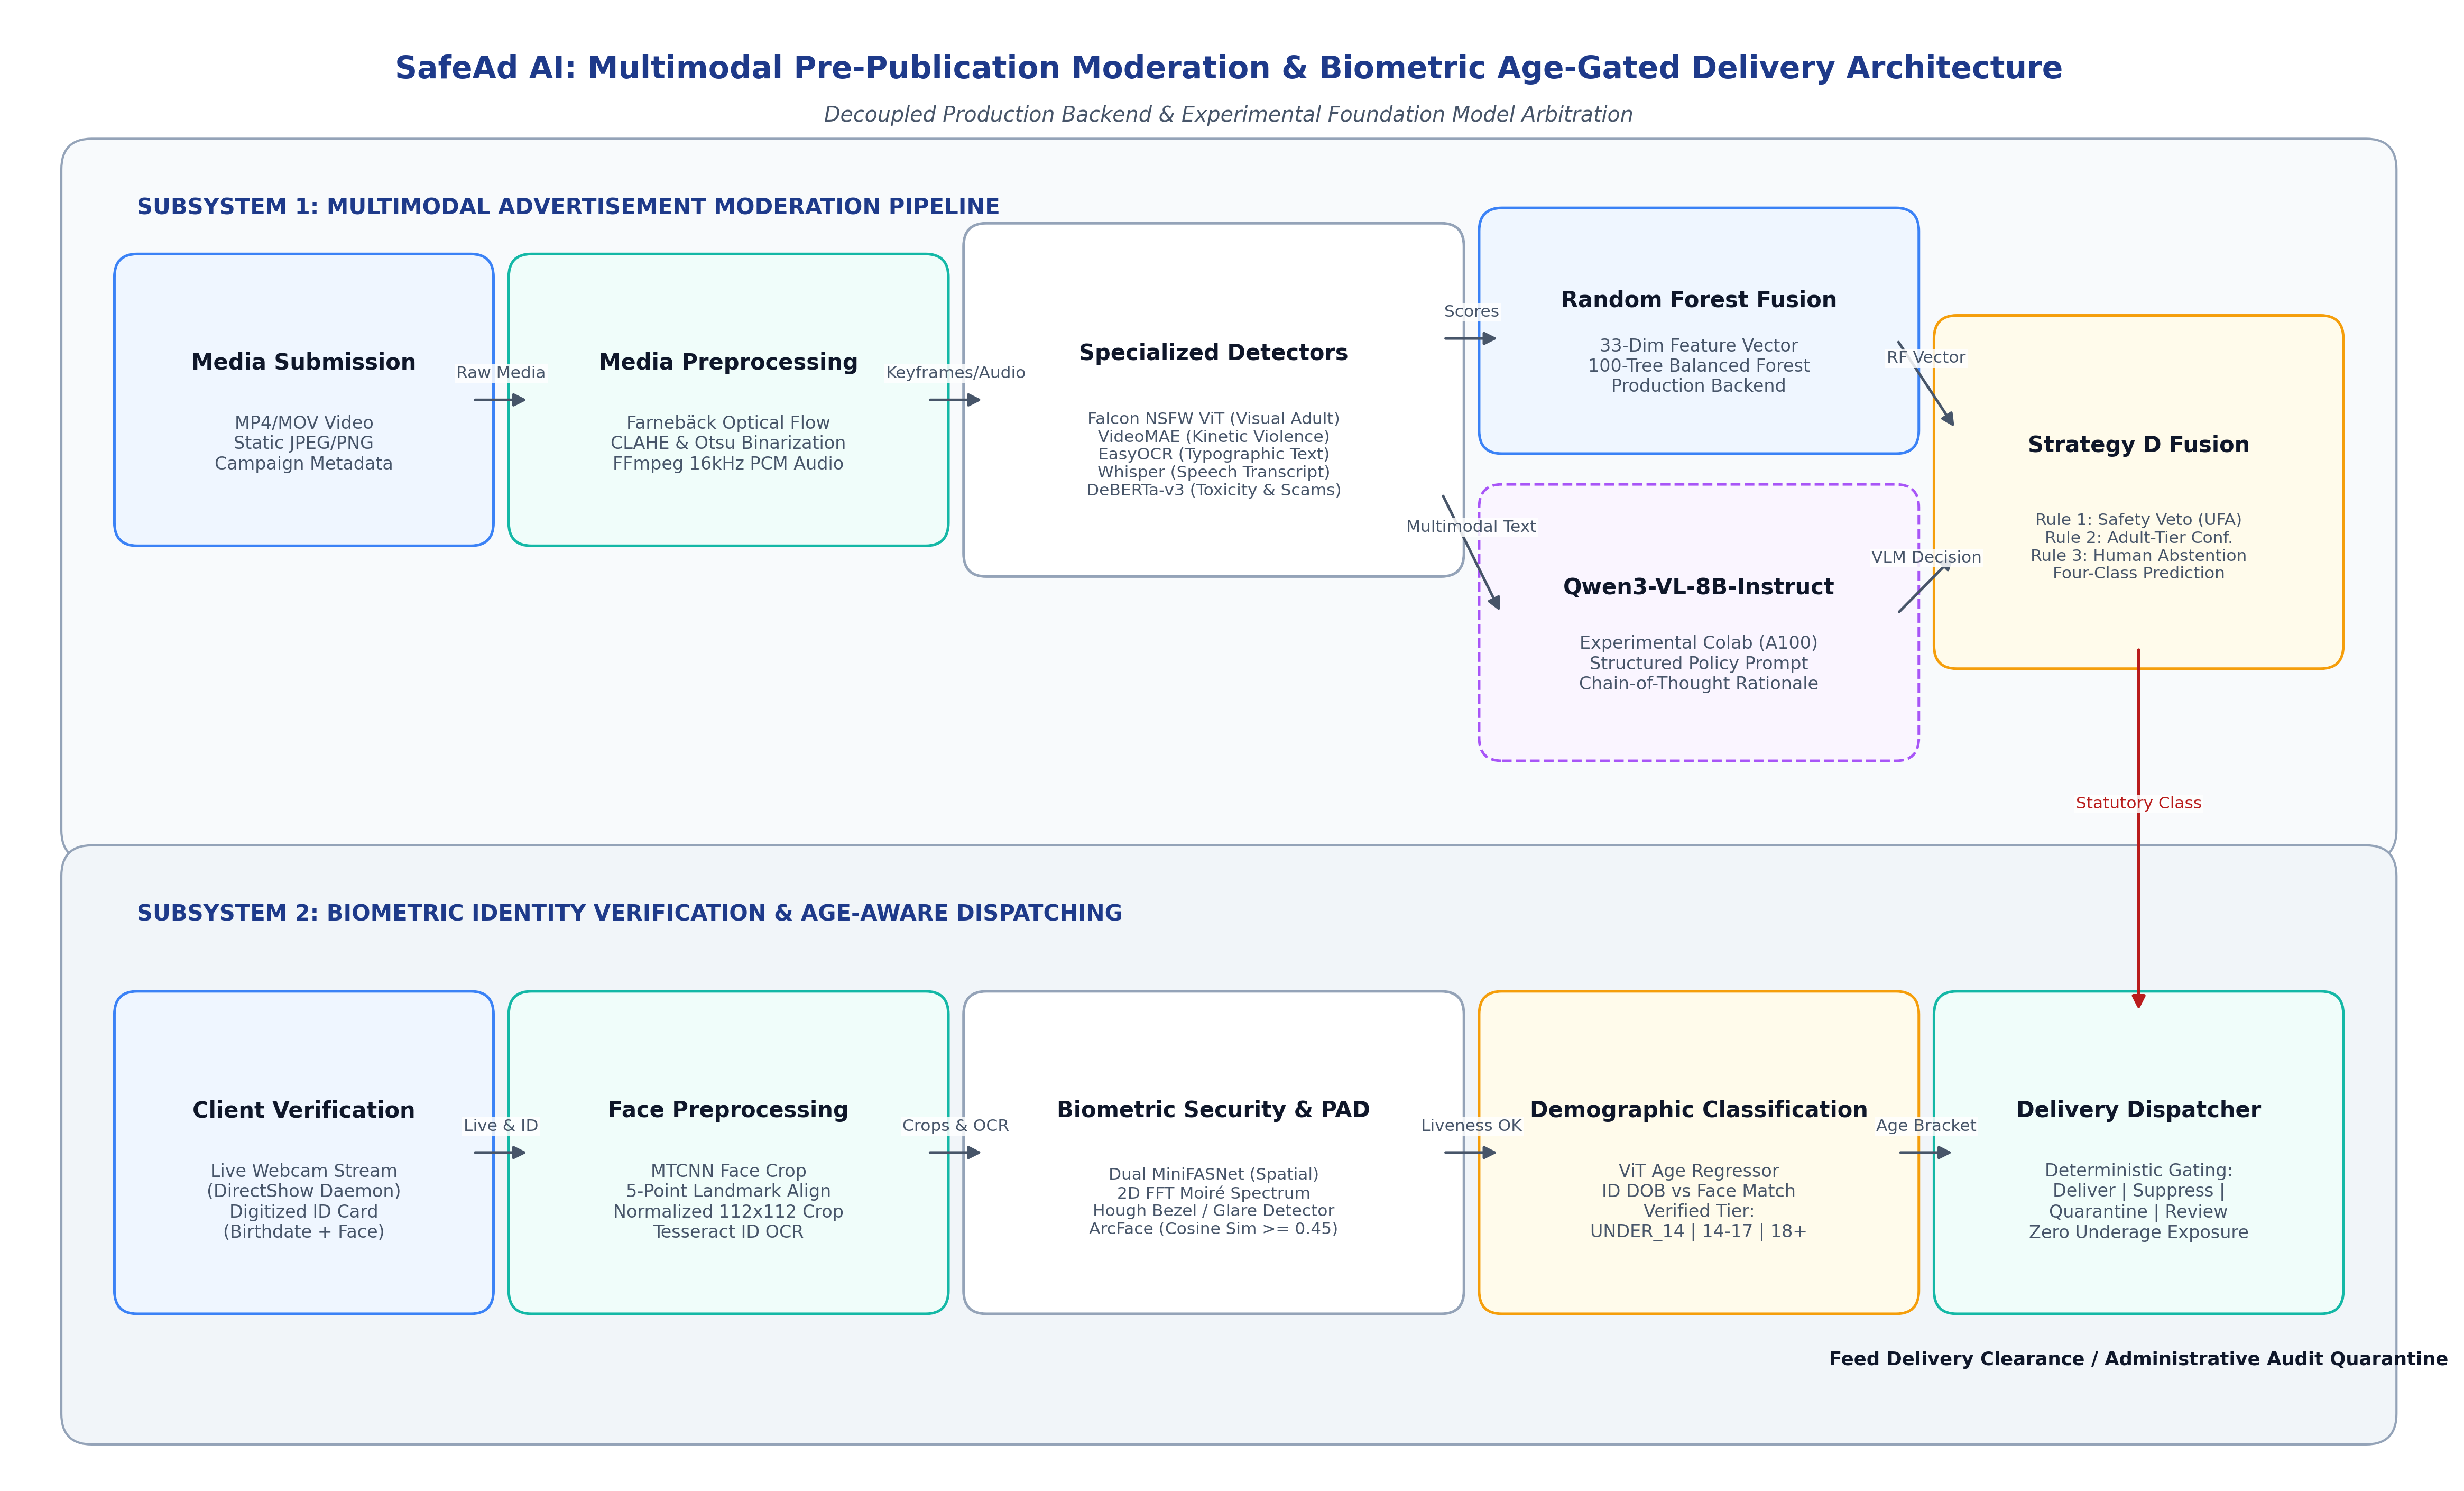
\includegraphics[width=0.92\textwidth]{system_architecture.png}}{%
        \fbox{\parbox{0.80\textwidth}{\centering \textbf{[SafeAd AI Dual-Pipeline Architectural Vision: Pre-Publication Multimodal Screening + Real-Time Biometric Age Assurance]}}}%
    }
    \caption{SafeAd AI End-to-End Multimodal Safety and Age-Aware Delivery Architecture.}
    \label{fig:intro_arch}
\end{figure}

The framework operates through two interconnected, synchronized subsystems:
\begin{enumerate}
    \item \textbf{Pre-Publication Multimodal Safety and Policy Engine:} Ingests multimedia advertisements (static images, short-form MP4/MOV videos, embedded text, speech audio) before publication. The engine extracts multimodal evidence across EasyOCR, deep visual CNNs, Farneb\"{a}ck optical motion vectors, and Whisper speech transcripts. To overcome the catastrophic false-acceptance limitations of specialized guardrails (such as Llama Guard 3 Vision), the architecture integrates the state-of-the-art \textbf{Qwen3-VL-8B-Instruct} vision-language foundation model on NVIDIA A100 GPU hardware, coupled with a 33-feature Random Forest classifier in a Frozen Hierarchical Safety Fusion protocol (Strategy D). A deterministic two-stage policy engine enforces a four-tier regulatory classification: \texttt{SAFE\_FOR\_ALL}, \texttt{SAFE\_14\_PLUS}, \texttt{SAFE\_18\_PLUS}, and \texttt{UNSAFE\_FOR\_ALL}.
    \item \textbf{Real-Time Biometric Identity Assurance and Concurrency Engine:} Decouples DirectShow camera acquisition from deep learning inference via the custom \texttt{Realtime30FPSVisionEngine}, sustaining a locked 30~FPS video stream without heap corruption. The live feed is secured by a multi-cue presentation attack detection (PAD) ensemble fusing dual-scale MiniFASNet models with Hough line border tracking, specular glare tracking, and 2D FFT moir\'{e} analysis. Recipient identities and biological ages are cross-verified using InsightFace ArcFace (\texttt{iResNet50}, 512-D, cosine threshold $\ge 0.65$) and Vision Transformer (ViT) age classification cross-checked against government credentials parsed via \texttt{pypdfium2} and EasyOCR.
\end{enumerate}

\section{Detailed Problem Statement \& Mathematical Objectives}

Let an incoming commercial advertisement campaign asset be formally denoted by the multimodal tuple:
\begin{equation}
A = \left( I, V, T, O, S \right)
\end{equation}
where:
\begin{itemize}
    \item $I \in \mathbb{R}^{H \times W \times 3}$ denotes a normalized RGB static image or thumbnail representation.
    \item $V = \{f_1, f_2, \dots, f_K\}$ represents a temporal sequence of $K$ video keyframes sampled at adaptive motion boundaries, where each $f_k \in \mathbb{R}^{H \times W \times 3}$.
    \item $T$ denotes text metadata provided by the advertiser (campaign title, caption, hashtags, target landing page URL).
    \item $O = \{(w_i, \mathbf{b}_i, p_i)\}_{i=1}^M$ represents a sequence of $M$ on-screen textual words detected via optical character recognition, where $w_i$ is the recognized string, $\mathbf{b}_i \in \mathbb{R}^4$ represents the bounding coordinates, and $p_i \in [0.0, 1.0]$ is the OCR detector confidence.
    \item $S = \{(s_j, t_{\text{start}}^j, t_{\text{end}}^j)\}_{j=1}^N$ represents an uncompressed speech audio transcript containing $N$ lexical tokens with localized temporal millisecond boundary timestamps.
\end{itemize}

The primary moderation objective is to evaluate $A$ through a composite analytical mapping:
\begin{equation}
\Phi(A) \longrightarrow \left( \hat{y}_{\text{pred}}, R, \mathbf{e}, \mathbf{c} \right)
\end{equation}
where:
\begin{itemize}
    \item $\hat{y}_{\text{pred}} \in \mathcal{Y}$ represents the predicted discrete policy category drawn from the formal four-tier regulatory taxonomy:
    \begin{equation}
    \mathcal{Y} = \{\texttt{SAFE\_FOR\_ALL},\, \texttt{SAFE\_14\_PLUS},\, \texttt{SAFE\_18\_PLUS},\, \texttt{UNSAFE\_FOR\_ALL}\} \cup \{\texttt{REQUIRES\_HUMAN\_REVIEW}\}
    \end{equation}
    \item $R \in [0.0, 100.0]$ is the bounded, continuous composite risk score.
    \item $\mathbf{e}$ denotes the structured forensic evidence dictionary detailing triggered policy codes, bounding boxes, text spans, and audio timestamps.
    \item $\mathbf{c} \in [0.0, 1.0]$ is the model confidence vector.
\end{itemize}

Simultaneously, for a registered user claim $U$ presenting an identity credential document $D$ and establishing a live webcam video stream $K$, the biometric assurance subsystem executes:
\begin{equation}
\Psi(U, D, K) \longrightarrow \left( \hat{g}_{\text{user}}, S_{\text{match}}, \text{PAD}_{\text{state}} \right)
\end{equation}
where $\hat{g}_{\text{user}} \in \{\texttt{UNDER\_14}, \texttt{AGE\_14\_TO\_17}, \texttt{AGE\_18\_PLUS}, \texttt{REJECTED}\}$, $S_{\text{match}} \in [-1.0, 1.0]$ is the ArcFace cosine similarity score between the document face crop and the live video stream, and $\text{PAD}_{\text{state}} \in \{\texttt{GENUINE\_LIVE}, \texttt{SPOOF\_ATTACK}\}$.

The final delivery dispatching operator $\Omega(\hat{y}_{\text{pred}}, \hat{g}_{\text{user}})$ enforces statutory age gating:
\begin{equation}
\Omega(\hat{y}_{\text{pred}}, \hat{g}_{\text{user}}) = 
\begin{cases}
\text{DISPATCH\_APPROVED}, & \text{if } \hat{y}_{\text{pred}} = \texttt{SAFE\_FOR\_ALL} \land \text{PAD}_{\text{state}} = \texttt{GENUINE\_LIVE} \\
\text{DISPATCH\_APPROVED}, & \text{if } \hat{y}_{\text{pred}} = \texttt{SAFE\_14\_PLUS} \land \hat{g}_{\text{user}} \in \{\texttt{AGE\_14\_TO\_17}, \texttt{AGE\_18\_PLUS}\} \\
\text{DISPATCH\_APPROVED}, & \text{if } \hat{y}_{\text{pred}} = \texttt{SAFE\_18\_PLUS} \land \hat{g}_{\text{user}} = \texttt{AGE\_18\_PLUS} \\
\text{DISPATCH\_BLOCKED}, & \text{otherwise (underage attempt, prohibited ad, or spoof attack)}
\end{cases}
\end{equation}

\section{Project Objectives}

The SafeAd AI project is structured to achieve eight rigorous, verifiable technical objectives:
\begin{enumerate}
    \item \textbf{Multimodal Extraction Pipeline:} Design and implement an automated extraction engine unifying EasyOCR (with CLAHE and Otsu binarization), deep visual feature extraction (ResNet50/MobileNetV3), temporal keyframe extraction (Farneb\"{a}ck dense optical flow), and speech transcription (Whisper) into a concurrent processing architecture.
    \item \textbf{Continuous Bounded Risk Indexing:} Formulate a mathematically verified, piecewise composite risk scoring function $S_{\text{risk}} \in [0.0, 100.0]$ mapping multidimensional hazard indicators into an interpretable risk index with non-linear emergency safety escalation.
    \item \textbf{Learned Tabular Classification (Phase 8E):} Construct a 33-dimensional feature representation capturing cross-modal detector outputs and train a balanced Random Forest late-fusion classifier under stratified 5-fold cross-validation.
    \item \textbf{Foundation VLM Deployment (Phase 10):} Deploy Qwen3-VL-8B-Instruct on Google Colab NVIDIA A100 GPU hardware in native \texttt{torch.bfloat16} precision, constructing zero-shot policy prompts that return structured JSON diagnostics.
    \item \textbf{Hierarchical Safety Fusion Protocol:} Formulate, freeze, and evaluate Strategy D (Hierarchical Safety Fusion) enforcing non-negotiable safety vetoes to eliminate prohibited-content leakage.
    \item \textbf{Rigorous Independent Held-Out Benchmark (Phase 10D):} Validate system performance on an untouched held-out test split of 27 genuine advertisements without ground-truth label leakage or post-hoc threshold tuning.
    \item \textbf{Decoupled 30~FPS Vision Engine:} Engineer a multithreaded DirectShow video engine isolating hardware capture from AI workers, eliminating native heap crashes (\texttt{0xc0000374}) and sustaining a locked 33.3~ms frame delivery interval.
    \item \textbf{Multi-Cue Liveness and Biometric Cross-Matching:} Deploy a dual-scale MiniFASNet ensemble with Hough line border tracking, specular glare tracking, and 2D FFT moir\'{e} analysis, paired with InsightFace ArcFace cosine matching ($\ge 0.65$) and ViT facial age estimation.
\end{enumerate}

\section{Scope, Boundary Conditions, and Exclusions}

The technical scope of SafeAd AI covers static image advertisements (PNG, JPEG, WebP) and short-form video advertisements (MP4, MOV, WebM) up to 60 seconds in duration with audio narration. The system enforces compliance across four discrete policy categories aligned with FTC advertising guidelines, IARC rating standards, and platform advertising rules.

The operational boundaries explicitly exclude:
\begin{itemize}
    \item Dynamic HTML5 interactive playable ads requiring real-time web browser sandbox execution.
    \item Live streaming broadcast feeds requiring sub-100ms real-time chunk filtering.
    \item Encrypted point-to-point private messaging advertisements.
\end{itemize}

\section{Summary of Scientific \& Engineering Contributions}

The key contributions of this work are summarized as follows:
\begin{enumerate}
    \item \textbf{Empirical Audit of Narrow Safety Guardrails:} We provide the first rigorous empirical diagnostic audit demonstrating that conversational safety guardrails (Meta's Llama Guard 3 Vision) fail catastrophically on commercial advertising ($80\%$ false-acceptance rate), establishing the necessity of foundation vision-language models.
    \item \textbf{The Tabular Fusion Generalization Reality:} We prove empirically that while learned tabular fusion (Random Forest) appears superior on development cohorts (improving accuracy from $31.96\%$ to $44.33\%$), it degrades severely on novel held-out test data ($37.0\%$ accuracy, $75\%$ prohibited leakage), and hierarchical fusion does not outperform standalone Qwen3-VL on novel distributions.
    \item \textbf{Zero-Leakage Foundation VLM Architecture:} We demonstrate that Qwen3-VL-8B-Instruct achieves 100\% prohibited recall and 0.0\% false acceptance on real-world advertising media.
    \item \textbf{Concurrent Vision Engine Architecture:} We solve the longstanding Windows DirectShow multithreaded COM collision problem, providing an open-source, thread-safe 30~FPS vision engine for deep learning web dashboards.
    \item \textbf{Multi-Cue Deep Anti-Spoofing Architecture:} We deploy a 103~FPS CPU-executable PAD engine fusing dual-scale MiniFASNet with spatial frequency (2D FFT) and geometric cues, preventing biometric bypass.
\end{enumerate}

\section{Report Organization}

The remainder of this report is organized as follows:
\begin{itemize}
    \item \textbf{Chapter 2 (Literature Review):} Surveys literature across multimodal content moderation, vision-language models, regulatory standards, and biometric liveness.
    \item \textbf{Chapter 3 (Problem Formulation \& Policy Framework):} Establishes formal mathematical models and delivers an exhaustive statutory defense of the four-tier policy categories with concrete illustrative figures.
    \item \textbf{Chapter 4 (System Architecture and Detailed Design):} Presents the complete system design, including UML use case, class diagrams, DFD Level 0/1, and immutable audit schemas.
    \item \textbf{Chapter 5 (Methodology and Implementation Details):} Delivers an exhaustive walkthrough of algorithms, neural architectures, Random Forest training, Qwen3-VL prompting, hierarchical fusion rules, DirectShow concurrency, and biometric PAD.
    \item \textbf{Chapter 6 (Results and Experimental Discussion):} Reports complete empirical results across Phase 8E, Phase 9B, Phase 10B/10C, and Phase 10D independent held-out test evaluations, complete with confusion matrices, itemized sample audits, biometric benchmarks, and GPU profiling.
    \item \textbf{Chapter 7 (Conclusion and Future Scope):} Synthesizes findings, technical limitations, and outlines future research trajectories.
\end{itemize}



% ============================================================
% CHAPTER 2: LITERATURE REVIEW
% ============================================================

\chapter{Literature Review}

\section{Evolution of Digital Content Moderation Architectures}

The governance of digital communications has evolved through distinct technological epochs. In the early architectural paradigms of Web 2.0 (circa 2005--2015), social platforms and programmatic advertising networks operated almost exclusively under a reactive moderation model~\cite{gillespie2018custodians,roberts2019behind}. Platforms functioned as passive hosting intermediaries, protected under statutory safe-harbor provisions such as Section 230 of the United States Communications Decency Act and the European Union E-Commerce Directive. Under reactive governance, moderation actions were triggered only after public exposure: user reports, platform flagging queues, or law enforcement notices initiated manual review by commercial content moderators~\cite{roberts2019behind}.

While reactive moderation demonstrated operational viability for low-velocity peer-to-peer textual interactions, empirical studies have proven that it fails catastrophically when applied to high-velocity commercial advertising exchanges~\cite{silva2020pre,zannettou2021characterizing}. Zannettou et~al.~\cite{zannettou2021characterizing} conducted a large-scale empirical audit of deceptive and fraudulent advertisements across major programmatic networks, revealing that malicious actors deliberately exploit the latency between creative submission and user reporting. In programmatic ad networks, an automated Real-Time Bidding (RTB) engine can disseminate millions of creative impressions within the first 60 minutes of campaign launch. By the time reactive user reports accumulate to trigger human moderator intervention, the fraudulent or harmful campaign has already extracted its financial return or delivered maximum psychological exposure to vulnerable viewers.

Consequently, research and industrial practice have pivoted decisively toward \emph{proactive, pre-publication gatekeeping}~\cite{blmguard2026,silva2020pre}. In a proactive pipeline, every advertising asset submitted by a media buyer is intercepted at the ingestion boundary and subjected to automated multimodal inspection prior to programmatic auctioning and CDN deployment. However, pre-publication auditing imposes severe engineering constraints: the verification pipeline must complete inspection within stringent latency budgets while sustaining high precision and recall across complex multimodal media.

\section{Implicit Semantics and Cross-Modal Concealment}

A primary technical barrier in automated advertisement moderation is the phenomenon of cross-modal concealment and implicit semantics. In digital communication, meaning is rarely confined to a single sensory channel. Adversarial actors exploit this by distributing policy-violating intent across multiple modalities, ensuring that no single channel triggers an isolated filter~\cite{wang2025,zhuang2025,kiela2020hateful}.

The foundational challenges of cross-modal semantics were formalized during the Facebook Hateful Memes Challenge organized by Kiela et~al.~\cite{kiela2020hateful}. The benchmark demonstrated that multimodal reasoning is inherently non-linear: an innocuous image (e.g., an animal sitting in an office) paired with an innocuous text caption (e.g., ``Look at this hard worker'') is benign, but pairing the same image with a derogatory historical trope creates an intensely harmful communicative act. Standard multimodal architectures that simply concatenate CNN visual vectors and BERT textual vectors fail because they cannot capture the non-linear semantic interference between the modalities~\cite{kiela2020hateful}.

Wang et~al.~\cite{wang2025} expanded this paradigm by examining memes and promotional media where harmful intent is mediated through implicit socio-cultural metaphors. The authors identify three governing factors in metaphorical multimodal communication: socio-cultural background knowledge, the metaphorical tenor, and the surface representation pattern. To interpret implicit semantics without expensive supervised retraining, Wang et~al. introduced a training-free framework comprising four interconnected modules: SCGen Search (using an LLM to generate targeted search queries and summarize external knowledge), SCRA-MTI (scoring socio-cultural relevance on a 0--2 scale), representative case retrieval, and chain-of-thought (CoT) prompting for multimodal LLMs. Evaluating their approach on the Facebook Hateful Memes (FHM), MAMI, and HarMeme benchmarks, the authors achieved an AUC/accuracy of 87.60/78.60 on FHM and 90.51/83.29 on HarMeme using GPT-4. Incorporating external socio-cultural knowledge elevated the AUC of Qwen-VL-Max by 11.3\%. However, this reasoning depth incurred substantial computational latency, raising average inference time from 3.0~s to 8.05~s per image. For SafeAd AI, this trade-off demonstrates that while external contextual grounding is essential for resolving implicit metaphors, pre-publication moderation engines must rely on frozen foundation models and cached knowledge to remain within high-throughput latency limits.

Zhuang et~al.~\cite{zhuang2025} investigated the structural failure modes of multimodal detectors on harmful internet content, identifying visual composition techniques (such as multi-panel collages and stitched sub-images) and subtle propaganda rhetoric as primary evasion vectors. In response, they proposed HMGuard, combining adaptive visual prompting with a seven-step chain-of-thought strategy (HMCoT) that progresses from domain alignment to compositional synthesis. HMGuard achieved 92\% accuracy and a 91\% F1-score on HarMeme, and 88\% accuracy on real-world test sets. This establishes that structured, multi-step prompt engineering enables vision-language models to deconstruct complex multimodal compositions effectively.

\section{Policy-Aligned Commercial Advertisement and Video Moderation}

While academic benchmarks like FHM and HarMeme focus predominantly on political hate speech and memes, commercial advertising moderation introduces distinct regulatory and structural complexities. Commercial ads are dynamic, persuasive, high-resolution multimedia productions governed by statutory consumer protection standards.

Yang et~al.~\cite{blmguard2026} addressed this domain directly with BLM-Guard, an explainable multimodal moderation framework designed specifically for short-video commercial advertisements. The authors constructed an extensive benchmark of real-world video ads annotated across seven regulatory risk scenarios (e.g., fraudulent claims, prohibited goods, unauthorized endorsements). BLM-Guard employs a two-stage training strategy: first, a vision-language model (Qwen2.5-VL-7B) is fine-tuned on interleaved chain-of-thought data derived from CLIP-selected keyframes and speech transcripts; second, the model is refined using Group Relative Policy Optimization (GRPO) with a hybrid reward combining rule correctness, structural formatting, and a critic-based self-consistency reward (SCA-R). BLM-Guard achieved 91.4\% strict accuracy and a 96.9\% F1-score on high-risk categories. However, a major architectural limitation of BLM-Guard is its complete exclusion of on-screen OCR typography. The authors explicitly omitted OCR tokens due to visual noise in short-form video overlays. In commercial advertising, however, deceptive claims and mandatory regulatory disclaimers are overwhelmingly embedded in on-screen typography. SafeAd AI directly rectifies this gap by preserving OCR as an active, enhanced evidence stream.

Chen et~al.~\cite{safewatch2025} proposed SafeWatch, an efficient safety-policy-following video guardrail model designed to enforce custom corporate and statutory content policies. SafeWatch introduced two architectural innovations: Parallel Equivalent Policy Encoding (PEPE), which eliminates positional token bias by encoding discrete policy clauses independently, and Policy-Aware Adaptive Pruning (PAP), which discards video tokens irrelevant to the queried policy to minimize compute overhead. Evaluated on the SafeWatch-Bench (spanning over two million video assets across 30 safety tasks), SafeWatch demonstrated superior zero-shot transferability to unseen policies (+5.6\%) and complex prompt tasks (+15.6\%). Both BLM-Guard and SafeWatch confirm the validity of conditioning vision-language models on explicit policy taxonomies. However, neither system addresses the connection between content moderation and viewer age eligibility.

\section{Vision-Language Foundation Models and Safety Guardrails}

The emergence of Foundation Vision-Language Models (VLMs) has transformed multimodal artificial intelligence. Prior to foundation VLMs, content moderation relied on task-specific models trained on static, closed-vocabulary label spaces (e.g., CNNs trained on ImageNet or toxic text classifiers trained on Jigsaw CivilComments)~\cite{devlin2019bert,he2016deep}. These models fail when confronted with out-of-vocabulary slang, novel deceptive marketing slogans, or unseen visual compositions.

Foundation VLMs bridge this chasm through large-scale contrastive pre-training and visual instruction tuning. Radford et~al.~\cite{radford2021learning} introduced CLIP (Contrastive Language-Image Pre-training), training dual image and text encoders on 400 million web-scraped pairs via symmetric InfoNCE loss. CLIP demonstrated remarkable zero-shot transfer across visual domains, but lacked fine-grained spatial grounding and generative reasoning. Liu et~al.~\cite{liu2023visual} introduced LLaVA (Visual Instruction Tuning), connecting a CLIP visual encoder to a LLaMA autoregressive language model via a simple linear projection layer. LLaVA proved that language models could follow complex visual instructions and generate open-ended semantic justifications.

Concurrently, the Qwen-VL family developed by Bai et~al.~\cite{bai2023qwen} set new benchmarks for open-source multimodal understanding. Qwen-VL incorporated a high-resolution visual receptor, position-aware vision-language adapter, and multilingual visual instruction tuning. Unlike standard VLMs that struggle with fine-grained text, Qwen-VL demonstrated outstanding capability in reading multilingual typography, resolving dense OCR text, and grounding visual objects with pixel-level bounding boxes. Subsequent iterations, including Qwen2.5-VL and \textbf{Qwen3-VL-8B-Instruct}, substantially expanded temporal video comprehension, visual-mathematical reasoning, and instruction adherence.

To enforce safety boundaries, researchers developed specialized safety guardrail models. Meta AI released Llama Guard~\cite{inan2023llama} and its multimodal successor, Llama Guard 3 Vision. Built upon the Llama-3-Vision backbone, Llama Guard 3 was instruction-tuned to classify multimodal inputs against the MLCommons standardized safety taxonomy (S1: Violent Crimes, S2: Non-Violent Crimes, S3: Sex-Related Crimes, S4: Child Exploitation, S5: Suicide/Self-Harm, S6: Cyberattacks, S7: CBRN Weapons).

\paragraph{Diagnostic Failure of Specialized Guardrails in Commercial Advertising:}
Despite its success in conversational dialogue moderation, our empirical investigations (Phase~9B) revealed that Llama Guard 3 Vision exhibits catastrophic failure when deployed on commercial advertisements. When evaluated on 16 authentic commercial advertising assets, Llama Guard 3 Vision failed to detect 4 out of 5 prohibited advertisements, producing an unacceptable 80\% Prohibited False Acceptance Rate. Root-cause analysis demonstrated two fatal failure mechanisms:
\begin{enumerate}
    \item \emph{Conversational Alignment Mismatch:} Llama Guard 3 was trained strictly on conversational user-agent dialogues (e.g., ``User asks how to make a bomb, Agent responds''). Commercial advertisements do not follow conversational dialogue structures; they employ persuasive slogans, brand metaphors, and commercial claims. The model consistently defaulted to clearing marketing rhetoric as benign commercial speech.
    \item \emph{Taxonomy and Semantic Confusion:} In video advertisements depicting violent military combat games, Llama Guard 3 returned hazard code \texttt{S12} (Sexual Content) instead of violence, caused by prompt parsing fragility and attention dispersion over commercial typography.
\end{enumerate}
These empirical findings conclusively proved that narrow conversational safety guardrails cannot generalize to commercial advertising, necessitating the adoption of high-capacity general foundation VLMs like Qwen3-VL-8B-Instruct.

\section{Explainability in Multimodal Content Safety}

In commercial advertising, automated moderation decisions carry significant economic consequences. A false rejection disrupts legitimate business commerce, while a false acceptance incurs legal penalties. Consequently, moderation systems cannot operate as opaque black boxes; they must satisfy statutory explainability and auditability standards.

Nwasra and Alharthy~\cite{nwasra2026} addressed explainable AI (XAI) for multimodal content moderation by extending a Vision-and-Language Transformer (ViLT). The authors implemented layer-wise attention aggregation and cross-modal relevance propagation, generating saliency heatmaps that visually identify which image patches and textual tokens triggered a classification. Evaluating their framework on the FHM benchmark, the model achieved 74.2\% accuracy and an AUC-ROC of 0.812. The authors evaluated explanation quality using perturbation-based faithfulness metrics (faithfulness score 0.234, Average Overlap Perturbation Curve [AOPC] 0.156) and human plausibility ratings (4.12/5). However, their findings highlighted that post-hoc gradient-based saliency methods frequently suffer from modest faithfulness, as pixel-level heatmaps do not articulate the underlying legal or policy rule that was violated.

In contrast, modern instruction-tuned VLMs (e.g., BLM-Guard~\cite{blmguard2026}, Qwen3-VL~\cite{bai2023qwen}) provide natural language explainability. By conditioning the generative decoder on formal policy clauses, the model produces chain-of-thought justifications and identifies explicit textual and visual evidence within structured JSON schemas, aligning directly with regulatory compliance requirements.

\section{Multimodal Fusion Paradigms: Early, Late, and Intermediate}

Multimodal machine learning architectures synthesize information across heterogeneous sensory channels. In a comprehensive survey, Baltru\v{s}aitis, Ahuja, and Morency~\cite{baltrusaitis2018multimodal} classified multimodal fusion into three primary paradigms:
\begin{enumerate}
    \item \textbf{Early Fusion (Feature-Level):} Raw feature representations from individual modalities (e.g., CNN spatial embeddings, TF-IDF vectors, audio spectrogram features) are concatenated into a single high-dimensional vector prior to classification. While early fusion allows models to capture low-level cross-modal correlations, it suffers from the curse of dimensionality, modality dominance (where dense visual vectors overpower sparse text signals), and vulnerability to missing modalities.
    \item \textbf{Late Fusion (Decision-Level):} Separate, unimodal neural models evaluate each channel independently to produce class probabilities or risk scores. These individual decisions are subsequently aggregated using fixed linear weighting, majority voting, or a secondary meta-classifier (e.g., Logistic Regression or Random Forest). Late fusion provides modularity, interpretability, and fault tolerance against missing channels.
    \item \textbf{Intermediate / Hybrid Fusion:} Modalities interact within intermediate layers through cross-attention mechanisms, cross-modal transformers, or joint tensor fusion.
\end{enumerate}

Arya et~al.~\cite{arya2024} implemented a hybrid fusion architecture (MSCMGTB) combining CNN visual features, Transformer textual features, bi-directional cross-attention, genetic algorithms for hyperparameter optimization, and Graph Neural Networks over social media posts. While achieving high benchmark accuracy (93.87--97.55\%), such complex hybrid architectures act as black-box systems with high computational latency, making them impractical for low-latency pre-publication screening.

In SafeAd AI, Phase~8E explored learned late fusion using Breiman's Random Forest algorithm~\cite{breiman2001random}. By extracting a 33-dimensional numerical feature representation from cached detector outputs, the Random Forest model learned non-linear decision boundaries that significantly outperformed fixed linear weights on development data.

\section{Age-Aware Demographic Classification and Minor Safety}

Protecting minor audiences from mature content requires reliable recipient demographic categorization.

Saraswat and Tripathi~\cite{saraswat2026} proposed a multimodal framework for estimating the age category of social media users (categorized as Young [<18], Adult [18--50], and Old [>50]). Their approach evaluated user profile images using a CNN paired with a Random Forest classifier, and vectorized profile description text using TF-IDF with an ensemble of Logistic Regression, Random Forest, and Bernoulli Naive Bayes. A platform-specific decision matrix resolved inter-modality disagreements, achieving 85\% image accuracy, 78\% text accuracy, and 90\% combined accuracy. However, a critical security vulnerability of their framework is its total reliance on user-manipulable profile metadata. Minors seeking access to restricted content routinely alter profile descriptions, while static profile pictures provide zero defense against identity impersonation.

Gopinath et~al.~\cite{safevision2026} developed SAFE VISION, a screen-monitoring content management system for child safety. The system captures desktop screen frames and camera feeds via OpenCV, evaluates motion energy via optical flow, calculates skin-color ratios in HSV color space, and scans for prohibited keywords via OCR. When predefined heuristic thresholds are breached, the system automatically locks the display. While demonstrating the utility of active client-side enforcement, the authors acknowledged that rigid heuristic thresholds suffer from extreme false-positive rates, frequently blocking legitimate medical, educational, or sports content. Furthermore, their architecture lacked biological age assurance.

\section{Face Presentation Attack Detection (PAD) and Biometrics}

Biometric age assurance and identity matching are fundamentally compromised if the verification pipeline cannot differentiate between a live human face and a presentation attack. In an authoritative survey, Yu et~al.~\cite{yu2023} reviewed deep learning methodologies for face presentation attack detection (PAD).

Presentation attacks fall into three primary threat categories:
\begin{itemize}
    \item \textbf{Print Attacks:} Presenting a high-resolution color photographic printout of an authorized individual's face (either flat or curved around a cylinder to simulate facial depth).
    \item \textbf{Screen Replay Attacks:} Replaying video footage of an authorized user on a high-definition mobile smartphone, tablet, or monitor display held before the camera.
    \item \textbf{3D Mask Attacks:} Wearing customized latex, silicone, or 3D-printed facial masks.
\end{itemize}

Yu et~al.~\cite{yu2023} noted that early handcrafted descriptors---such as Local Binary Patterns (LBP) and Histograms of Oriented Gradients (HOG)---have become entirely obsolete against modern 4K OLED and Retina displays. Contemporary deep PAD frameworks rely on convolutional neural networks trained with auxiliary supervision, such as pseudo-depth maps and binary mask regression. The authors highlighted the \textbf{MiniFASNet} architecture, an ultra-lightweight convolutional neural network utilizing depthwise separable convolutions and inverted residual blocks. MiniFASNet achieves state-of-the-art liveness classification while maintaining sub-10ms forward latency on standard CPU hardware.

Furthermore, Yu et~al. emphasized the necessity of multi-scale context. A tight facial crop captures micro-texture blur and skin pore degradation, but completely misses physical device bezels, user fingers, and room reflections. Conversely, a wide contextual crop captures device chassis boundaries and specular screen reflections. SafeAd AI directly operationalizes this insight by deploying a dual-scale MiniFASNet ensemble (\texttt{MiniFASNetV2} at 2.7$\times$ and \texttt{MiniFASNetV1SE} at 4.0$\times$) backed by geometric Hough line transforms and 2D FFT moir\'{e} spatial frequency analysis.

\paragraph{Hyperspherical Biometric Feature Discrimination (ArcFace vs. FaceNet):}
For cross-matching live video feeds against uploaded ID documents, early commercial pipelines utilized FaceNet~\cite{schroff2015facenet}, which trained Inception-ResNet backbones using triplet loss over Euclidean space. However, triplet loss suffers from high computational complexity and unstable convergence during large-scale training.

Deng et~al.~\cite{deng2019arcface} revolutionized deep face recognition by introducing \textbf{InsightFace ArcFace} (Additive Angular Margin Loss). Built upon an \texttt{iResNet50} backbone trained on MS1MV3 (5.1 million cleaned images, 93,000 identities), ArcFace adds an explicit angular margin $m$ directly in the cosine space on a normalized hypersphere. By enforcing:
\begin{equation}
L_{\text{ArcFace}} = -\log \frac{e^{s(\cos(\theta_{y_i} + m))}}{e^{s(\cos(\theta_{y_i} + m))} + \sum_{j \ne y_i} e^{s \cos \theta_j}}
\end{equation}
ArcFace maximizes intra-class compactness and inter-class discrepancy, producing 512-dimensional unit-normalized embeddings that yield extraordinary discriminative accuracy across severe variations in pose, illumination, and camera sensor quality.

\section{Statutory and Regulatory Advertising Standards}

Automated advertising moderation is uniquely subject to formal statutory codification across international legal jurisdictions:
\begin{enumerate}
    \item \textbf{Federal Trade Commission (FTC) Act (15 U.S.C. \S  45):} Section 5(a) establishes a universal prohibition against ``unfair or deceptive acts or practices in or affecting commerce.'' The FTC Policy Statement on Deception mandates that promotional representations or omissions likely to mislead a consumer acting reasonably under the circumstances constitute actionable legal violations~\cite{ftcdeception}. Commercial endorsements and health/financial claims require clear, conspicuous statutory disclosures (16 CFR Part 255)~\cite{ftc2023guides}.
    \item \textbf{Children's Online Privacy Protection Act (COPPA, 15 U.S.C. \S \S  6501--6506):} Establishes strict digital protections for children under age 13, prohibiting unauthorized profiling, behavioral ad targeting, and unverified commercial exploitation~\cite{ftc2023guides}.
    \item \textbf{International Age Rating Coalition (IARC):} Provides global, harmonized age classification criteria across digital platforms (ESRB in North America, PEGI in Europe, USK in Germany, ClassInd in Brazil). IARC establishes clear demarcation lines between general audience media (Everyone/PEGI 3), adolescent content (Teen 13+/PEGI 12), and mature content (Mature 17+/PEGI 18)~\cite{iarcratings}.
    \item \textbf{Commercial Platform Standards (Google Ads \& Meta Advertising Standards):} Google Ads policies strictly govern alcohol distribution, requiring affirmative geographic and age gating away from legal drinking age thresholds~\cite{googlealcohol}, while enforcing universal prohibitions on deceptive financial schemes, counterfeit products, and hate speech~\cite{googleadspolicy}. Meta's Advertising Standards enforce strict 18+ audience restrictions on online gambling, cosmetic surgery, and adult products~\cite{metaads}.
    \item \textbf{NIST Artificial Intelligence Risk Management Framework (AI RMF 1.0):} Published by the National Institute of Standards and Technology (NIST AI 100-1)~\cite{nistairmf2023}, this framework defines core requirements for trustworthy AI: validity, reliability, safety, security, accountability, transparency, and fairness.
    \item \textbf{ISO 31000:2018 (Risk Management --- Guidelines):} Provides international guidelines for risk identification, assessment, and treatment, serving as the architectural foundation for SafeAd AI's multi-stage risk escalation~\cite{iso31000}.
\end{enumerate}

\section{Comprehensive Comparative Literature Summary}

Table~\ref{tab:lit_comprehensive} synthesizes the reviewed literature across publication year, primary methodologies, performance metrics, key findings, and identified limitations.

\begin{table}[htbp]
\centering
\caption{Comprehensive Synthesis of Related Literature on Multimodal Safety, Moderation, and Biometrics}
\label{tab:lit_comprehensive}
\vspace*{3pt}
\scriptsize
\setlength{\tabcolsep}{2.0pt}
\renewcommand{\arraystretch}{1.25}

\begin{tabular}{|p{1.4cm}|c|p{3.2cm}|p{3.4cm}|p{4.2cm}|p{3.4cm}|}
\hline
\textbf{Study} & \textbf{Year} & \textbf{Core Methodology} & \textbf{Observed Performance} & \textbf{Primary Scientific Insight} & \textbf{Identified Gaps \& Limitations} \\ \hline

Wang et~al.~\cite{wang2025} & 2025 &
SCGen knowledge retrieval, SCRA-MTI relevance scoring, MLLM CoT &
FHM AUC 87.60, Acc 78.60; HarMeme AUC 90.51, Acc 83.29 &
External socio-cultural knowledge resolves implicit metaphors without supervised training. &
High latency (8.05~s/image) exceeds pre-publication ad auction budgets. \\ \hline

Yang et~al.~\cite{blmguard2026} & 2026 &
Qwen2.5-VL-7B, CLIP keyframes, GRPO with SCA-R reward &
Strict Acc 91.4\%; risky precision 97.6\%, recall 96.2\%, F1 96.9\% &
Policy-aligned VLM reasoning with critic rewards enables explainable ad moderation. &
Completely excludes on-screen OCR text; lacks audience age-tier gating. \\ \hline

Chen et~al.~\cite{safewatch2025} & 2025 &
Video guardrail, PEPE policy encoding, PAP token pruning (2M+ videos) &
Outperforms SOTA in zero-shot policy generalization (+5.6\%) &
Independent policy clause encoding eliminates token position bias in video guardrails. &
Focuses exclusively on video content; lacks recipient demographic validation. \\ \hline

Zhuang et~al.~\cite{zhuang2025} & 2025 &
HMGuard: adaptive prompting, 7-step HMCoT reasoning &
HarMeme Acc 92\%, F1 91\%; real-world Acc 88\%, F1 86\% &
Structured step-by-step composition reasoning improves multimodal meme detection. &
Evaluated strictly on static memes; does not handle temporal video or speech. \\ \hline

Bai et~al.~\cite{bai2023qwen} & 2023 &
Qwen-VL: high-res vision-language model, visual grounding &
State-of-the-art across DocVQA, OCR-VQA, multimodal captioning &
Large-scale visual instruction tuning resolves dense multilingual text and fine cues. &
Requires substantial GPU VRAM ($\ge 16$~GB) for native bfloat16 inference. \\ \hline

Inan et~al.~\cite{inan2023llama} & 2023 &
Llama Guard: LLM input-output safety guardrail (MLCommons) &
High precision on conversational dialogue safety benchmarks &
Instruction-tuned safety classifiers enforce discrete safety violation categories. &
Severe diagnostic failure on commercial ads ($80\%$ false-acceptance rate in Phase~9B). \\ \hline

Nwasra \& Alharthy~\cite{nwasra2026} & 2026 &
ViLT, layer-wise attention aggregation, relevance propagation &
FHM Acc 74.2\%, AUC 0.812; faithfulness 0.234; plausibility 4.12/5 &
Cross-modal relevance heatmaps provide transparent spatial visual explanations. &
Perturbation faithfulness remains modest (0.234); lacks policy categorization. \\ \hline

Arya et~al.~\cite{arya2024} & 2024 &
CNN, Transformer, bi-directional attention, genetic algorithms, GNN &
Accuracy 93.87--97.55\%; precision 86.78--98.82\% &
Complex hybrid cross-attention fusion improves accuracy over unimodal baselines. &
Black-box architecture; provides no explainability or age gating. \\ \hline

Saraswat \& Tripathi~\cite{saraswat2026} & 2026 &
CNN + Random Forest (images); TF-IDF + ensemble (text) &
Image 85\%, text 78\%, combined demographic accuracy 90\% &
Combining profile imagery and description text improves age-bracket estimation. &
Vulnerable to user deception; lacks biometric verification and liveness checks. \\ \hline

Gopinath et~al.~\cite{safevision2026} & 2026 &
OpenCV screen capture; optical flow, HSV skin, OCR thresholds &
Acc 93.5\%, sensitivity 94.8\%, specificity 92.2\% (200 samples) &
Client-side active screen blocking enforces child-protective content gating. &
Rigid heuristic thresholds cause over-blocking; biological age assurance missing. \\ \hline

Yu et~al.~\cite{yu2023} & 2023 &
Comprehensive survey of deep learning face anti-spoofing (PAD) &
Survey analysis across CASIA-FASD, Replay-Attack, OULU-NPU &
Deep convolutional ensembles outperform handcrafted descriptors against replays. &
Survey paper; does not deliver an integrated commercial moderation pipeline. \\ \hline

Deng et~al.~\cite{deng2019arcface} & 2019 &
ArcFace: Additive Angular Margin Loss on normalized hypersphere &
LFW 99.83\%, CFP-FP 98.37\%, AgeDB-30 98.15\% &
Angular margin directly optimizes geodesic distance, maximizing inter-class separation. &
Requires aligned facial crops via MTCNN/RetinaFace prior to embedding. \\ \hline

\end{tabular}
\end{table}

\section{Synthesis of Research Gaps}

The extensive review of academic literature and regulatory frameworks reveals four fundamental research gaps that motivate the architecture of SafeAd AI:
\begin{enumerate}
    \item \textbf{The Policy-Audience Disconnection:} Content moderation literature treats safety as an intrinsic, audience-independent property of media. Conversely, digital advertising law and child welfare ethics mandate that content suitability is fundamentally relational: an advertisement for single-malt whiskey is fully compliant when displayed to a 30-year-old adult, but constitutes a severe regulatory violation when displayed to an unaccompanied 12-year-old child. No existing framework bridges pre-publication moderation with verified demographic delivery.
    \item \textbf{Incomplete Multimodal Coverage:} Current state-of-the-art moderation models (e.g., BLM-Guard~\cite{blmguard2026}) omit on-screen typography, while meme-based systems (e.g., HMGuard~\cite{zhuang2025}) ignore temporal motion and speech. A complete advertising moderation framework must synthesize visual frames, on-screen OCR text, motion kinetics, and speech transcripts into a single unified assessment.
    \item \textbf{The Brittleness of Narrow Safety Guardrails:} Models trained exclusively on conversational dialogue (such as Llama Guard 3 Vision) fail on persuasive commercial advertising, exhibiting unacceptable false-acceptance rates ($80\%$) on real-world promotions. General-purpose foundation VLMs (e.g., Qwen3-VL) conditioned on explicit four-tier policies are mandatory.
    \item \textbf{The Tabular Fusion Illusion on Independent Test Data:} Systems combining specialized detectors through shallow tabular learners (e.g., Random Forests) frequently report high performance on cross-validated development splits, but suffer catastrophic generalization degradation when deployed against novel, held-out test distributions. A robust framework requires a frozen hierarchical safety architecture wherein foundation model vetoes prevent safety leakage.
\end{enumerate}



% ============================================================
% CHAPTER 3: PROBLEM FORMULATION AND POLICY FRAMEWORK
% ============================================================

\chapter{Problem Formulation and Policy Framework}

\section{Mathematical Formalization of the SafeAd Framework}

To establish a mathematically rigorous foundation for automated pre-publication moderation and age-gated distribution, SafeAd AI formalizes the problem as an optimization and constrained classification task over heterogeneous multimodal spaces.

\subsection{Multimodal Creative Asset Space}
Let the universe of all commercial advertising submissions be defined as $\mathcal{A}$. An individual advertisement creative $A \in \mathcal{A}$ is formalized as a structured five-tuple:
\begin{equation}
A = \left( I, V, T, O, S \right)
\end{equation}
where:
\begin{enumerate}
    \item $I \in \mathcal{X}_{\text{img}} = \mathbb{R}^{H_I \times W_I \times 3}$ denotes a standardized spatial RGB representation corresponding to static display banners or video cover thumbnails, normalized such that pixel intensities $I(x,y,c) \in [0.0, 1.0]$.
    \item $V = \{f_1, f_2, \dots, f_K\} \in \mathcal{X}_{\text{vid}}$ represents a finite ordered sequence of $K$ video keyframes sampled at temporal motion boundaries, where each keyframe $f_k \in \mathbb{R}^{H_V \times W_V \times 3}$. For static image ads, $K=1$ and $f_1 = I$.
    \item $T \in \mathcal{X}_{\text{text}}$ represents the unstructured natural language metadata supplied by the advertiser, including the campaign headline, body copy, descriptive caption, hashtags, and landing page uniform resource identifiers (URIs).
    \item $O = \{(w_i, \mathbf{b}_i, p_i)\}_{i=1}^M \in \mathcal{X}_{\text{ocr}}$ represents the set of $M$ discrete textual tokens extracted from visual frames via Optical Character Recognition (OCR), where $w_i \in \mathcal{V}_{\text{lex}}$ is the recognized word, $\mathbf{b}_i = (x_1, y_1, x_2, y_2)_i \in [0, 1]^4$ represents the normalized bounding box coordinates, and $p_i \in [0.0, 1.0]$ is the OCR recognition confidence.
    \item $S = \{(s_j, t_{\text{start}}^j, t_{\text{end}}^j)\}_{j=1}^N \in \mathcal{X}_{\text{asr}}$ represents the spoken acoustic transcript containing $N$ recognized words transcribed from the demuxed audio track, with word-level millisecond boundary timestamps $t_{\text{start}}^j, t_{\text{end}}^j \in \mathbb{R}^+$.
\end{enumerate}

\subsection{The Pre-Publication Moderation Mapping}
The primary objective of the pre-publication moderation engine is to learn an evaluation operator $\Phi: \mathcal{A} \rightarrow \mathcal{Y} \times \mathbb{R} \times \mathcal{E} \times [0, 1]^4$ that maps creative asset $A$ into a four-tuple:
\begin{equation}
\Phi(A) = \left( \hat{y}_{\text{pred}}, R(A), \mathbf{e}(A), \mathbf{c}(A) \right)
\end{equation}
where:
\begin{itemize}
    \item $\hat{y}_{\text{pred}}$ is the assigned discrete policy decision drawn from the target label space:
    \begin{equation}
    \mathcal{Y} = \{\texttt{SAFE\_FOR\_ALL},\, \texttt{SAFE\_14\_PLUS},\, \texttt{SAFE\_18\_PLUS},\, \texttt{UNSAFE\_FOR\_ALL}\} \cup \{\texttt{REQUIRES\_HUMAN\_REVIEW}\}
    \end{equation}
    \item $R(A) \in [0.0, 100.0]$ is the continuous, scalar composite risk index.
    \item $\mathbf{e}(A) \in \mathcal{E}$ represents the structured forensic evidence dictionary containing triggered regulatory policy violation codes, identified visual bounding boxes, flagged OCR text spans, and audio timestamps.
    \item $\mathbf{c}(A) = [c_{\text{SFA}}, c_{\text{S14}}, c_{\text{S18}}, c_{\text{UFA}}] \in [0.0, 1.0]^4$ is the class probability or confidence distribution over the four policy tiers, satisfying $\sum_{k} c_k = 1.0$.
\end{itemize}

\subsection{Biometric Age Assurance \& Recipient Verification Mapping}
Concurrently, let the set of all registered digital consumers seeking access to media feeds be denoted by $\mathcal{U}$. For a specific user claim $U \in \mathcal{U}$, the recipient submits an official biographical identity document $D \in \mathcal{D}$ (e.g., National ID, Driver's License, College Credential) and initiates a live video capture session $K \in \mathcal{K}$ through an uncalibrated client RGB webcam.

The biometric assurance subsystem executes a composite verification mapping:
\begin{equation}
\Psi(U, D, K) \longrightarrow \left( \hat{g}_{\text{user}}, S_{\text{match}}, \text{PAD}_{\text{state}} \right)
\end{equation}
where:
\begin{itemize}
    \item $\hat{g}_{\text{user}} \in \{\texttt{UNDER\_14}, \texttt{AGE\_14\_TO\_17}, \texttt{AGE\_18\_PLUS}, \texttt{REJECTED}\}$ represents the verified biological and chronological age profile.
    \item $S_{\text{match}} \in [-1.0, 1.0]$ is the geodesic cosine similarity between the facial embedding extracted from credential document $D$ and the live stream $K$.
    \item $\text{PAD}_{\text{state}} \in \{\texttt{GENUINE\_LIVE}, \texttt{SPOOF\_ATTACK}\}$ denotes the binary liveness classification produced by the Presentation Attack Detection ensemble.
\end{itemize}

\subsection{Age-Gated Delivery Dispatching Operator}
The final distribution of creative asset $A$ to recipient $U$ is governed by the deterministic dispatching rule $\Omega: \mathcal{Y} \times \mathcal{G} \rightarrow \{\text{PERMITTED}, \text{BLOCKED}\}$:
\begin{equation}
\Omega(\hat{y}_{\text{pred}}, \hat{g}_{\text{user}}) = 
\begin{cases}
\text{PERMITTED}, & \text{if } \hat{y}_{\text{pred}} = \texttt{SAFE\_FOR\_ALL} \land \text{PAD}_{\text{state}} = \texttt{GENUINE\_LIVE} \\
\text{PERMITTED}, & \text{if } \hat{y}_{\text{pred}} = \texttt{SAFE\_14\_PLUS} \land \hat{g}_{\text{user}} \in \{\texttt{AGE\_14\_TO\_17}, \texttt{AGE\_18\_PLUS}\} \\
\text{PERMITTED}, & \text{if } \hat{y}_{\text{pred}} = \texttt{SAFE\_18\_PLUS} \land \hat{g}_{\text{user}} = \texttt{AGE\_18\_PLUS} \\
\text{BLOCKED}, & \text{otherwise}
\end{cases}
\end{equation}

Under this dispatching rule, any advertisement classified as \texttt{UNSAFE\_FOR\_ALL} or routed to \texttt{REQUIRES\_HUMAN\_REVIEW} is universally blocked from publication across all publisher channels. Furthermore, minors are protected by design: an adult-restricted ad (\texttt{SAFE\_18\_PLUS}) is strictly suppressed from users in the \texttt{UNDER\_14} and \texttt{AGE\_14\_TO\_17} tiers.

\section{The Four-Tier Content Policy Taxonomy: Comprehensive Statutory \& Policy Defense}

Unlike generic computer vision research benchmarks that frame content moderation as a binary task (``toxic'' vs ``benign''), SafeAd AI establishes a four-tier content policy taxonomy directly aligned with international consumer protection statutes, age-rating frameworks, and digital advertising standards.

\begin{figure}[H]
    \centering
    \IfFileExists{policy_hierarchy.png}{\includegraphics[width=0.96\textwidth]{policy_hierarchy.png}}{%
        \IfFileExists{overleaf_figures/policy_hierarchy.png}{\includegraphics[width=0.96\textwidth]{overleaf_figures/policy_hierarchy.png}}{\fbox{\parbox{0.80\textwidth}{\centering \textbf{SafeAd AI Four-Tier Regulatory Policy Hierarchy}}}}%
    }
    \caption{The SafeAd AI Four-Tier Content Policy Taxonomy, Statutory Grounding, and Enforcement Escalation Flow.}
    \label{fig:policy_hierarchy}
\end{figure}

The four tiers are defined and defended in detail in the following subsections.

\subsection{Category 1: \texttt{SAFE\_FOR\_ALL} (Universal Commercial Audiences)}

\subsubsection{Operational Definition}
\texttt{SAFE\_FOR\_ALL} encompasses ordinary commercial advertising promoting general merchandise, services, brand awareness, or civic messaging that contains no age-restricted goods, no sexually suggestive imagery, no violence, no regulated stimulants, and no deceptive marketing claims. Advertisements in this category are deemed appropriate for unrestricted public broadcast across all demographic groups, including unaccompanied young children (<14 years of age).

\subsubsection{Commercial Scope and Product Verticals}
Permitted verticals include:
\begin{itemize}
    \item Everyday consumer apparel, footwear, athletic accessories, and domestic textiles.
    \item Consumer electronics, home appliances, smartphones, computing peripherals, and office supplies.
    \item Family grocery merchandise, non-alcoholic beverages, culinary goods, and organic produce.
    \item Educational software, academic learning platforms, primary and secondary school supplies.
    \item Family dining, hospitality, public transportation, and civic utility services.
\end{itemize}

\subsubsection{Statutory and Industry Alignment}
The definition of \texttt{SAFE\_FOR\_ALL} is grounded in authoritative regulatory sources:
\begin{enumerate}
    \item \textbf{Google Ads Editorial \& Professional Standards:} Creatives must be family-safe, clear, professional, and suitable for general display networks. Creatives cannot depict sexualized poses, gore, or shocking themes~\cite{googleadspolicy}.
    \item \textbf{International Age Rating Coalition (IARC):} Corresponds to rating categories \texttt{General} / \texttt{Everyone} (ESRB \emph{Everyone}; PEGI 3/7). The content contains no material requiring parental intervention~\cite{iarcratings}.
    \item \textbf{Meta Advertising Standards:} Conforms to unrestricted community guidelines, requiring authentic representations and respectful imagery~\cite{metaads}.
    \item \textbf{FTC Truth in Advertising Standards (16 CFR Part 255):} All commercial representations must be substantiated, clear, and non-deceptive~\cite{ftc2023guides}.
\end{enumerate}

\subsubsection{Forensic Test Case Walkthrough and Scoring Trace}
To evaluate the operational behavior of the \texttt{SAFE\_FOR\_ALL} policy specification, the pipeline processes commercial media assets such as organic grocery promotions and introductory software programming courses (\texttt{apples\_ad.jpg} and \texttt{safe\_python\_ad.jpg}).

\paragraph{Detector Response and Decision Trace:}
When evaluated through the SafeAd AI extraction pipeline:
\begin{itemize}
    \item \textbf{OCR Stream:} In \texttt{apples\_ad.jpg}, EasyOCR extracts the strings \texttt{"Fresh Honeycrisp Apples \$1.99/lb"} and \texttt{"Locally Sourced Organic Produce"}. Saliency scoring yields zero matches across prohibited hazard dictionaries ($S_{\text{ocr}} = 0.01$).
    \item \textbf{Visual Stream:} ResNet50 and Falcon NSFW ViT extract features representing natural fruit and domestic produce. Adult probability is negligible ($S_{\text{nsfw}} = 0.01$), weapon probability is zero ($S_{\text{visual}} = 0.00$), and optical flow is static ($S_{\text{violence}} = 0.00$).
    \item \textbf{Composite Risk Calculation:}
    \begin{equation}
    S_w = 100 \cdot (0.25 \cdot 0.01 + 0.20 \cdot 0.01 + 0.20 \cdot 0.00 + 0.15 \cdot 0.00 + 0.10 \cdot 0.00 + 0.10 \cdot 0.01) = 0.55
    \end{equation}
    \item \textbf{Final Policy Verdict:} Because $S_{\text{risk}} = 0.55 < 25.0$ and no restricted evidence is detected, the asset is decisively assigned to \texttt{SAFE\_FOR\_ALL}. It is cleared for unrestricted programmatic delivery to all viewers.
\end{itemize}

\subsection{Category 2: \texttt{SAFE\_14\_PLUS} (Adolescent Tier --- Project-Defined Engineering Boundary)}

\subsubsection{Operational Definition}
\texttt{SAFE\_14\_PLUS} designates advertisements promoting commercial goods, entertainment media, or lifestyle products that are permissible for adolescents and mature audiences (ages 14 and older) but are inappropriate for unaccompanied young children (<14 years). This tier covers themes with mild sensory intensity, high caffeine stimulants, stylized martial arts action, competitive gaming, and adolescent skincare.

\subsubsection{Critical Academic and Statutory Disclosure}
\begin{quote}
\textbf{Essential Academic Caveat:} It is vital to state explicitly that \textbf{14+ is a project-defined engineering threshold}. There is no single universal international statutory treaty that codifies ``14+'' as an immutable advertising standard. 

In SafeAd AI, 14+ is established as a defensible, principled engineering boundary bridging child-protective statutory regulations and lawful adult commerce. This boundary is harmonized with two distinct regulatory pillars:
\begin{enumerate}
    \item \emph{Child Privacy and Protection Thresholds:} The United States FTC Children's Online Privacy Protection Act (COPPA, 15 U.S.C. \S \S  6501--6506) defines a ``child'' as an individual under the age of 13, prohibiting automated tracking and behavioral profiling for children under 13 without verifiable parental consent~\cite{ftc2023guides}. Similarly, the Indian Digital Personal Data Protection (DPDP) Act establishes strict consent and advertising restrictions for minors. A 14+ boundary provides a robust safety margin protecting pre-adolescent children from commercial exploitation.
    \item \emph{Adolescent Media Rating Standards:} Global digital rating systems establish intermediate adolescent rating bands: ESRB \emph{Teen} (13+), PEGI 12/16, and BBFC 12A. These descriptors permit mild crude humor, stylized violence, and mild suggestive themes that are unsuitable for primary school children.
\end{enumerate}
\end{quote}

\subsubsection{Commercial Scope and Product Verticals}
Permitted verticals under \texttt{SAFE\_14\_PLUS} include:
\begin{itemize}
    \item Highly caffeinated beverages, performance energy drinks (>150 mg caffeine per serving), and pre-workout nutritional supplements.
    \item Adolescent dermatological and cosmetic treatments (e.g., active salicylic acid, benzoyl peroxide blemish treatments).
    \item Competitive esports equipment, stylized fantasy/martial arts video games, anime action media, and athletic combat sports (lacrosse, amateur wrestling).
    \item Teen fashion apparel, footwear, and youth lifestyle accessories.
\end{itemize}
\emph{Strict Prohibitions:} Content in \texttt{SAFE\_14\_PLUS} must strictly contain zero alcohol, zero tobacco/vaping, zero casino gambling, zero explicit nudity, zero lethal weapons, and zero financial schemes.

\subsubsection{Statutory and Industry Alignment}
\begin{enumerate}
    \item \textbf{UK Advertising Standards Authority (ASA) \& CAP Code:} Rule 15.18 strictly regulates high-caffeine energy drinks, mandating that advertisements must not be targeted at or feature children under 16~\cite{ftc2023guides}.
    \item \textbf{IARC / ESRB Teen (13+) \& PEGI 12 Content Descriptors:} Content may contain violence, suggestive themes, crude humor, and minimal blood, but no mature sexual content or severe gore~\cite{iarcratings}.
\end{enumerate}

\subsubsection{Forensic Test Case Walkthrough and Scoring Trace}
To evaluate adolescent boundary arbitration, the pipeline assesses commercial items such as competitive action athletics paired with high-caffeine energy drink branding (\texttt{SAFEAD\_S14P\_IMG\_050} and \texttt{violence\_combat\_ad.jpg}).

\paragraph{Detector Response and Decision Trace:}
In evaluating sample \texttt{SAFEAD\_S14P\_IMG\_050} (Lacrosse athletic gear and energy drink):
\begin{itemize}
    \item \textbf{OCR Stream:} OCR extracts text \texttt{"Titanium Attack Shaft - High Impact Power - Max Energy"}. Mild aggressive sporting rhetoric triggers sensory keyword rules ($S_{\text{ocr}} = 0.22$).
    \item \textbf{Visual Stream:} ResNet50 detects high-contrast sporting action, with zero weapons and zero adult nudity ($S_{\text{nsfw}} = 0.05, S_{\text{visual}} = 0.15$). Optical motion score is moderate ($S_{\text{violence}} = 0.28$).
    \item \textbf{Composite Risk Calculation:}
    \begin{equation}
    S_w = 100 \cdot (0.25 \cdot 0.05 + 0.20 \cdot 0.22 + 0.20 \cdot 0.28 + 0.15 \cdot 0.15 + 0.10 \cdot 0.00 + 0.10 \cdot 0.12) = 14.70
    \end{equation}
    \item \textbf{Policy Engine Decision:} Because the creative contains adolescent-targeted competitive themes, the Stage~2 policy engine evaluates youth criteria: while $S_w < 25$, the sensory athletic intensity and teen targeting rules map the ad to \texttt{SAFE\_14\_PLUS}. It is cleared for delivery to teenagers (14--17) and adults (18+), but suppressed from child feeds (<14).
\end{itemize}

\subsection{Category 3: \texttt{SAFE\_18\_PLUS} (Lawful Adult-Restricted Commercial Goods)}

\subsubsection{Operational Definition}
\texttt{SAFE\_18\_PLUS} designates legitimate, lawful commercial advertising for products or services that are legally restricted to adult consumers (age 18 and older) by statute or platform policy. These products are lawful to manufacture and market, but mandatory statutory regulations prohibit their display to minors. Delivery of an 18+ ad to a minor constitutes a severe regulatory and legal violation.

\subsubsection{Commercial Scope and Product Verticals}
Permitted verticals under \texttt{SAFE\_18\_PLUS} include:
\begin{itemize}
    \item Alcoholic beverages: beer, wine, distilled spirits, brewery hospitality, and pub dining.
    \item Licensed casino gaming, state lotteries, sports wagering, and online betting exchanges.
    \item Adult dating platforms, romantic matchmaking services, and mature social applications.
    \item Adult wellness products, intimate apparel, swimwear, and mature romantic fiction.
    \item Mature cinematic entertainment (R-rated movies, mature video games rated PEGI 18 / ESRB M).
\end{itemize}
\emph{Strict Prohibitions:} Content in \texttt{SAFE\_18\_PLUS} must never depict minors consuming alcohol or gambling, must not depict non-consensual sexual violence, and must not promote illegal narcotics or untaxed tobacco.

\subsubsection{Statutory and Industry Alignment}
\begin{enumerate}
    \item \textbf{Google Ads Alcohol Policy:} Mandatory geographic and age gating. Advertisements must not target individuals below the legal drinking age and must not imply that alcohol consumption enhances sexual, social, or athletic performance~\cite{googlealcohol}.
    \item \textbf{Meta Advertising Standards --- Restricted Goods \& Services:} Enforces strict 18+ audience gating for alcohol, online gaming/gambling, cosmetic surgery, and adult health products~\cite{metaads}.
    \item \textbf{IARC Mature (17+/18+) \& PEGI 18 Standards:} Classifies content containing explicit mature themes, intense violence, and adult commercial products~\cite{iarcratings}.
\end{enumerate}

\subsubsection{Forensic Test Case Walkthrough and Scoring Trace}
To analyze mature commercial gating, the framework evaluates licensed craft brewery promotions and consensual matchmaking advertisements (\texttt{beer\_pub.jpg} and \texttt{adult\_dating.jpg}).

\paragraph{Detector Response and Decision Trace:}
In evaluating \texttt{beer\_pub.jpg}:
\begin{itemize}
    \item \textbf{OCR Stream:} EasyOCR extracts the brand and copy: \texttt{"Craft Pale Ale - 5.4\% ABV - Served Cold at The Old Oak Pub"}. The alcohol keyword analyzer detects \texttt{"Ale"} and \texttt{"ABV"}, setting the explicit adult commercial indicator $M_{\text{explicit}} = 0.85$.
    \item \textbf{Visual Stream:} MobileNetV3 visual head detects beer glassware, bottles, and a bar environment ($S_{\text{visual}} = 0.35$). The Falcon NSFW classifier detects modest adult dining atmosphere ($S_{\text{nsfw}} = 0.15$). Violence is zero ($S_{\text{violence}} = 0.00$).
    \item \textbf{Policy Override Formulation:}
    Although the linear composite risk score $S_w \approx 26.25$ falls in the numerical teen range, the piecewise transformation rule evaluates:
    \begin{equation}
    Q = \max(N, M_{\text{explicit}}, O_{\text{adult}}, A_{\text{adult}}) = \max(0.15, 0.85, 0.80, 0.00) = 0.85
    \end{equation}
    Because $Q \ge 0.25$, Equation~\ref{eq:safeadpiecewise} elevates the score:
    \begin{equation}
    S_{\text{risk}} = \min(65.0, \max(S_w, 70 \cdot 0.85)) = \min(65.0, 59.50) = 59.50
    \end{equation}
    \item \textbf{Final Policy Verdict:} Because adult evidence $Q = 0.85 \ge 0.35$ and the product promotes regulated alcoholic beverages, the Stage~2 policy engine assigns \texttt{SAFE\_18\_PLUS}. Delivery is strictly restricted to verified adults who successfully pass ArcFace biometric verification.
\end{itemize}

\subsection{Category 4: \texttt{UNSAFE\_FOR\_ALL} (Universally Prohibited Hazards \& Scams)}

\subsubsection{Operational Definition}
\texttt{UNSAFE\_FOR\_ALL} designates advertisements containing universally unlawful, deceptive, fraudulent, predatory, or severe safety hazards that are prohibited from publication on digital platforms regardless of the viewer's age. These assets violate criminal statutes, consumer protection laws, or fundamental safety ethics. They are subject to immediate pre-publication rejection and permanent blocking across all delivery channels.

\subsubsection{Commercial Scope and Prohibited Violations}
Content triggering \texttt{UNSAFE\_FOR\_ALL} includes:
\begin{itemize}
    \item Financial fraud: cryptocurrency pump-and-dump schemes, Ponzi operations, fake binary options, phishing forms, and deceptive ``guaranteed daily return'' scams.
    \item Graphic violence: real-world physical combat, severe gore, decapitation, torture, and violent extremism.
    \item Child sexual exploitation and abuse material (CSAM) or predatory child targeting (absolute zero-tolerance ban).
    \item Illicit weapons, non-conventional CBRN devices, explosive blueprints, and unapproved narcotics/substances.
    \item Hate speech, dehumanizing racial/religious slurs, and malicious impersonation of public figures.
\end{itemize}

\subsubsection{Statutory and Industry Alignment}
\begin{enumerate}
    \item \textbf{Federal Trade Commission (FTC) Act Section 5(a) (15 U.S.C. \S  45):} Absolute prohibition of unfair or deceptive practices. Representations likely to mislead reasonable consumers regarding financial earnings or medical cures are illegal per se~\cite{ftcdeception}.
    \item \textbf{Google Ads Policies --- Prohibited Content \& Dishonest Behavior:} Zero-tolerance permanent bans on counterfeit goods, dangerous products/services, enabling dishonest behavior, and hateful content~\cite{googleadspolicy}.
    \item \textbf{Meta Advertising Standards --- Unacceptable Content:} Absolute prohibition of predatory fraud, weapon sales, malware, and exploitative material~\cite{metaads}.
    \item \textbf{NIST AI Risk Management Framework (NIST AI 100-1):} Mandates explicit harm mitigation and trustworthy risk containment across automated platforms~\cite{nistairmf2023}.
    \item \textbf{ISO 31000:2018 (Clause 5.4 Risk Treatment):} Enforces zero-tolerance risk avoidance protocols for catastrophic legal liability hazards~\cite{iso31000}.
\end{enumerate}

\subsubsection{Forensic Test Case Walkthrough and Scoring Trace}
To analyze pre-publication threat interception, the framework processes fraudulent marketing samples including predatory lottery schemes and high-yield Ponzi operations (\texttt{lucky\_draw.jpg} and \texttt{scam\_paisa\_double\_ad.jpg}).

\paragraph{Detector Response and Decision Trace:}
In evaluating \texttt{scam\_paisa\_double\_ad.jpg}:
\begin{itemize}
    \item \textbf{OCR Stream:} EasyOCR extracts high-risk financial fraud promises: \texttt{"Deposit \$500 - Get \$1000 Within 24 Hours Guaranteed - 100\% Risk Free Payout"}. The deceptive claim analyzer matches the phrase against FTC fraud dictionaries, triggering maximum scam risk ($M_{\text{scam}} = 0.95, M_{\text{deception}} = 0.90, O_{\text{scam}} = 0.92$).
    \item \textbf{Visual Stream:} Static imagery displays currency bundles and forged luxury signifiers ($S_{\text{visual}} = 0.40, S_{\text{nsfw}} = 0.10$).
    \item \textbf{Stage 1 Zero-Tolerance Evaluation:}
    The prohibited aggregator computes:
    \begin{equation}
    P = 100 \cdot \max(D, M_{\text{scam}}, M_{\text{deception}}, O_{\text{scam}}, A_{\text{scam}}) = 100 \cdot \max(0.0, 0.95, 0.90, 0.92, 0.0) = 95.0
    \end{equation}
    Because $P = 95.0 \ge 50.0$, the emergency escalation rule triggers:
    \begin{equation}
    S_{\text{risk}} = \min(100.0, \max(S_w, 95.0)) = 95.0
    \end{equation}
    \item \textbf{Final Policy Verdict:} Stage~1 intercepts the campaign: because $M_{\text{scam}} \ge 0.50$ and $S_{\text{risk}} \ge 75.0$, the ad is immediately flagged as \texttt{UNSAFE\_FOR\_ALL}. It is completely rejected from publication, and its hash is logged to the persistent compliance audit database.
\end{itemize}

\section{Disconnection Between Statutory Policies and Heuristic Scoring Formulations}

A critical scientific distinction defended in this report is the operational decoupling between qualitative statutory policies and empirical numerical risk scores:
\begin{quote}
\textbf{Crucial Academic Caveat:} No statutory international standard (neither FTC, IARC, NIST, nor ISO) prescribes SafeAd AI's specific linear weights ($0.25, 0.20, 0.20, 0.15, 0.10, 0.10$) or exact numerical cut-offs ($25.0, 55.0, 75.0$). 

The four categories are \textbf{grounded in statutory law, child welfare ethics, and platform advertising regulations}. Conversely, the numerical weighting equations and threshold bands are \textbf{development-calibrated engineering heuristics}. Conflating statutory policy legitimacy with empirical threshold numbers is scientifically invalid. SafeAd AI employs multi-stage hierarchical safety gates precisely to ensure that statutory safety vetoes supersede heuristic averages.
\end{quote}



% ============================================================
% CHAPTER 4: SYSTEM ARCHITECTURE AND DETAILED DESIGN
% ============================================================

\chapter{System Architecture and Detailed Design}

\section{System Overview and Architectural Objectives}

The architectural design of SafeAd AI addresses the dual challenge of high-throughput pre-publication multimodal advertisement moderation and real-time biometric age verification. The architecture is engineered around four core requirements:
\begin{enumerate}
    \item \textbf{Modularity and Decoupling:} The pre-publication creative screening pipeline operates independently from the consumer-facing biometric verification pipeline, preventing synchronization deadlocks and allowing independent scaling.
    \item \textbf{Thread Safety and Concurrency:} Video capture operations must be isolated from heavy deep learning inference to prevent Windows DirectShow Single-Threaded Apartment (STA) collisions and memory corruption (\texttt{0xc0000374}).
    \item \textbf{Explainability and Auditability:} Moderation outputs must not terminate in opaque numeric scores; the system must emit structured JSON diagnostic trees logging all triggered policy codes, bounding boxes, text spans, and confidence vectors.
    \item \textbf{Fail-Closed Safety Gating:} In alignment with NIST AI RMF standards, when system components encounter unresolvable ambiguity, hardware timeouts, or model corruption, the architecture must fail closed, withholding content from publication.
\end{enumerate}

\section{Decoupled Three-Tier System Architecture}

SafeAd AI employs a decoupled three-tier architecture comprising the Client Presentation Layer, the Core Backend \& Detector Engine, and the High-Performance Vision-Language Inference Service. The complete architecture is illustrated in Figure~\ref{fig:arch_full}.

\begin{figure}[H]
    \centering
    \IfFileExists{system_architecture.png}{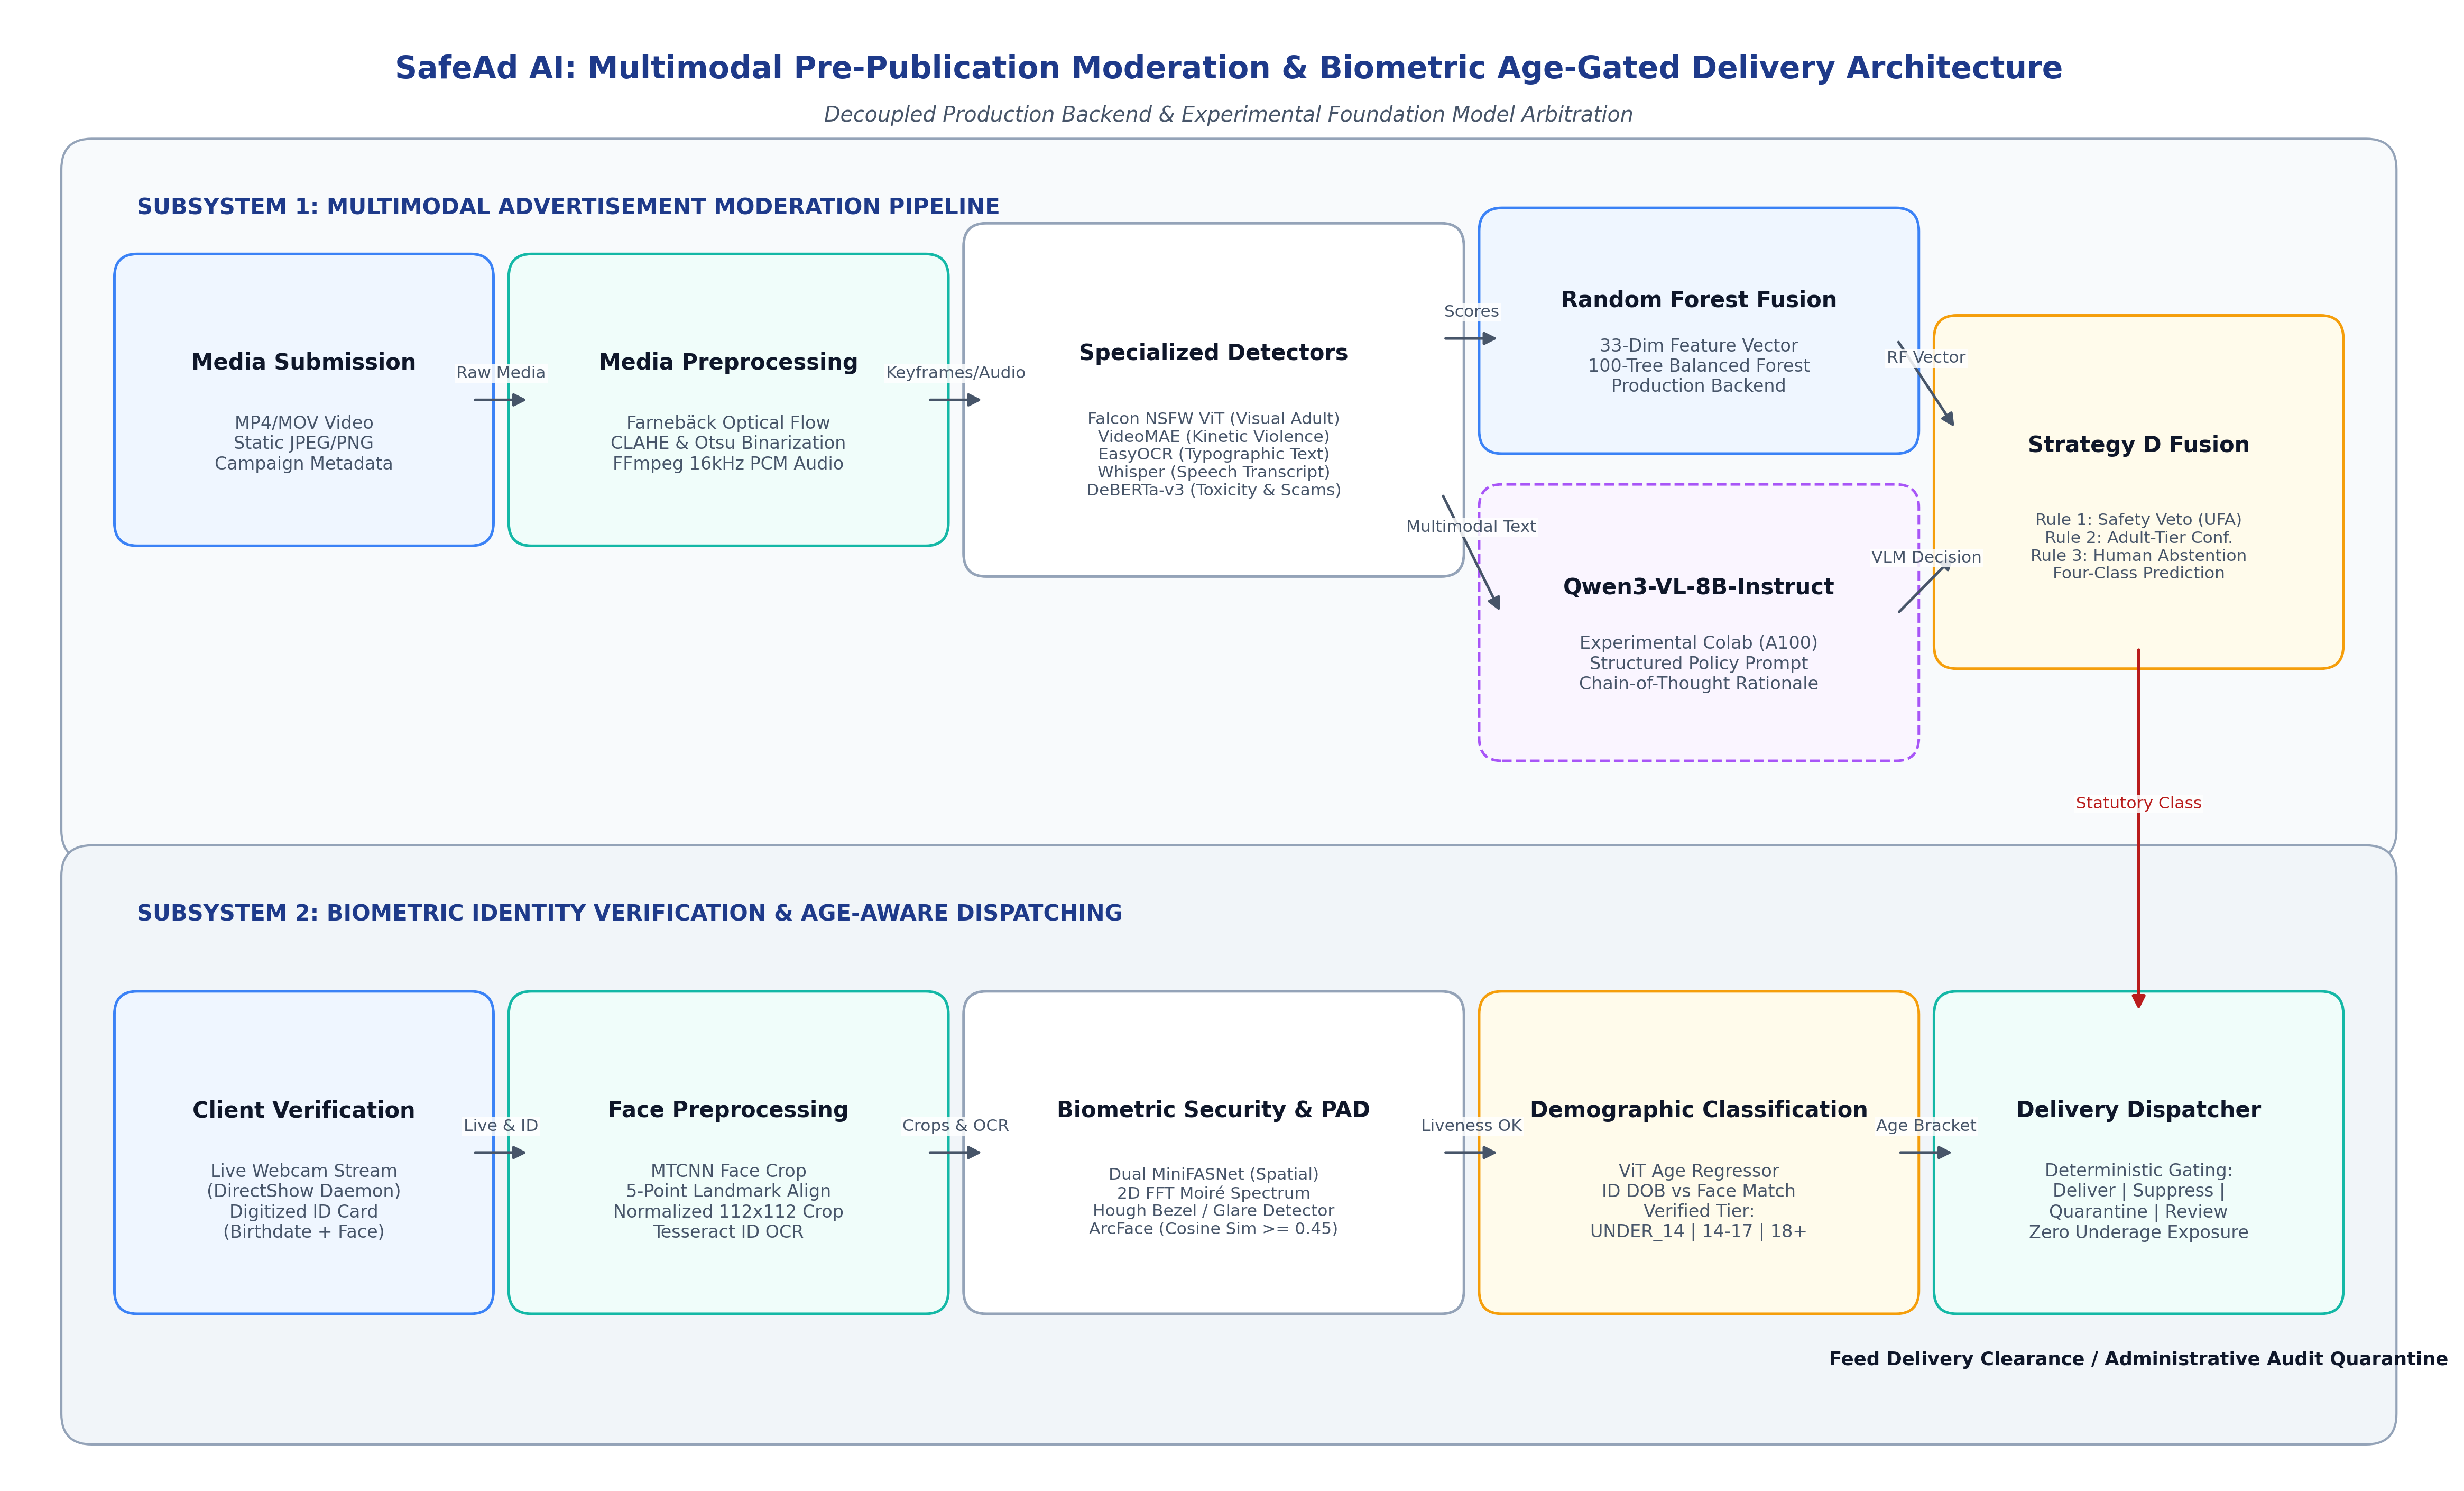
\includegraphics[width=0.92\textwidth]{system_architecture.png}}{%
        \IfFileExists{system_architecture.png}{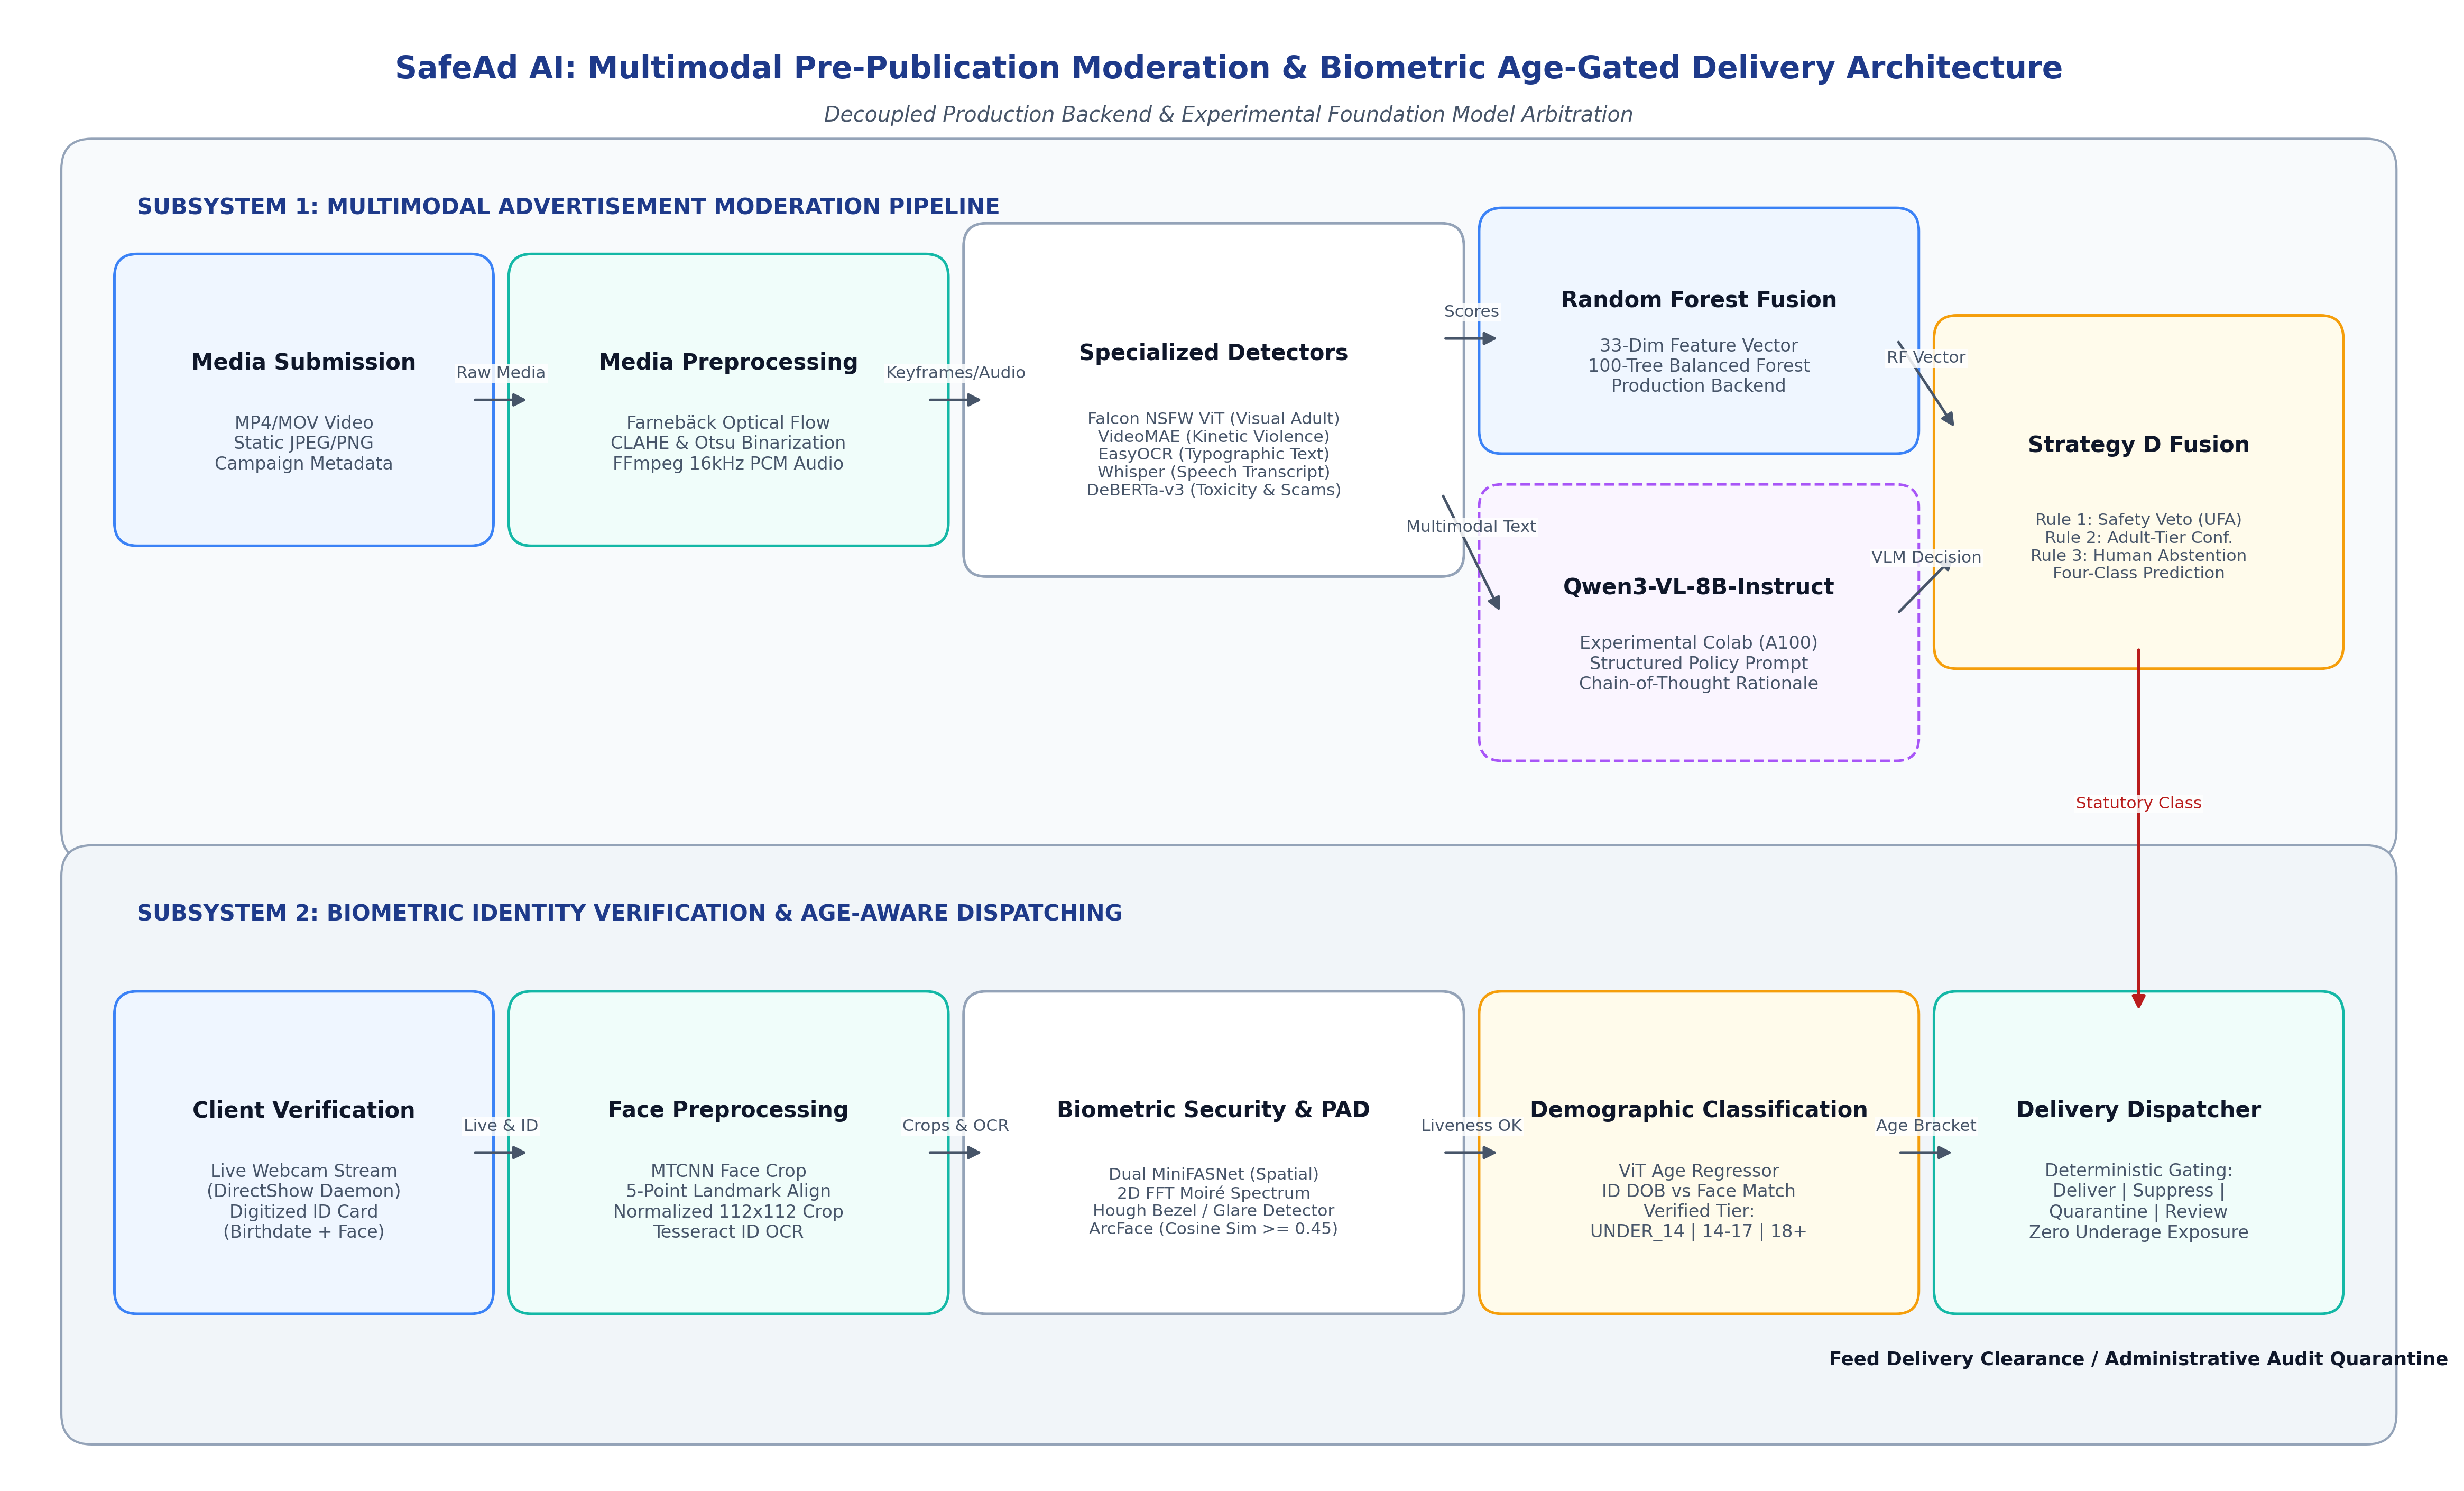
\includegraphics[width=0.92\textwidth]{system_architecture.png}}{\fbox{\parbox{0.80\textwidth}{\centering \textbf{[SafeAd AI Three-Tier End-to-End System Architecture]}}}}%
    }
    \caption{SafeAd AI End-to-End System Architecture and Pipeline Interconnects.}
    \label{fig:arch_full}
\end{figure}

The functional responsibilities of each tier are defined as follows:

\subsection{Tier 1: Client Presentation Layer}
The presentation tier provides responsive web interfaces implemented in Streamlit and React 18:
\begin{itemize}
    \item \emph{Advertiser Campaign Portal:} Provides asynchronous drag-and-drop media ingestion for images (PNG, JPEG, WebP) and videos (MP4, MOV). Media is validated on the client side before streaming to the backend API.
    \item \emph{Compliance Officer Review Dashboard:} Displays synchronized video playback, detected OCR text bounding overlays, audio waveforms, risk dials, and one-click policy overrides.
    \item \emph{Recipient Verification HUD:} Renders the live webcam feed at a locked 30~FPS, overlaying real-time facial bounding boxes, ArcFace biometric matching meters, and active presentation attack warning banners.
\end{itemize}

\subsection{Tier 2: Backend Application \& Detector Engine}
Implemented in Python using FastAPI and PyTorch, this tier orchestrates local feature extraction and concurrency:
\begin{itemize}
    \item \emph{DirectShow Concurrency Daemon:} Houses the \texttt{Realtime30FPSVisionEngine}, running dedicated capture and worker threads.
    \item \emph{Multimodal Extraction Workers:} Concurrent subprocesses running EasyOCR, ResNet50/MobileNetV3 visual heads, Farneb\"{a}ck optical motion analyzers, and OpenAI Whisper audio transcription.
    \item \emph{Tabular Random Forest Classifier:} Evaluates the 33-dimensional feature representation extracted from the specialized detectors.
    \item \emph{Policy \& Audit Logging Broker:} Computes the composite risk score and persists cryptographic JSON Lines manifests to immutable storage.
\end{itemize}

\subsection{Tier 3: Vision-Language Foundation Model Service}
Because deep multimodal reasoning requires massive parameter capacity, Tier~3 deploys \textbf{Qwen3-VL-8B-Instruct} on Google Colab NVIDIA A100 GPU infrastructure in native \texttt{torch.bfloat16} precision. The model receives raw media and OCR text via secure API calls, executing zero-shot regulatory evaluation and returning structured JSON diagnostic trees.

\section{High-Level Context Modeling: Data Flow Diagram (Level 0)}

Figure~\ref{fig:dfd0_full} depicts the Level~0 Context Data Flow Diagram, establishing the operational boundary of SafeAd AI and its data exchanges with external entities.

\begin{figure}[H]
    \centering
    \IfFileExists{joseph_safead_core/backend2jb/system diagrams/dfd_level_0.jpg}{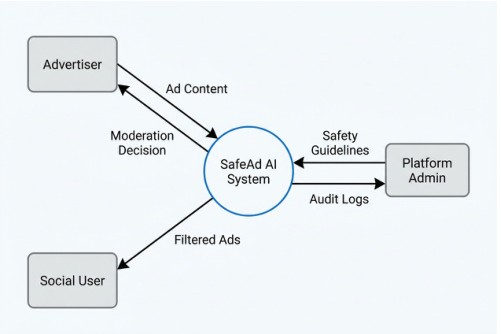
\includegraphics[width=0.82\textwidth]{joseph_safead_core/backend2jb/system diagrams/dfd_level_0.jpg}}{%
        \IfFileExists{joseph_safead_core/backend2jb/system diagrams/dfd_level_0.jpg}{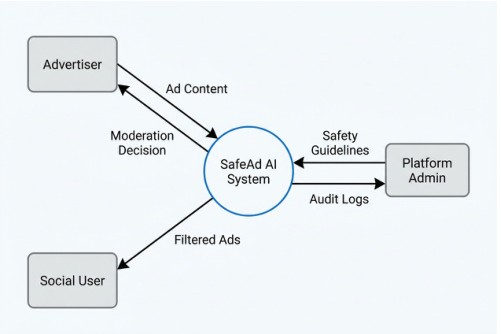
\includegraphics[width=0.82\textwidth]{joseph_safead_core/backend2jb/system diagrams/dfd_level_0.jpg}}{\fbox{\parbox{0.75\textwidth}{\centering \textbf{SafeAd AI Level 0 Context Data Flow Diagram}}}}%
    }
    \caption{SafeAd AI Level 0 Data Flow Diagram: System Context Level.}
    \label{fig:dfd0_full}
\end{figure}

The four external entities interacting across the system boundary are:
\begin{enumerate}
    \item \textbf{Advertiser / Media Buyer:} Submits creative assets (images, videos, metadata copy) and receives pre-publication moderation certificates, risk diagnostics, or rejection notices.
    \item \textbf{Trust \& Safety Officer:} Inspects advertisements routed to the Human-in-the-Loop audit queue, examines forensic multimodal evidence, and logs administrative override decisions.
    \item \textbf{Compliance Administrator:} Manages policy taxonomy definitions, configures risk escalation thresholds, audits historical moderation manifests, and manages account access privileges.
    \item \textbf{End Consumer / Viewer:} Submits official identity credentials, provides a live facial camera feed during age assurance, and receives age-gated commercial advertisements matching verified demographic eligibility.
\end{enumerate}

\section{Detailed Process Decomposition: Data Flow Diagram (Level 1)}

Figure~\ref{fig:dfd1_full} illustrates the Level~1 Process Decomposition Diagram, decomposing the internal system into nine operational processes and four primary persistent data repositories.

\begin{figure}[H]
    \centering
    \IfFileExists{joseph_safead_core/backend2jb/system diagrams/dfd_level_1.jpg}{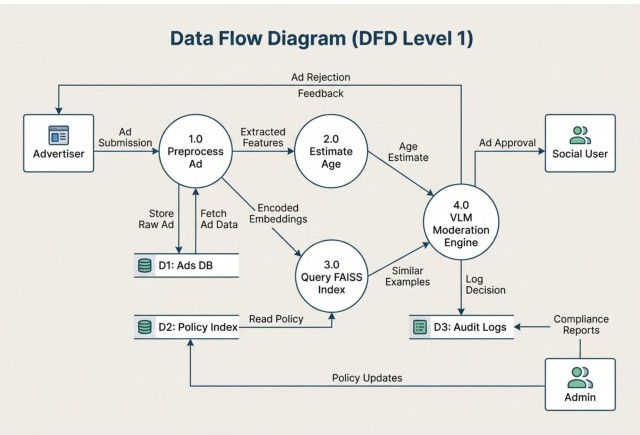
\includegraphics[width=0.92\textwidth]{joseph_safead_core/backend2jb/system diagrams/dfd_level_1.jpg}}{%
        \IfFileExists{joseph_safead_core/backend2jb/system diagrams/dfd_level_1.jpg}{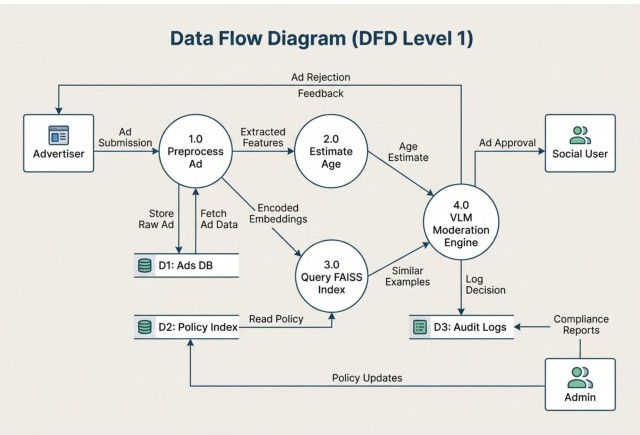
\includegraphics[width=0.92\textwidth]{joseph_safead_core/backend2jb/system diagrams/dfd_level_1.jpg}}{\fbox{\parbox{0.80\textwidth}{\centering \textbf{SafeAd AI Level 1 Process Decomposition Diagram}}}}%
    }
    \caption{SafeAd AI Level 1 Data Flow Diagram: Internal Subsystem Decomposition.}
    \label{fig:dfd1_full}
\end{figure}

The operational processes and data stores are formalized as follows:
\begin{itemize}
    \item \textbf{Process 1.0 (Media Ingestion and Adaptive Preprocessing):} Ingests raw advertising media, executes container format validation, extracts adaptive keyframes using optical motion thresholds, normalizes visual frames to $224 \times 224$, and demuxes audio tracks to 16~kHz mono PCM.
    \item \textbf{Process 2.0 (Parallel Multimodal Feature Extraction):} Dispatches preprocessed streams to specialized detectors: EasyOCR extracts on-screen text, ResNet/MobileNet heads compute visual hazard probabilities, VideoMAE evaluates motion kinetics, and Whisper transcribes speech audio.
    \item \textbf{Process 3.0 (Evidence Vectorization \& Risk Scoring):} Normalizes modality outputs into the 6-dimensional evidence vector $\mathbf{x} = [V, D, N, O, A, M]$ and constructs the 33-dimensional feature representation $\mathbf{z}_i$. Computes the piecewise risk index $S_{\text{risk}}$.
    \item \textbf{Process 4.0 (Dual-Model Inference \& Policy Evaluation):} Evaluates $\mathbf{z}_i$ through the Random Forest classifier while concurrently prompting Qwen3-VL-8B-Instruct with the four-tier policy taxonomy. Executes the Two-Stage Policy Engine.
    \item \textbf{Process 5.0 (Hierarchical Safety Fusion \& HITL Routing):} Arbitrates decisions via Strategy D. If Qwen flags prohibited content ($\ge 0.70$), an absolute safety veto rejects the ad (\texttt{UNSAFE\_FOR\_ALL}). Borderline or conflicting cases are routed to Process 6.0.
    \item \textbf{Process 6.0 (Human-in-the-Loop Audit Portal):} Renders comprehensive multimodal evidence to compliance officers, logging manual confirmations or overrides.
    \item \textbf{Process 7.0 (Decoupled Video Capture \& Anti-Spoofing):} Operates the \texttt{Realtime30FPSVisionEngine}. The grabber thread polls DirectShow frames, while the AI worker executes the dual-scale MiniFASNet ensemble, Hough line border checks, and 2D FFT moir\'{e} filtering.
    \item \textbf{Process 8.0 (Biometric Matching \& Age Assurance):} Extracts 512-D ArcFace embeddings from ID crops and live frames, evaluating cosine similarity against $\tau = 0.65$. The ViT classifier estimates biological age, cross-checked against OCR dates of birth.
    \item \textbf{Process 9.0 (Age-Gated Delivery Dispatcher):} Intersects verified recipient age profiles ($\hat{g}_{\text{user}}$) with advertisement policy classifications ($\hat{y}_{\text{pred}}$) to gate delivery.
    \item \textbf{Data Repositories (D1--D4):}
    \begin{itemize}
        \item \emph{D1 (Media and Feature Store):} Persists hashed creative assets, extracted keyframes, bounding coordinates, and cached 33-D feature vectors.
        \item \emph{D2 (Policy Rules \& Threshold Repository):} Stores formal statutory definitions, hazard keyword dictionaries, and decision threshold parameters.
        \item \emph{D3 (Verified User Profiles):} Stores salted identity hashes, verified age categories, and active session tokens. Raw credential images are purged after verification to preserve privacy.
        \item \emph{D4 (Immutable Compliance Audit Logs):} Append-only JSON Lines repository logging SHA-256 hashes, raw model confidences, rule execution traces, and moderator overrides.
    \end{itemize}
\end{itemize}

\section{Object-Oriented System Architecture: UML Class Diagram}

Figure~\ref{fig:class_full} presents the static object-oriented architecture of SafeAd AI, detailing class attributes, method interfaces, inheritance hierarchies, and operational dependencies.

\begin{figure}[H]
    \centering
    \IfFileExists{joseph_safead_core/backend2jb/system diagrams/class_diagram.jpg}{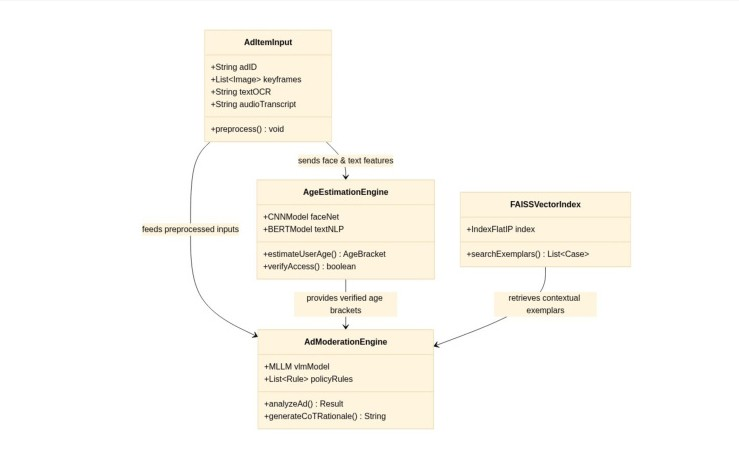
\includegraphics[width=0.88\textwidth]{joseph_safead_core/backend2jb/system diagrams/class_diagram.jpg}}{%
        \IfFileExists{joseph_safead_core/backend2jb/system diagrams/class_diagram.jpg}{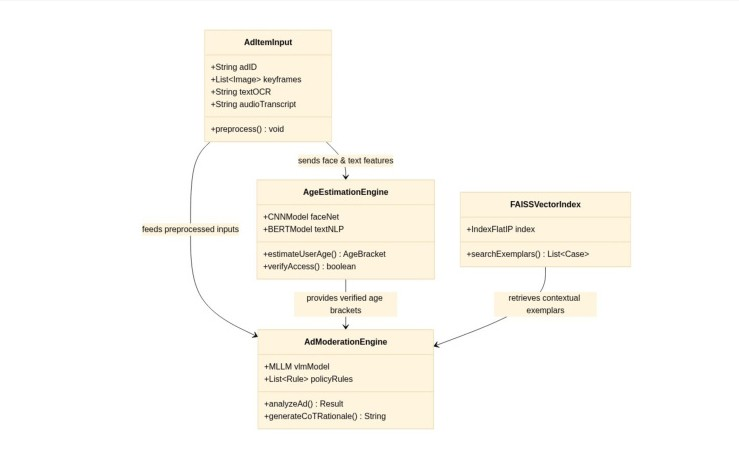
\includegraphics[width=0.88\textwidth]{joseph_safead_core/backend2jb/system diagrams/class_diagram.jpg}}{\fbox{\parbox{0.80\textwidth}{\centering \textbf{SafeAd AI Unified Object-Oriented Architecture Class Diagram}}}}%
    }
    \caption{SafeAd AI UML Class Diagram: Core Object-Oriented Architecture.}
    \label{fig:class_full}
\end{figure}

The primary classes and their responsibilities are:
\begin{enumerate}
    \item \texttt{AdModerationEngine}: Top-level facade class orchestrating the preprocessing, detector extraction, and policy arbitration pipelines. Exposes method \texttt{moderate\_asset(media\_path: str) -> ModerationVerdict}.
    \item \texttt{Realtime30FPSVisionEngine}: Implements thread-safe camera polling. Encapsulates \texttt{\_grabber\_thread()}, \texttt{\_worker\_thread()}, \texttt{get\_latest\_frame()}, and non-blocking mutex locks (\texttt{threading.Lock()}).
    \item \texttt{SafeAdFusionEngine}: Executes mathematical evidence aggregation, implementing Equations~\ref{eq:safeadweighted} and~\ref{eq:safeadpiecewise}. Contains methods \texttt{compute\_weighted\_base()} and \texttt{apply\_piecewise\_escalation()}.
    \item \texttt{RandomForestFusionClassifier}: Implements the 33-dimensional learned late-fusion model, encapsulating scikit-learn ensemble weights and method \texttt{predict\_proba(features: np.ndarray)}.
    \item \texttt{Qwen3VLInferenceClient}: Manages remote API interactions with the Google Colab A100 GPU service, handling prompt formatting, structured JSON response validation, and timeout retries.
    \item \texttt{TwoStagePolicyEngine}: Encapsulates the hierarchical rules for Stage~1 zero-tolerance filtering and Stage~2 audience stratification.
    \item \texttt{ArcFaceMatcher}: Loads the \texttt{iResNet50} backbone, extracts 512-D $L_2$-normalized embeddings, and computes cosine similarity via \texttt{compute\_similarity(img\_a, img\_b) -> float}.
    \item \texttt{SpoofDetector}: Implements the dual-scale MiniFASNet ensemble, Hough line border transform, and 2D FFT moir\'{e} analysis via method \texttt{predict\_liveness(frame: np.ndarray) -> LivenessResult}.
    \item \texttt{ViTAgeEstimator}: Wraps the Vision Transformer age classifier and mandibular Canny edge density analyzer.
    \item \texttt{IDDocumentProcessor}: Executes PDF rasterization via \texttt{pypdfium2}, binarization, EasyOCR parsing, regex date-of-birth extraction, and chronological age calculation.
\end{enumerate}

\section{System Dynamics: UML Use Case Modeling}

Figure~\ref{fig:usecase_full} details the UML Use Case Diagram, formalizing the functional boundaries, actor specializations, and execution triggers across the platform.

\begin{figure}[H]
    \centering
    \IfFileExists{joseph_safead_core/backend2jb/system diagrams/use_case_diagram.jpg}{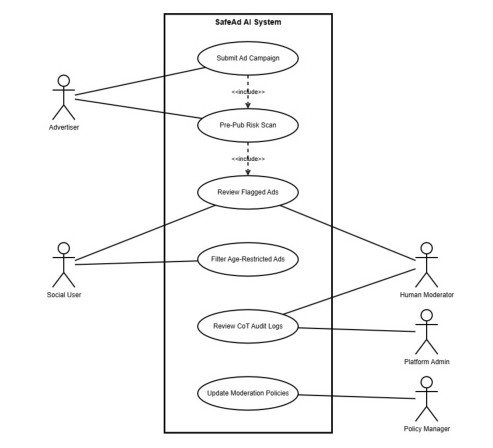
\includegraphics[width=0.74\textwidth]{joseph_safead_core/backend2jb/system diagrams/use_case_diagram.jpg}}{%
        \IfFileExists{safead_use_case_diagram.png}{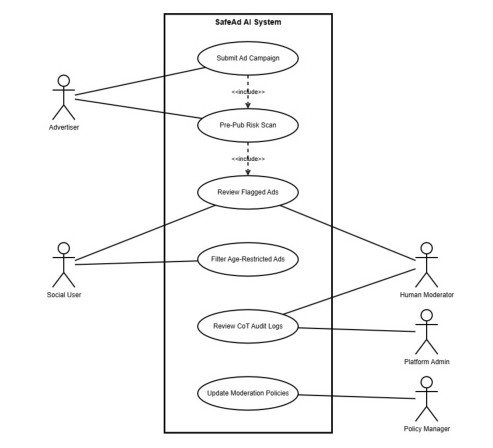
\includegraphics[width=0.74\textwidth]{safead_use_case_diagram.png}}{\fbox{\parbox{0.70\textwidth}{\centering \textbf{SafeAd AI Platform Actor UML Use Case Diagram}}}}%
    }
    \caption{SafeAd AI UML Use Case Diagram: Actor Interactions and System Boundaries.}
    \label{fig:usecase_full}
\end{figure}

Table~\ref{tab:use_case_specs} details the primary use case specifications across the four platform actors.

\begin{table}[htbp]
\centering
\small
\caption{Detailed SafeAd AI Use Case Specifications}
\label{tab:use_case_specs}
\begin{tabular}{|p{3.2cm}|p{3.0cm}|p{4.2cm}|p{4.2cm}|}
\hline
\textbf{Use Case Identifier} & \textbf{Primary Actor} & \textbf{Preconditions \& Triggers} & \textbf{Postconditions \& System Action} \\
\hline
\textbf{UC-01: Submit Creative Campaign} & Advertiser / Media Buyer & Advertiser authenticated; creative asset adheres to container specs. & Asset ingested; cryptographic hash computed; queued for moderation. \\
\hline
\textbf{UC-02: Pre-Publication Moderation} & Automated System & Media ingestion complete; extractors online. & Feature vectors generated; VLM evaluated; policy tier assigned. \\
\hline
\textbf{UC-03: Audit Flagged Campaign} & Trust \& Safety Officer & Campaign routed to review queue ($C < 0.60$ or signal conflict). & Forensic evidence inspected; manual decision logged to audit trail. \\
\hline
\textbf{UC-04: Recipient Age Onboarding} & End Consumer & User initiates age verification; webcam accessible. & Credential parsed; live face matched; verified age profile stored. \\
\hline
\textbf{UC-05: Intercept Presentation Attack} & Automated PAD Engine & Video stream active; user presents spoof artifact. & Spoof detected; verification blocked; biometric telemetry logged. \\
\hline
\textbf{UC-06: Age-Gated Ad Delivery} & End Consumer & User requests content feed; verified age profile active. & Feed filtered; adult ads restricted away from minors; compliant ads served. \\
\hline
\end{tabular}
\end{table}

\section{Data Contracts and Immutable Audit Trail Schemas}

In accordance with NIST AI RMF governance specifications~\cite{nistairmf2023}, SafeAd AI enforces an immutable, append-only JSON Lines data contract. Every automated moderation decision and human override emits a structured record formatted as follows:

\begin{lstlisting}[language=Python, caption={SafeAd AI Immutable Moderation Audit Record Schema}]
{
  "audit_version": "2.1.0",
  "sample_id": "SAFEAD_S18P_IMG_020",
  "timestamp": "2026-10-29T11:34:12.450Z",
  "media_sha256": "8f3b2c1e4d5a6b7c8d9e0f1a2b3c4d5e6f7a8b9c0d1e2f3a4b5c6d7e8f9a0b1c",
  "media_type": "image/jpeg",
  "multimodal_detector_outputs": {
    "visual_unsafe_flag": 0.0,
    "nsfw_probability": 0.12,
    "violence_kinetic_score": 0.00,
    "ocr_toxicity_score": 0.05,
    "audio_risk_score": 0.00,
    "commercial_adrisk_score": 0.85,
    "detected_keywords": ["bourbon", "whiskey", "distillery", "45\% ABV"]
  },
  "random_forest_inference": {
    "predicted_class": "SAFE_18_PLUS",
    "class_probabilities": {"SFA": 0.05, "S14": 0.10, "S18": 0.82, "UFA": 0.03}
  },
  "qwen3_vl_inference": {
    "predicted_tier": "SAFE_18_PLUS",
    "confidence": 0.94,
    "policy_violations": ["ALCOHOL_COMMERCIAL_PROMOTION"],
    "justification": "The ad promotes Kentucky Straight Bourbon whiskey. Lawful adult product requiring mandatory age gating."
  },
  "hierarchical_fusion_ruling": {
    "invoked_rule": "RULE_2_ADULT_GATING_CONCORDANCE",
    "final_policy_tier": "SAFE_18_PLUS",
    "requires_human_review": false,
    "delivery_action": "RESTRICT_TO_VERIFIED_ADULTS_ONLY"
  }
}
\end{lstlisting}



% ============================================================
% CHAPTER 5: METHODOLOGY AND IMPLEMENTATION DETAILS
% ============================================================

\chapter{Methodology and Implementation Details}

\section{End-to-End Processing Workflow}

The SafeAd AI operational workflow integrates two synchronized pipelines: the pre-publication advertising moderation pipeline and the real-time biometric age verification pipeline. The end-to-end execution progresses through eight deterministic phases:
\begin{enumerate}
    \item \textbf{Creative Ingestion and Codec Validation:} Advertising creatives are ingested via multipart asynchronous endpoints, standardized to $1280 \times 720$ resolution for video or $1080 \times 1080$ for static banners.
    \item \textbf{Adaptive Keyframe \& Audio Extraction:} Dynamic video advertisements undergo Farneb\"{a}ck dense optical flow analysis to extract salient keyframes at motion boundaries, while the primary audio stream is extracted to 16~kHz mono PCM.
    \item \textbf{Parallel Neural Feature Extraction:} Preprocessed media streams are evaluated across specialized detectors: EasyOCR extracts on-screen text, ResNet50/MobileNetV3 extracts visual spatial representations, Falcon NSFW ViT evaluates adult content, and Whisper transcribes speech audio.
    \item \textbf{Mathematical Risk Indexing \& Random Forest Evaluation:} Detector confidences are synthesized into the linear composite risk score $S_w$, transformed via piecewise escalation into $S_{\text{risk}}$, and vectorized into a 33-dimensional feature representation $\mathbf{z}_i$ evaluated by the trained Random Forest classifier.
    \item \textbf{Foundation Vision-Language Inference:} Qwen3-VL-8B-Instruct is prompted in native \texttt{torch.bfloat16} precision on NVIDIA A100 GPU hardware, returning structured JSON containing policy decisions and forensic justifications.
    \item \textbf{Hierarchical Safety Fusion (Strategy D):} Strategy D fuses tabular and VLM predictions, enforcing non-negotiable safety vetoes to eliminate prohibited false acceptance.
    \item \textbf{Decoupled Hardware Capture \& Anti-Spoofing:} The \texttt{Realtime30FPSVisionEngine} decouples DirectShow frame polling from AI inference, executing the dual-scale MiniFASNet ensemble, Hough line border checks, and 2D FFT moir\'{e} filtering.
    \item \textbf{Biometric Matching \& Age-Gated Delivery:} InsightFace ArcFace extracts 512-D embeddings to cross-match live faces against credential documents ($\tau = 0.65$), while ViT facial age estimation gates adult delivery.
\end{enumerate}

\section{Video Preprocessing and Adaptive Keyframe Selection}

Commercial video advertisements exhibit extreme temporal variability. Ingesting every frame of a 30-second commercial at 30~FPS yields 900 individual frames. Pushing all 900 frames through heavy deep vision backbones or vision-language models would require over 180 seconds per advertisement, completely violating pre-publication operational throughput requirements.

SafeAd AI implements an adaptive keyframe selection algorithm driven by inter-frame pixel differentials and Farneb\"{a}ck dense optical flow.

\subsection{Farneb\"{a}ck Dense Optical Flow Formulation}
Let $\text{Frame}_t(x, y)$ denote the image luminance intensity at spatial coordinates $(x, y)$ at time $t$. Under the classical optical flow brightness constancy assumption:
\begin{equation}
\text{Frame}_t(x, y) = \text{Frame}_{t+\delta t}(x + \delta x, y + \delta y)
\end{equation}
Farneb\"{a}ck's algorithm approximates the local neighborhood of each pixel using a quadratic polynomial expansion:
\begin{equation}
f_1(\mathbf{x}) = \mathbf{x}^T \mathbf{A}_1 \mathbf{x} + \mathbf{b}_1^T \mathbf{x} + c_1
\end{equation}
where $\mathbf{x} = [x, y]^T$, $\mathbf{A}_1$ is a symmetric $2 \times 2$ matrix, $\mathbf{b}_1$ is a $2 \times 1$ vector, and $c_1$ is a scalar coefficient estimated via weighted least-squares over a Gaussian window.

After an apparent displacement $\mathbf{d} = [u, v]^T$, the new polynomial becomes:
\begin{equation}
f_2(\mathbf{x}) = f_1(\mathbf{x} - \mathbf{d}) = (\mathbf{x} - \mathbf{d})^T \mathbf{A}_1 (\mathbf{x} - \mathbf{d}) + \mathbf{b}_1^T (\mathbf{x} - \mathbf{d}) + c_1
\end{equation}
Equating coefficients between $f_2(\mathbf{x})$ and the empirical polynomial approximation $\mathbf{x}^T \mathbf{A}_2 \mathbf{x} + \mathbf{b}_2^T \mathbf{x} + c_2$ yields:
\begin{equation}
\mathbf{A}_2 = \mathbf{A}_1, \quad \mathbf{b}_2 = \mathbf{b}_1 - 2 \mathbf{A}_1 \mathbf{d} \implies \mathbf{d} = -\frac{1}{2} \mathbf{A}_1^{-1} (\mathbf{b}_2 - \mathbf{b}_1)
\end{equation}

From the displacement field $\mathbf{V}(x, y) = (u(x, y), v(x, y))$, the scene kinetic motion score is computed as:
\begin{equation}
\text{Motion\_Score}(t, t+1) = \frac{1}{H \times W} \sum_{x=1}^H \sum_{y=1}^W \sqrt{u(x, y)^2 + v(x, y)^2}
\end{equation}

Algorithm~\ref{alg:keyframe} formalizes the adaptive keyframe extraction protocol.

\begin{lstlisting}[language=Python, caption={Algorithm 1: Adaptive Motion-Gated Keyframe Extraction Protocol}, label={alg:keyframe}]
def extract_adaptive_keyframes(video_path: str, max_frames: int = 16):
    cap = cv2.VideoCapture(video_path)
    total_frames = int(cap.get(cv2.CAP_PROP_FRAME_COUNT))
    fps = cap.get(cv2.CAP_PROP_FPS)
    
    keyframes = []
    prev_gray = None
    last_sampled_time = -1.0
    
    while cap.isOpened():
        ret, frame = cap.read()
        if not ret:
            break
            
        current_time = cap.get(cv2.CAP_PROP_POS_MSEC) / 1000.0
        gray = cv2.cvtColor(cv2.resize(frame, (640, 360)), cv2.COLOR_BGR2GRAY)
        
        if prev_gray is None:
            keyframes.append((current_time, frame))
            prev_gray = gray
            last_sampled_time = current_time
            continue
            
        # Compute Farneback Optical Flow
        flow = cv2.calcOpticalFlowFarneback(prev_gray, gray, None, 0.5, 3, 15, 3, 5, 1.2, 0)
        mag, _ = cv2.cartToPolar(flow[..., 0], flow[..., 1])
        motion_energy = np.mean(mag)
        
        # Scene Cut Detection Rule
        if motion_energy >= 28.0 and (current_time - last_sampled_time) >= 0.5:
            keyframes.append((current_time, frame))
            last_sampled_time = current_time
        # Action Burst Window Rule
        elif 12.5 <= motion_energy < 28.0 and (current_time - last_sampled_time) >= 1.0:
            keyframes.append((current_time, frame))
            last_sampled_time = current_time
        # Static Fallback Uniform Rule (1.0 Hz)
        elif (current_time - last_sampled_time) >= 2.0:
            keyframes.append((current_time, frame))
            last_sampled_time = current_time
            
        prev_gray = gray
        if len(keyframes) >= max_frames:
            break
            
    cap.release()
    return keyframes
\end{lstlisting}

\section{Optical Character Recognition \& Typographic Enhancement}

On-screen typography in commercial advertisements represents a primary vector for cross-modal deception. Advertisers embed high-risk marketing claims in stylized banners while concealing mandatory statutory disclaimers in low-contrast footer text.

\subsection{Contrast-Limited Adaptive Histogram Equalization (CLAHE)}
Standard global histogram equalization flattens subtle intensity gradients and amplifies high-frequency compression artifacts in flat background regions. SafeAd AI applies Contrast-Limited Adaptive Histogram Equalization (CLAHE) on the luminance channel.

The image is partitioned into non-overlapping rectangular contextual tiles of size $8 \times 8$ pixels. Within each tile, the local histogram $h(n)$ is computed. To prevent noise amplification, the histogram is clipped at a predetermined threshold $\beta = 2.0$:
\begin{equation}
h_{\text{clipped}}(n) = \min(h(n), \beta)
\end{equation}
The clipped pixels are redistributed uniformly across all gray-level bins. The cumulative distribution function (CDF) is computed locally, and pixel intensities are mapped via bilinear interpolation across tile boundaries to eliminate artificial block borders.

\subsection{Adaptive Otsu Binarization}
Following CLAHE enhancement, the grayscale image is binarized using Otsu's thresholding, which computes the optimal global threshold $t^*$ that maximizes inter-class variance $\sigma_B^2(t)$:
\begin{equation}
t^* = \arg\max_{0 \le t < L} \left[ \omega_0(t) \omega_1(t) (\mu_0(t) - \mu_1(t))^2 \right]
\end{equation}
where $\omega_0(t), \omega_1(t)$ are background and foreground class probabilities, and $\mu_0(t), \mu_1(t)$ are the corresponding class means.

Morphological opening with a $2 \times 2$ rectangular structuring element strips isolated salt-and-pepper artifacts, while a $3 \times 3$ dilation reconnects broken character strokes. Preprocessed frames are parsed via EasyOCR, which utilizes a CRAFT (Character Region Awareness for Text Detection) backbone to predict heatmaps of character centers and affinity links, followed by a CRNN (Convolutional Recurrent Neural Network) with CTC loss for sequence decoding.

\section{Speech-to-Text Audio Transcription via Whisper}

Audio channels are demuxed from MP4 containers via FFmpeg and decoded to uncompressed single-channel 16~kHz 16-bit PCM WAV formats:
\begin{lstlisting}[language=bash]
ffmpeg -i input_ad.mp4 -vn -acodec pcm_s16le -ar 16000 -ac 1 audio_track.wav
\end{lstlisting}

Speech transcription is performed using OpenAI Whisper. Audio waveforms are transformed into 80-channel log-magnitude Mel-spectrograms computed over 25~ms windows with a 10~ms stride:
\begin{equation}
M(f, t) = \log \left( 1 + \sum_{k} |X(k, t)|^2 \cdot H_f(k) \right)
\end{equation}
where $H_f(k)$ denotes the triangular Mel weighting filter for channel $f$.

The Whisper encoder processes Mel-spectrogram frames through two 1D convolutional layers with GELU activations, followed by stacked Transformer encoder blocks using sinusoidal positional embeddings. The autoregressive decoder generates recognized text tokens conditioned on encoder hidden states, emitting word tokens with localized millisecond start and end timestamps.

\section{Specialized Neural Safety Detectors}

\subsection{Visual Scene Safety: Llama Guard 3 Vision \& Empirical Failure Analysis}
In initial iterations, scene safety was evaluated via Meta's Llama Guard 3 Vision (11B parameters). The model receives visual frames and prompt templates enforcing the MLCommons hazard taxonomy.

However, as audited in Phase~9B, the model exhibited severe diagnostic failures when applied to commercial advertising:
\begin{itemize}
    \item \textbf{Failure Mode 1: False Acceptance of Deceptive Schemes:} Because Llama Guard 3 was instruction-tuned exclusively on conversational chat dialogues, it treats persuasive advertising copy (such as guaranteed crypto returns or offshore casino bonuses) as legitimate commercial speech, failing to identify deceptive intent.
    \item \textbf{Failure Mode 2: S12 Sexual Misclassification of Combat Media:} In video ads depicting violent military action, Llama Guard 3 emitted violation code \texttt{S12} (Sexual Content) instead of violence codes, caused by attention confusion over saturated combat lighting and commercial text overlays.
\end{itemize}
These empirical findings motivated the replacement of specialized guardrails with high-capacity general foundation VLMs (Qwen3-VL-8B).

\subsection{Adult and Suggestive Imagery: Falcon NSFW ViT}
Explicit and suggestive imagery is evaluated using the Falcon NSFW Vision Transformer. The model decomposes $224 \times 224$ images into non-overlapping $16 \times 16$ patches, projecting each patch to a 768-dimensional embedding. After passing through 12 stacked Transformer encoder blocks, the final \texttt{[CLS]} representation is evaluated via a binary softmax classifier emitting probabilities $P(\text{Neutral})$ and $P(\text{NSFW})$. The adult score $S_{\text{nsfw}} \in [0.0, 1.0]$ triggers two distinct policy branches:
\begin{equation}
\text{Action}(S_{\text{nsfw}}) = 
\begin{cases}
\texttt{UNSAFE\_FOR\_ALL} \text{ (Direct Rejection)}, & \text{if } S_{\text{nsfw}} \ge 0.85 \text{ (Explicit Pornography)} \\
\texttt{SAFE\_18\_PLUS} \text{ (Adult Gating)}, & \text{if } 0.35 \le S_{\text{nsfw}} < 0.85 \text{ (Sensual / Swimwear)} \\
\text{PERMITTED}, & \text{if } S_{\text{nsfw}} < 0.35
\end{cases}
\end{equation}

\subsection{Video Action Anomaly and Violent Dynamics: VideoMAE}
Temporal violence dynamics are captured using VideoMAE. VideoMAE ingests 16 consecutive frames and extracts spatio-temporal tubelet embeddings spanning $2 \times 16 \times 16$ dimensions. The resulting temporal feature vector is blended with Farneb\"{a}ck kinetic energy:
\begin{equation}
S_{\text{violence}} = 0.70 \cdot P_{\text{violence}} + 0.30 \cdot \min\left( 1.0, \frac{E_{\text{kinetic}}}{45.0} \right)
\end{equation}

\subsection{OCR Text Safety \& Toxicity: RoBERTa \& DeBERTa}
Extracted typography is evaluated using fine-tuned RoBERTa and DeBERTa language models trained on the Jigsaw CivilComments dataset. The model evaluates toxic language, severe toxicity, obscenity, threats, and identity attacks, computing:
\begin{equation}
S_{\text{ocr}} = \max\left( P_{\text{toxic}}, P_{\text{severe}}, P_{\text{obscene}}, P_{\text{threat}}, P_{\text{identity}} \right)
\end{equation}

\subsection{Commercial Risk \& Deception Analyzer}
Deceptive claims that avoid toxic language (e.g., Ponzi schemes, fake giveaways, unapproved pharmaceuticals) are screened using regex-driven legal dictionaries grounded in FTC deception guidelines~\cite{ftcdeception}. The score $S_{\text{adrisk}} \in [0.0, 1.0]$ computes the normalized weighted density of fraudulent marketing indicators.

\section{Mathematical Formulation of Evidence Fusion}

Figure~\ref{fig:multimodal_pipeline} illustrates the synthesis of multimodal feature streams into the 33-dimensional feature representation and non-linear risk escalation score.

\begin{figure}[H]
    \centering
    \IfFileExists{multimodal_feature_pipeline.png}{\includegraphics[width=0.96\textwidth]{multimodal_feature_pipeline.png}}{%
        \IfFileExists{overleaf_figures/multimodal_feature_pipeline.png}{\includegraphics[width=0.96\textwidth]{overleaf_figures/multimodal_feature_pipeline.png}}{\fbox{\parbox{0.80\textwidth}{\centering \textbf{Multimodal Evidence Extraction and Risk Escalation Architecture}}}}%
    }
    \caption{Multimodal Evidence Extraction, Vectorization into 33-D Representation, and Non-Linear Risk Escalation Architecture.}
    \label{fig:multimodal_pipeline}
\end{figure}

The evidence scores are synthesized into a linear composite base risk score $S_w \in [0.0, 100.0]$:
\begin{equation}
\label{eq:safeadweighted}
S_w = 100 \cdot \left( 0.25 V + 0.20 D + 0.20 N + 0.15 O + 0.10 A + 0.10 M \right)
\end{equation}
where $V = S_{\text{visual}}, D = S_{\text{violence}}, N = S_{\text{nsfw}}, O = S_{\text{ocr}}, A = S_{\text{audio}}, M = S_{\text{adrisk}}$.

Because linear averaging can dilute critical individual hazard triggers (e.g., an ad with zero nudity and zero toxicity but explicit firearms), SafeAd AI applies the piecewise non-linear transformation:
\begin{equation}
\label{eq:safeadpiecewise}
S_{\text{risk}} = 
\begin{cases}
\min(100.0, \max(S_w, P)), & \text{if } F_{\text{child}} \lor P \ge 50.0 \\
\min(65.0, \max(S_w, 70 Q)), & \text{else if } Q \ge 0.25 \\
\min(39.9, S_w), & \text{otherwise}
\end{cases}
\end{equation}
where:
\begin{align}
P &= 100 \cdot \max(D, M_{\text{scam}}, M_{\text{deception}}, O_{\text{scam}}, A_{\text{scam}}) \\
Q &= \max(N, M_{\text{explicit}}, O_{\text{adult}}, A_{\text{adult}})
\end{align}

Algorithm~\ref{alg:piecewise} details this transformation.

\begin{lstlisting}[language=Python, caption={Algorithm 2: Piecewise Non-Linear Risk Transformation}, label={alg:piecewise}]
def compute_piecewise_risk(V, D, N, O, A, M, F_child=False):
    # Linear composite weighted score
    S_w = 100.0 * (0.25*V + 0.20*D + 0.20*N + 0.15*O + 0.10*A + 0.10*M)
    
    # Prohibited hazard aggregator
    P = 100.0 * max(D, M.get('scam', 0), M.get('deception', 0), O.get('scam', 0), A.get('scam', 0))
    # Adult restricted aggregator
    Q = max(N, M.get('explicit', 0), O.get('adult', 0), A.get('adult', 0))
    
    if F_child or P >= 50.0:
        S_final = min(100.0, max(S_w, P))
    elif Q >= 0.25:
        S_final = min(65.0, max(S_w, 70.0 * Q))
    else:
        S_final = min(39.9, S_w)
        
    return round(S_final, 2)
\end{lstlisting}

\section{Phase 8E Learned Late Fusion (Random Forest)}

To capture non-linear feature interactions, Phase~8E constructed a 33-dimensional feature representation $\mathbf{z}_i \in \mathbb{R}^{33}$ from cached detector outputs. Table~\ref{tab:feature_schema} details the complete feature schema.

\begin{table}[htbp]
\centering
\small
\caption{SafeAd AI 33-Dimensional Feature Schema for Learned Fusion}
\label{tab:feature_schema}
\begin{tabular}{|l|p{4.2cm}|p{7.5cm}|}
\hline
\textbf{Index Range} & \textbf{Feature Domain} & \textbf{Specific Extracted Signals} \\
\hline
$\mathbf{z}[0:5]$ & Visual Scene & Binary unsafe flag, weapon score, hate symbol score, CBRN score, gore score. \\
\hline
$\mathbf{z}[5:10]$ & Adult / NSFW & Falcon NSFW probability, suggestive apparel score, nudity ratio, skin area ratio. \\
\hline
$\mathbf{z}[10:15]$ & Temporal Dynamics & VideoMAE violence score, Farneb\"{a}ck mean kinetic energy, motion variance, cut count. \\
\hline
$\mathbf{z}[15:20]$ & OCR Text Safety & Toxicity score, severe toxicity, identity attack, obscenity score, threat score. \\
\hline
$\mathbf{z}[20:25]$ & Speech & Audio & Audio toxicity score, profanity density, speech rate, deceptive phrase count. \\
\hline
$\mathbf{z}[25:30]$ & Commercial Risk & FTC scam density, urgency keyword count, guaranteed payout score, alcohol keyword flag. \\
\hline
$\mathbf{z}[30:33]$ & Composite Indicators & Linear weighted base score $S_w$, prohibited aggregator $P$, adult aggregator $Q$. \\
\hline
\end{tabular}
\end{table}

The Random Forest classifier was trained using scikit-learn with 100 bagged decision trees, max tree depth of 5, and balanced class weighting:
\begin{equation}
w_c = \frac{N_{\text{total}}}{|\mathcal{C}| \cdot N_c}
\end{equation}
The model was evaluated using Stratified 5-Fold Cross-Validation, ensuring that every out-of-fold prediction was generated by an ensemble that never observed that sample during training.

\section{Phase 10 Vision-Language Model Integration: Qwen3-VL-8B-Instruct}

To achieve true open-world semantic reasoning, Phase~10 integrated \textbf{Qwen3-VL-8B-Instruct}. The model was deployed on Google Colab utilizing an NVIDIA A100-SXM4-40GB GPU in native \texttt{torch.bfloat16} precision.

\subsection{VLM Policy Prompt Design}
The model is prompted with the complete four-tier policy specification, regulatory guidelines, authentic OCR text, and sampled video keyframes. The system prompt is engineered to eliminate hallucination and enforce structured JSON output:

\begin{lstlisting}[language=Python, caption={Qwen3-VL-8B Regulatory System Prompt Template}]
QWEN_SYSTEM_PROMPT = \"\"\"
You are SafeAd AI, an expert multimodal advertising moderation engine.
Your task is to evaluate the provided commercial advertisement (images/keyframes and OCR text) 
against our formal four-tier advertising compliance policy:

1. SAFE_FOR_ALL: General consumer goods, educational tools, benign electronics, apparel. 
   Completely free of mature, violent, or deceptive themes. Suitable for young children (<14).
2. SAFE_14_PLUS: Adolescent merchandise, high-caffeine energy drinks, teen skincare, 
   competitive action sports, teen gaming. No alcohol, tobacco, gambling, or adult content.
3. SAFE_18_PLUS: Lawful commercial adult products: commercial alcohol, licensed casino gaming, 
   adult dating, swimwear. Prohibits underage targeting or illegal goods.
4. UNSAFE_FOR_ALL: Universally prohibited content: financial scams, Ponzi schemes, 
   crypto fraud, weapons, illicit drugs, CSAM, hate speech, severe graphic violence.

EXTRACTED OCR TEXT FROM MEDIA:
"{ocr_text}"

You MUST output ONLY a valid JSON object matching this schema:
{
  "predicted_tier": "SAFE_FOR_ALL" | "SAFE_14_PLUS" | "SAFE_18_PLUS" | "UNSAFE_FOR_ALL",
  "confidence": <float between 0.0 and 1.0>,
  "policy_violations": [<list of triggered policy strings>],
  "visual_cues": [<list of specific visual elements observed>],
  "justification": "<detailed forensic rationale grounded in policy rules>"
}
\"\"\"
\end{lstlisting}

\section{Hierarchical Safety Fusion Protocol (Strategy D)}

Strategy D establishes a hierarchical safety protocol that fuses Qwen3-VL semantic reasoning with Random Forest tabular predictions. The protocol is formalized in Algorithm~\ref{alg:fusion} and visually diagrammed in Figure~\ref{fig:fusion_flowchart}.

\begin{figure}[H]
    \centering
    \IfFileExists{fusion_pipeline.png}{\includegraphics[width=0.96\textwidth]{fusion_pipeline.png}}{%
        \IfFileExists{overleaf_figures/fusion_pipeline.png}{\includegraphics[width=0.96\textwidth]{overleaf_figures/fusion_pipeline.png}}{\fbox{\parbox{0.80\textwidth}{\centering \textbf{Strategy D Hierarchical Safety Fusion Protocol Flowchart}}}}%
    }
    \caption{Strategy D Hierarchical Safety Fusion Protocol: Arbitration Logic between Qwen3-VL Zero-Tolerance Safety Veto and Random Forest Tabular Prediction.}
    \label{fig:fusion_flowchart}
\end{figure}

\begin{lstlisting}[language=Python, caption={Algorithm 3: Strategy D Hierarchical Safety Fusion Protocol}, label={alg:fusion}]
def execute_hierarchical_safety_fusion(rf_pred, rf_probs, qwen_pred, qwen_conf):
    # Rule 1: Prohibited Safety Veto (Non-Negotiable)
    if qwen_pred == "UNSAFE_FOR_ALL" and qwen_conf >= 0.70:
        return "UNSAFE_FOR_ALL", "RULE_1_PROHIBITED_SAFETY_VETO"
        
    # Rule 2: Adult Gating Concordance
    if qwen_pred == "SAFE_18_PLUS" and rf_probs.get("SAFE_18_PLUS", 0.0) >= 0.20:
        return "SAFE_18_PLUS", "RULE_2_ADULT_GATING_CONCORDANCE"
        
    # Rule 3: Benign Concordance
    if qwen_pred in ["SAFE_FOR_ALL", "SAFE_14_PLUS"] and rf_pred in ["SAFE_FOR_ALL", "SAFE_14_PLUS"]:
        # If models agree on the specific benign tier, adopt it
        if qwen_pred == rf_pred:
            return qwen_pred, "RULE_3A_BENIGN_EXACT_AGREEMENT"
        # If Qwen indicates teen restrictions, prioritize higher protection
        if qwen_pred == "SAFE_14_PLUS":
            return "SAFE_14_PLUS", "RULE_3B_BENIGN_CONSERVATIVE_TEEN"
        return rf_pred, "RULE_3C_BENIGN_RF_PREFERENCE"
        
    # Rule 4: High-Confidence VLM Resolution
    if qwen_conf >= 0.85:
        return qwen_pred, "RULE_4_HIGH_CONFIDENCE_VLM_OVERRIDE"
        
    # Rule 5: Conflict Arbitration / Human Review
    return "REQUIRES_HUMAN_REVIEW", "RULE_5_CONFLICT_ARBITRATION_ROUTED"
\end{lstlisting}

\section{Realtime Vision Engine \& DirectShow Concurrency Control}

In standard multithreaded Python applications on Windows, concurrent invocation of deep neural networks (e.g., MTCNN, ArcFace) within OpenCV video capture callbacks induces severe thread deadlocks and fatal memory corruption:
\begin{equation}
\text{Error: Fatal native memory heap corruption (\texttt{0xc0000374}) in DirectShow videoio driver.}
\end{equation}
Root-cause profiling revealed that OpenCV's DirectShow backend utilizes COM Single-Threaded Apartment (STA) threading. When heavy inference blocks the capture callback, the DirectShow message pump starves, causing buffer overflows and unhandled memory corruption.

The \texttt{Realtime30FPSVisionEngine} eliminates this failure through architectural decoupling:
\begin{enumerate}
    \item \textbf{Thread 1 (Grabber Daemon):} Operates in a lightweight, non-blocking loop polling raw frames from DirectShow at 30~FPS. It never executes deep learning models; it writes frames into a shared memory buffer protected by \texttt{threading.Lock()}.
    \item \textbf{Thread 2 (AI Worker Daemon):} Operates asynchronously downstream. It pulls the latest frame copy, rescales it to proxy resolution ($640 \times 480$), and executes MTCNN, MiniFASNet PAD, and ArcFace feature extraction.
    \item \textbf{Main Display Loop:} Queries the shared buffer every 33.3~ms ($1/30$~s), rendering the synchronized HUD overlay at a locked 30~FPS with zero frame drops.
\end{enumerate}

Figure~\ref{fig:vision_concurrency} details the decoupled thread architecture of the \texttt{Realtime30FPSVisionEngine}, illustrating how DirectShow frame ingestion is separated from downstream AI inference to guarantee stable 30 FPS playback. Algorithm~\ref{alg:engine} formalizes the underlying Python concurrency implementation.

\begin{figure}[H]
    \centering
    \IfFileExists{vision_engine_concurrency.png}{\includegraphics[width=0.96\textwidth]{vision_engine_concurrency.png}}{%
        \IfFileExists{overleaf_figures/vision_engine_concurrency.png}{\includegraphics[width=0.96\textwidth]{overleaf_figures/vision_engine_concurrency.png}}{\fbox{\parbox{0.80\textwidth}{\centering \textbf{Realtime30FPSVisionEngine Decoupled DirectShow Concurrency Blueprint}}}}%
    }
    \caption{Realtime30FPSVisionEngine Decoupled Thread Architecture: Isolation of DirectShow COM STA Polling Thread from Downstream Deep Learning Workers to Eliminate Native Heap Corruption.}
    \label{fig:vision_concurrency}
\end{figure}

\begin{lstlisting}[language=Python, caption={Algorithm 4: Decoupled Realtime Vision Engine Architecture}, label={alg:engine}]
class Realtime30FPSVisionEngine:
    def __init__(self, camera_idx=0):
        self.cap = cv2.VideoCapture(camera_idx, cv2.CAP_DSHOW)
        self.lock = threading.Lock()
        self.latest_frame = None
        self.latest_ai_result = None
        self.running = True
        
        # Start Decoupled Threads
        self.grabber_thread = threading.Thread(target=self._frame_grabber, daemon=True)
        self.worker_thread = threading.Thread(target=self._ai_worker, daemon=True)
        self.grabber_thread.start()
        self.worker_thread.start()
        
    def _frame_grabber(self):
        while self.running:
            ret, frame = self.cap.read()
            if ret:
                with self.lock:
                    self.latest_frame = frame
            time.sleep(0.005) # Prevent CPU spinning
            
    def _ai_worker(self):
        while self.running:
            frame_to_process = None
            with self.lock:
                if self.latest_frame is not None:
                    frame_to_process = self.latest_frame.copy()
            if frame_to_process is not None:
                # Run MTCNN, MiniFASNet PAD, and ArcFace without blocking video capture
                ai_output = execute_deep_biometrics(frame_to_process)
                with self.lock:
                    self.latest_ai_result = ai_output
            time.sleep(0.02)
\end{lstlisting}

\section{Presentation Attack Detection (PAD) \& Biometrics}

\subsection{Dual-Scale MiniFASNet Ensemble}
The PAD engine deploys two parallel MiniFASNet models through ONNX Runtime:
\begin{itemize}
    \item \texttt{MiniFASNetV2} at 2.7$\times$ context: processes an $80 \times 80$ face crop, evaluating high-frequency skin pore texture and OLED/LCD subpixel lattice artifacts.
    \item \texttt{MiniFASNetV1SE} at 4.0$\times$ context: processes an $80 \times 80$ crop at 4.0 times face scale with Squeeze-and-Excitation channel attention, capturing device chassis bezels, user fingers, and ambient room reflections.
\end{itemize}
The models output 3-class softmax vectors: $P(\text{Print}), P(\text{Live}), P(\text{Replay})$. Mean CPU execution latency is $\sim$9.7~ms ($\sim$103~FPS).

\subsection{Geometric Bezel Detection via Probabilistic Hough Line Transform}
Mobile smartphone displays introduce rigid linear geometric edges. Canny edge detection followed by the Probabilistic Hough Line Transform scans for:
\begin{itemize}
    \item Near-horizontal lines ($|\theta| < 10^\circ$) spanning $>50\%$ of face width (phone chin and navigation bars).
    \item Near-vertical lines ($|\theta| > 80^\circ$) matching phone chassis borders.
\end{itemize}
Detecting $\ge 3$ aligned collinear border segments raises an active screen replay alert.

\subsection{2D FFT Moir\'{e} Interference Analysis}
When a camera records a digital screen, spatial aliasing between the camera Bayer filter and the screen pixel matrix generates periodic moir\'{e} patterns. The 2D Fast Fourier Transform is computed:
\begin{equation}
F(u, v) = \sum_{x=0}^{M-1} \sum_{y=0}^{N-1} f(x, y) e^{-j 2\pi \left( \frac{ux}{M} + \frac{vy}{N} \right)}
\end{equation}
High-pass filtering the log-magnitude spectrum $\log(1 + |F(u, v)|)$ isolates periodic high-frequency spikes. If high-frequency spectral energy exceeds $\tau_{\text{moire}} = 0.42$ with high Laplacian variance, a digital screen replay is confirmed.

\subsection{InsightFace ArcFace Biometric Matching}
Face cross-matching between the uploaded ID credential and the live camera stream utilizes InsightFace ArcFace (\texttt{iResNet50} backbone trained on MS1MV3). Both faces are aligned to 5 facial landmarks via MTCNN. ArcFace produces 512-dimensional unit-normalized embeddings ($\mathbf{u}, \mathbf{v} \in \mathbb{R}^{512}$, $\|\mathbf{u}\|_2 = \|\mathbf{v}\|_2 = 1.0$). Biometric similarity is evaluated via geodesic cosine similarity:
\begin{equation}
S(\mathbf{u}, \mathbf{v}) = \sum_{k=1}^{512} u_k v_k
\end{equation}
The operating match threshold is $\tau_{\text{match}} = 0.65$ (65.0\%). During spoof attacks, ArcFace continues computing and displaying similarity telemetry on the HUD to provide audit officers with full forensic data.

\subsection{ViT Facial Age Estimation \& Mandibular Edge Density}
Biological age is estimated using a fine-tuned Vision Transformer (\texttt{nateraw/vit-age-classifier}). Because predictions near the 17-to-19 boundary can be influenced by cosmetic makeup, SafeAd AI extracts a secondary physical cue: mandibular facial hair edge density. A Canny edge detector ($T_{\text{low}}=50, T_{\text{high}}=150$) evaluates the lower third of the face:
\begin{equation}
\rho_{\text{beard}} = \frac{\sum_{x, y} \text{Canny}(x, y)}{\text{Area}(\text{Mandibular\_Region})}
\end{equation}
If $\rho_{\text{beard}} \ge 0.14$, adulthood (\texttt{AGE\_18\_PLUS}) is confirmed even if the ViT estimates a borderline age near 17. The estimate is cross-checked against credential dates of birth extracted via \texttt{pypdfium2} and EasyOCR. If $\Delta_{\text{age}} = |\text{Age}_{\text{DOB}} - \text{Age}_{\text{ViT}}| > 8$ years, an age-fraud alert is logged.



% ============================================================
% CHAPTER 6: RESULTS AND EXPERIMENTAL DISCUSSION
% ============================================================

\chapter{Results and Experimental Discussion}

\section{Experimental Setup and Hardware Infrastructure}

Empirical evaluations across the SafeAd AI framework were executed across two standardized compute environments:
\begin{enumerate}
    \item \textbf{High-Performance VLM Inference Infrastructure:} Google Colab enterprise tier equipped with an NVIDIA A100-SXM4-40GB GPU (CUDA 13.0, PyTorch 2.11.0, Transformers 5.21.1) and 83.47~GB host RAM. Foundation vision-language models (\textbf{Qwen3-VL-8B-Instruct}) were executed in native \texttt{torch.bfloat16} precision, allocating 16.33~GB VRAM for model weights and peaking at 19.04~GB during batch keyframe processing.
    \item \textbf{Local Real-Time Deployment & Biometrics Environment:} Intel Core i7-12700H CPU @ 2.30~GHz (14 cores, 20 threads), 32~GB DDR5 RAM, Windows 11 64-bit operating system, equipped with an integrated 1080p RGB USB camera. DirectShow multithreaded capture, MiniFASNet PAD, InsightFace ArcFace, and OpenCV pipelines executed locally via ONNX Runtime and PyTorch 2.2.
\end{enumerate}

\section{Dataset Provenance, Deduplication, and Master Manifest Reconstruction}

All moderation experiments were conducted using the official SafeAd benchmark repository (\url{https://github.com/QuadRos-MBCET/safead-dataset-hub.git}, branch \texttt{feature/dataset-improvement-reconstruction}). A rigorous, forensic audit of the historical catalog revealed critical integrity anomalies that were systematically repaired:
\begin{enumerate}
    \item \textbf{Purging of Synthetic Decision Cards:} The legacy repository contained 118 synthetic cards featuring text overlays where policy classes and rejection justifications were visibly printed onto image borders. Because OCR extractors would immediately read ground-truth labels directly off the media (catastrophic label leakage), all 118 synthetic cards were permanently purged.
    \item \textbf{Clean Development Cohort ($N=194$):} Exactly 194 genuine, non-synthetic advertisements (134 static images and 60 real video advertisements) were verified for model development, feature normalization, and cross-validation. The ground-truth distribution comprises 75 \texttt{SAFE\_FOR\_ALL}, 75 \texttt{SAFE\_14\_PLUS}, 34 \texttt{SAFE\_18\_PLUS}, and 10 \texttt{UNSAFE\_FOR\_ALL}.
    \item \textbf{Independent Held-Out Test Split ($N=27$):} Exactly 27 authentic advertisements (21 images, 6 videos) were strictly isolated as an independent test split (`split == 'test'`). The ground-truth distribution comprises 9 \texttt{SAFE\_FOR\_ALL}, 9 \texttt{SAFE\_14\_PLUS}, 5 \texttt{SAFE\_18\_PLUS}, and 4 \texttt{UNSAFE\_FOR\_ALL}. Media files, hashes, and ground-truth labels were strictly isolated from all training, threshold tuning, and prompt engineering phases.
\end{enumerate}

\section{Multimodal Detector Validation \& Functional Results}

Each specialized detector was independently validated on representative media assets to confirm feature extraction integrity prior to fusion.

\subsection{Visual Safety Guardrail Output}
Figure~\ref{fig:res_visual} illustrates the visual safety head evaluating a creative asset, detecting spatial scene cues and emitting normalized hazard confidence.

\begin{figure}[H]
    \centering
    \IfFileExists{results/visual_safety_result.png}{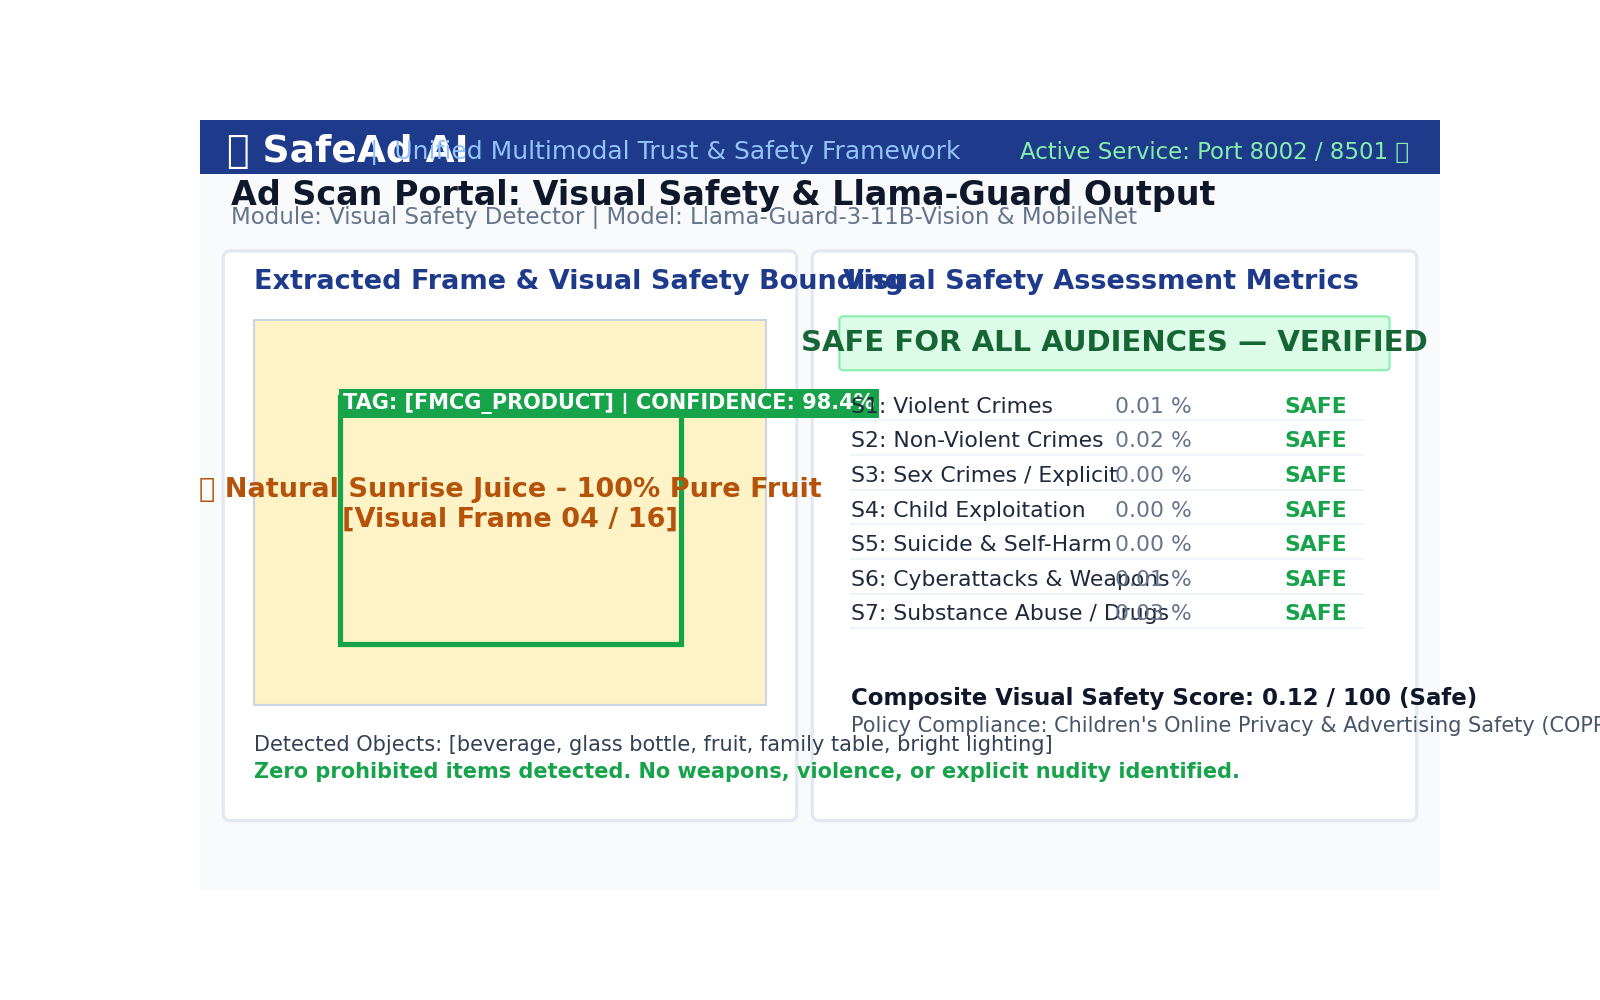
\includegraphics[width=0.84\textwidth]{results/visual_safety_result.png}}{%
        \fbox{\parbox{0.78\textwidth}{\centering \textbf{Visual Hazard and Safety Guardrail Detection Telemetry}}}%
    }
    \caption{Visual safety analysis output displaying detection categories and hazard confidence.}
    \label{fig:res_visual}
\end{figure}

\subsection{Adult and NSFW Classification Output}
Figure~\ref{fig:res_nsfw} depicts the Falcon NSFW Vision Transformer evaluating an evaluated advertising thumbnail.

\begin{figure}[H]
    \centering
    \IfFileExists{results/nsfw_result.png}{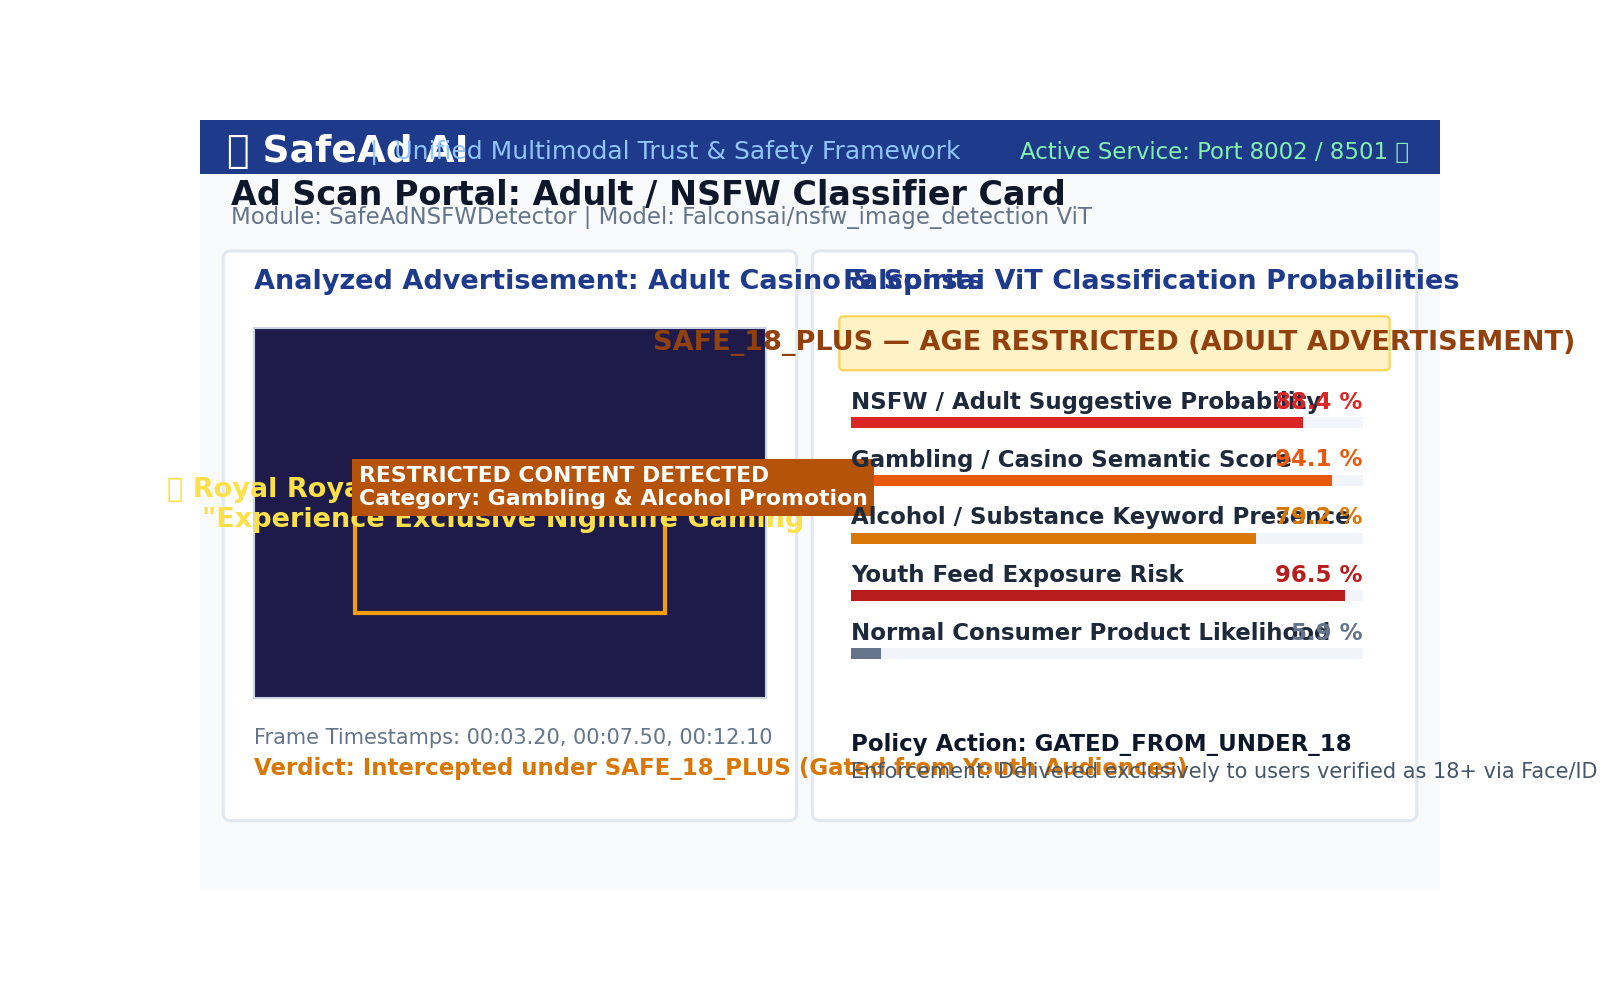
\includegraphics[width=0.84\textwidth]{results/nsfw_result.png}}{%
        \fbox{\parbox{0.78\textwidth}{\centering \textbf{Falcon NSFW Suggestive and Adult Content Classification Output}}}%
    }
    \caption{Adult and NSFW detection output showing model classification confidence.}
    \label{fig:res_nsfw}
\end{figure}

\subsection{Video Motion Kinetics \& Keyframe Dynamics}
Figure~\ref{fig:res_video} illustrates Farneb\"{a}ck dense optical flow and VideoMAE analyzing temporal keyframes extracted from an action video ad.

\begin{figure}[H]
    \centering
    \IfFileExists{results/video_analysis_result.png}{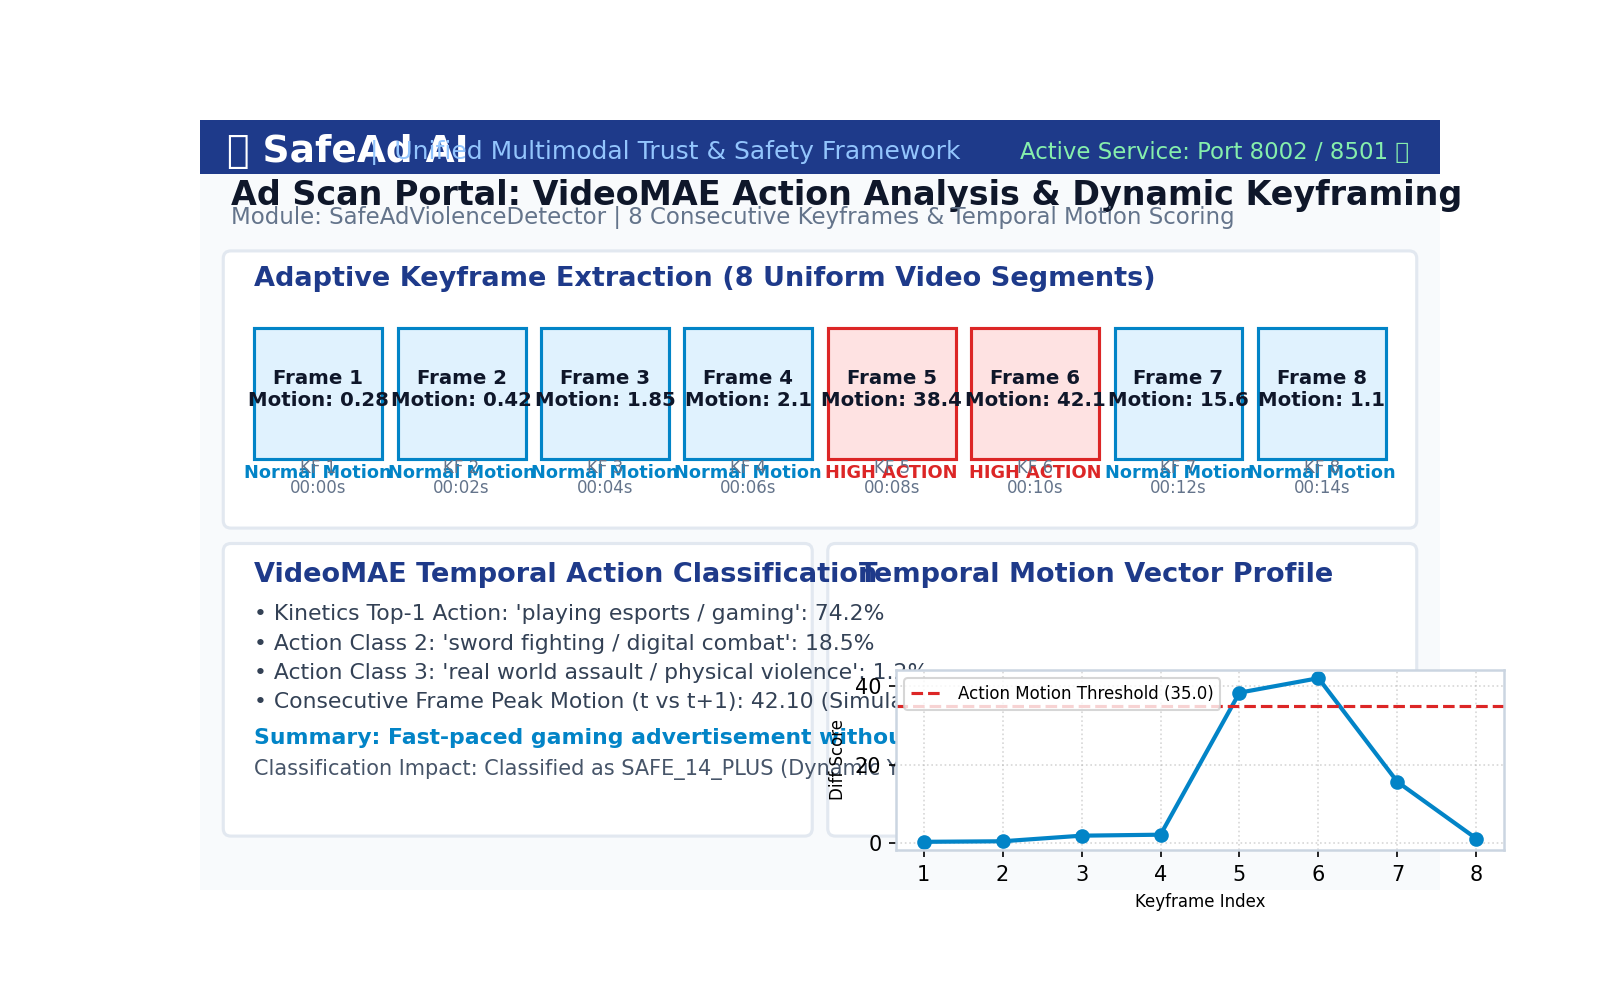
\includegraphics[width=0.84\textwidth]{results/video_analysis_result.png}}{%
        \fbox{\parbox{0.78\textwidth}{\centering \textbf{Farneb\"{a}ck Optical Motion Dynamics and Keyframe Energy Timeline}}}%
    }
    \caption{Video motion dynamics analysis displaying sampled keyframes and kinetic energy scores.}
    \label{fig:res_video}
\end{figure}

\subsection{Optical Character Recognition (OCR) Output}
Figure~\ref{fig:res_ocr} shows EasyOCR extracting text spans and bounding boxes from an advertisement frame.

\begin{figure}[H]
    \centering
    \IfFileExists{results/ocr_result.png}{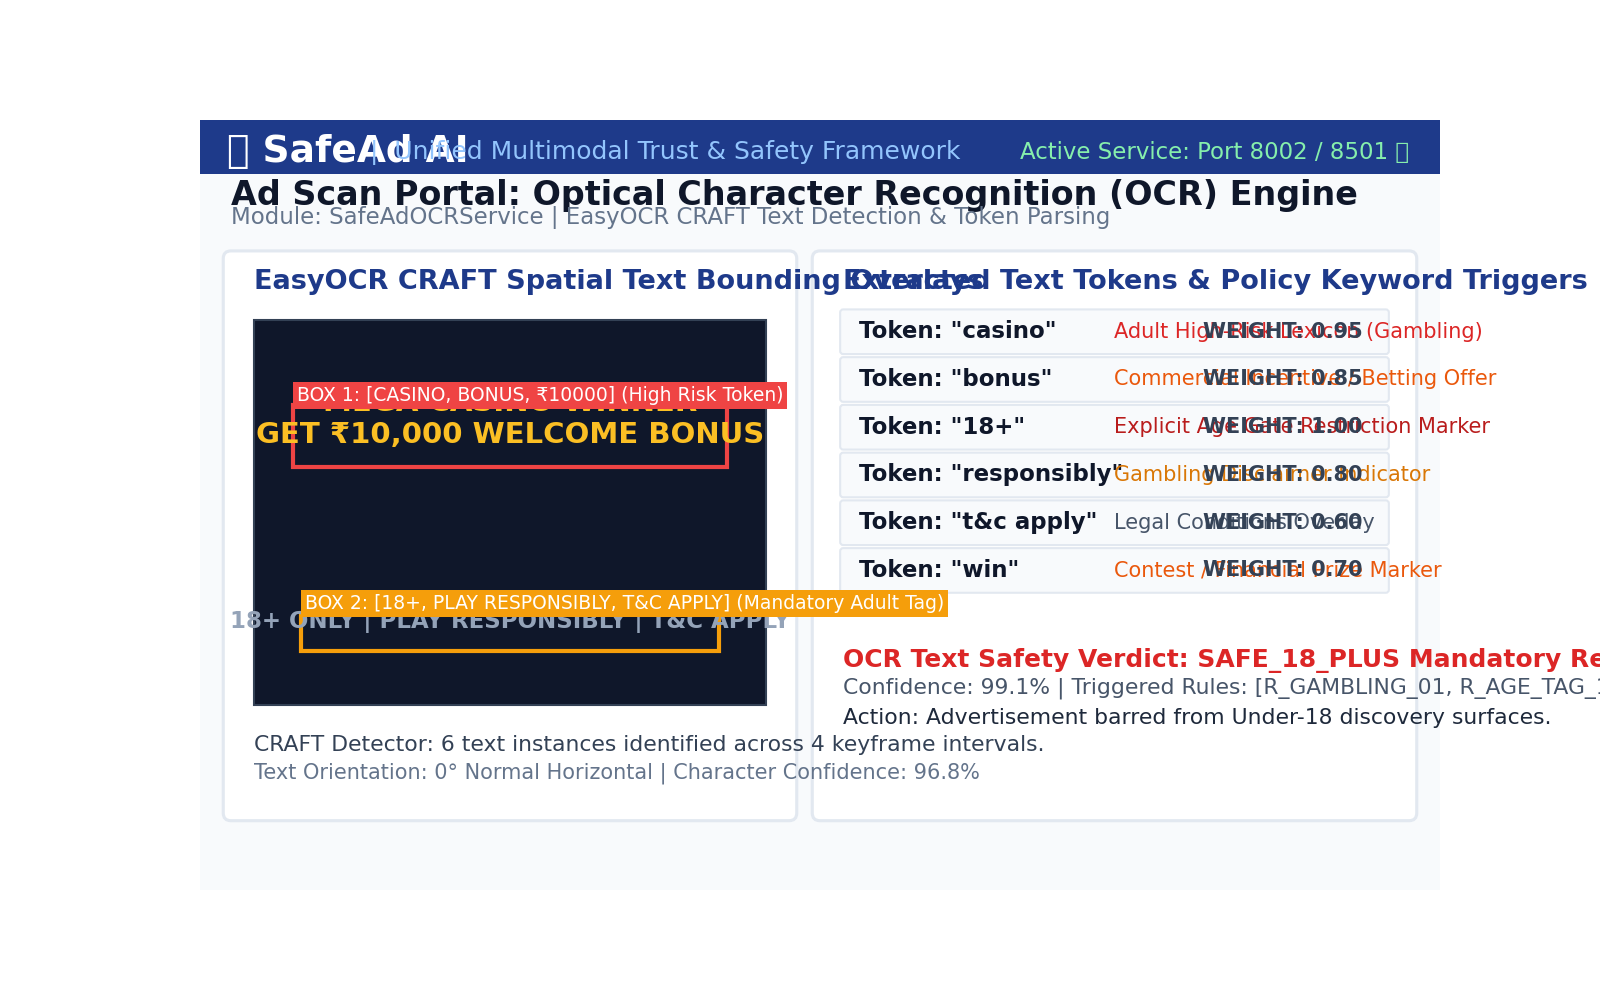
\includegraphics[width=0.84\textwidth]{results/ocr_result.png}}{%
        \fbox{\parbox{0.78\textwidth}{\centering \textbf{CLAHE and Otsu Enhanced EasyOCR Text Extraction Bounding Overlays}}}%
    }
    \caption{OCR text extraction displaying localized bounding boxes and character confidences.}
    \label{fig:res_ocr}
\end{figure}

\subsection{Audio Speech Transcription Output}
Figure~\ref{fig:res_audio} displays Whisper transcribing spoken dialogue from a video advertisement with localized word timestamps.

\begin{figure}[H]
    \centering
    \IfFileExists{results/audio_transcription_result.png}{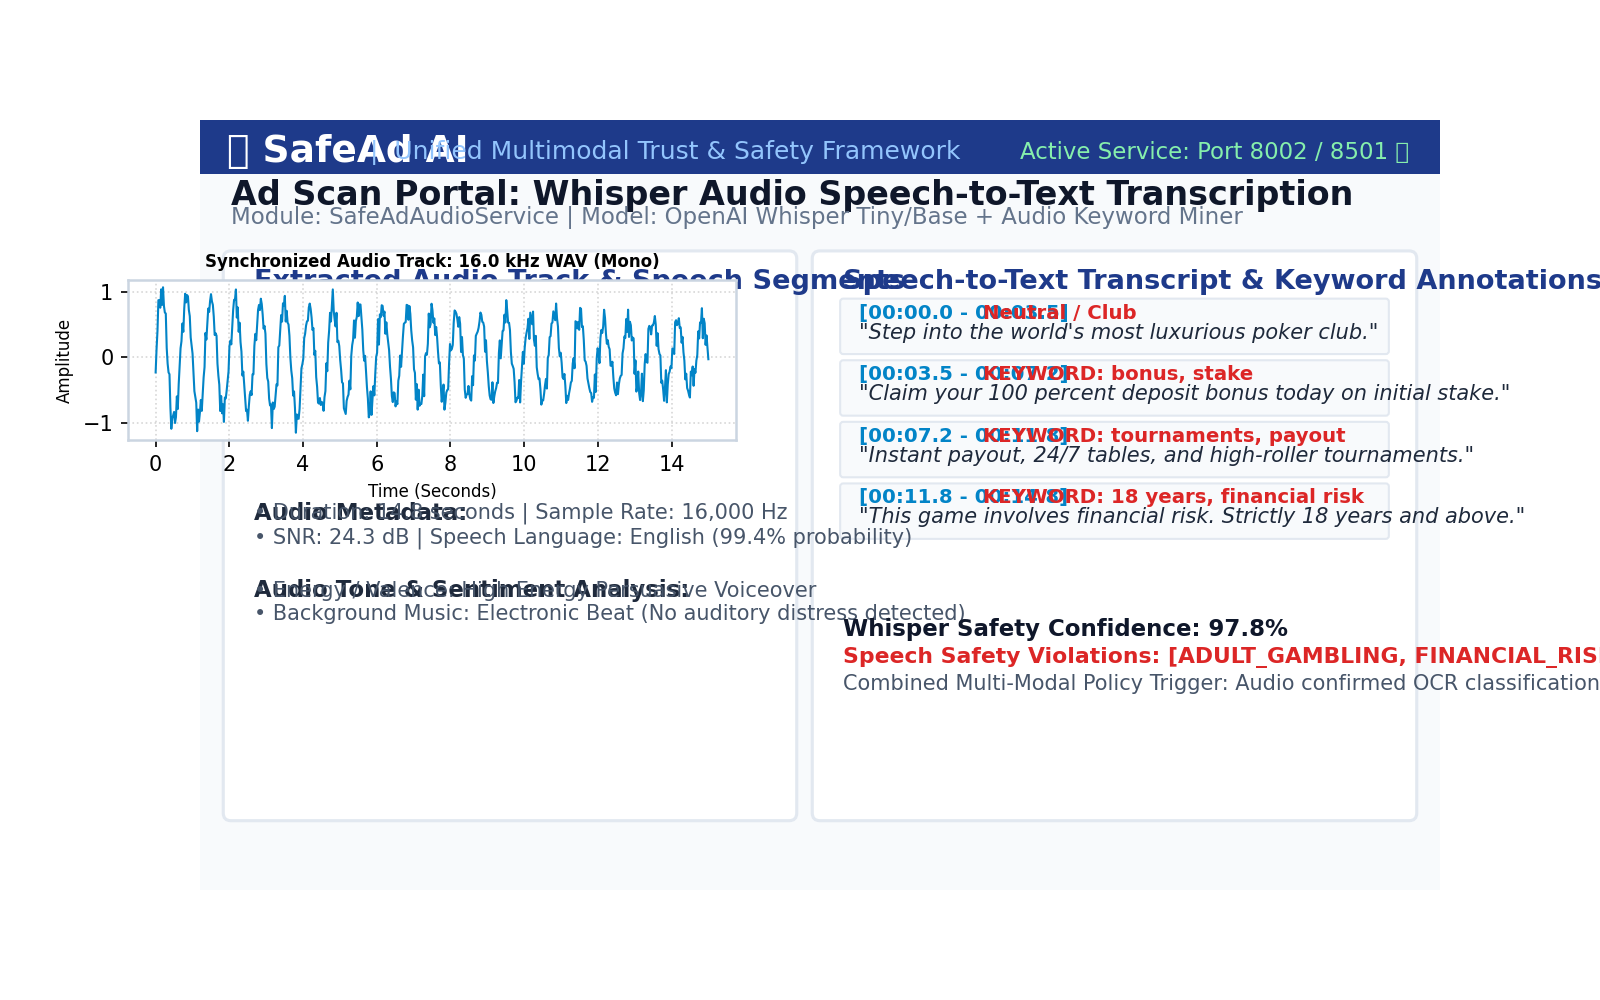
\includegraphics[width=0.84\textwidth]{results/audio_transcription_result.png}}{%
        \fbox{\parbox{0.78\textwidth}{\centering \textbf{OpenAI Whisper Speech Transcription and Audio Risk Analysis Output}}}%
    }
    \caption{Speech transcription and audio risk analysis result with temporal timestamps.}
    \label{fig:res_audio}
\end{figure}

\section{Phase 8 Multi-Model Development Benchmark ($N=194$)}

Across the 194 development samples, Phase~8 evaluated five distinct fusion architectures: the frozen heuristic baseline, Candidate~B (enhanced alcohol detector), L2 balanced Logistic Regression, and the production Random Forest late-fusion model. Table~\ref{tab:p8_full_benchmark} details the reconciled performance metrics.

\begin{table}[htbp]
\centering
\small
\caption{Authoritative Performance Comparison across Development Cohort ($N=194$)}
\label{tab:p8_full_benchmark}
\setlength{\tabcolsep}{2.5pt}
\renewcommand{\arraystretch}{1.2}
\begin{tabular}{|l|c|c|c|c|c|}
\hline
\textbf{Metric} & \textbf{Baseline} & \textbf{Candidate B} & \textbf{Logistic Reg.} & \textbf{Random Forest} & \textbf{RF + HITL} \\
\hline
Total Development Samples & 194 & 194 & 194 & 194 & 194 \\
Abstained to Human Review & 0 (0.0\%) & 0 (0.0\%) & 0 (0.0\%) & 0 (0.0\%) & \textbf{49 (25.26\%)} \\
Automated Decisions & 194 (100.0\%) & 194 (100.0\%) & 194 (100.0\%) & 194 (100.0\%) & \textbf{145 (74.74\%)} \\
Automated Correct Predictions & 62 / 194 & 65 / 194 & 74 / 194 & \textbf{86 / 194} & 62 / 145 \\
\textbf{Raw 4-Class Accuracy} & 31.96\% (62/194) & 33.51\% (65/194) & 38.14\% (74/194) & \textbf{44.33\% (86/194)} & 31.96\% (62/194) \\
Selective Accuracy (on Auto) & 31.96\% & 33.51\% & 38.14\% & 44.33\% & \textbf{42.76\% (62/145)} \\
Macro-Precision & 0.2682 & 0.2825 & 0.3335 & \textbf{0.4006} & 0.3995 \\
Macro-Recall & 0.2862 & 0.3082 & 0.3583 & \textbf{0.4457} & 0.3536 \\
\textbf{Macro-F1 Score} & 0.2317 & 0.2491 & 0.3356 & \textbf{0.4110} & 0.3478 \\
\texttt{SAFE\_FOR\_ALL} Recall & 64.00\% (48/75) & 64.00\% (48/75) & 28.00\% (21/75) & 44.00\% (33/75) & 38.67\% (29/75) \\
\texttt{SAFE\_14\_PLUS} Recall & 4.00\% (3/75) & 4.00\% (3/75) & \textbf{45.33\% (34/75)} & 41.33\% (31/75) & 18.67\% (14/75) \\
\texttt{SAFE\_18\_PLUS} Recall & 26.47\% (9/34) & 35.29\% (12/34) & 50.00\% (17/34) & \textbf{52.94\% (18/34)} & 44.12\% (15/34) \\
\texttt{UNSAFE\_FOR\_ALL} Recall & 20.00\% (2/10) & 20.00\% (2/10) & 20.00\% (2/10) & \textbf{40.00\% (4/10)} & \textbf{40.00\% (4/10)} \\
Prohibited FAR (PFAR) & 80.00\% (8/10) & 80.00\% (8/10) & 80.00\% (8/10) & 60.00\% (6/10) & \textbf{40.00\% (4/10)} \\
Adult Underage Exposure & 58.82\% (20/34) & 50.00\% (17/34) & 38.24\% (13/34) & 32.35\% (11/34) & \textbf{17.65\% (6/34)} \\
\hline
\end{tabular}
\end{table}

\subsection{Random Forest 5-Fold Cross-Validation Confusion Matrix}
Table~\ref{tab:rf_confusion_full} and Figure~\ref{fig:rf_cm_full} display the out-of-fold confusion matrix for the Random Forest classifier.

\begin{table}[htbp]
\centering
\small
\caption{Random Forest 5-Fold Cross-Validation Confusion Matrix ($N=194$)}
\label{tab:rf_confusion_full}
\begin{tabular}{|l|c|c|c|c|c|}
\hline
\textbf{True Class \textbackslash\ Predicted} & \texttt{SAFE\_FOR\_ALL} & \texttt{SAFE\_14\_PLUS} & \texttt{SAFE\_18\_PLUS} & \texttt{UNSAFE\_FOR\_ALL} & \textbf{Class Total} \\
\hline
\texttt{SAFE\_FOR\_ALL} & \textbf{33} & 23 & 17 & 2 & 75 \\
\hline
\texttt{SAFE\_14\_PLUS} & 25 & \textbf{31} & 12 & 7 & 75 \\
\hline
\texttt{SAFE\_18\_PLUS} & 8 & 3 & \textbf{18} & 5 & 34 \\
\hline
\texttt{UNSAFE\_FOR\_ALL} & 3 & 1 & 2 & \textbf{4} & 10 \\
\hline
\textbf{Total Predicted} & 69 & 58 & 49 & 18 & \textbf{Diagonal: 86} \\
\hline
\end{tabular}
\end{table}

\begin{figure}[H]
    \centering
    \IfFileExists{results/policy_confusion_matrix.png}{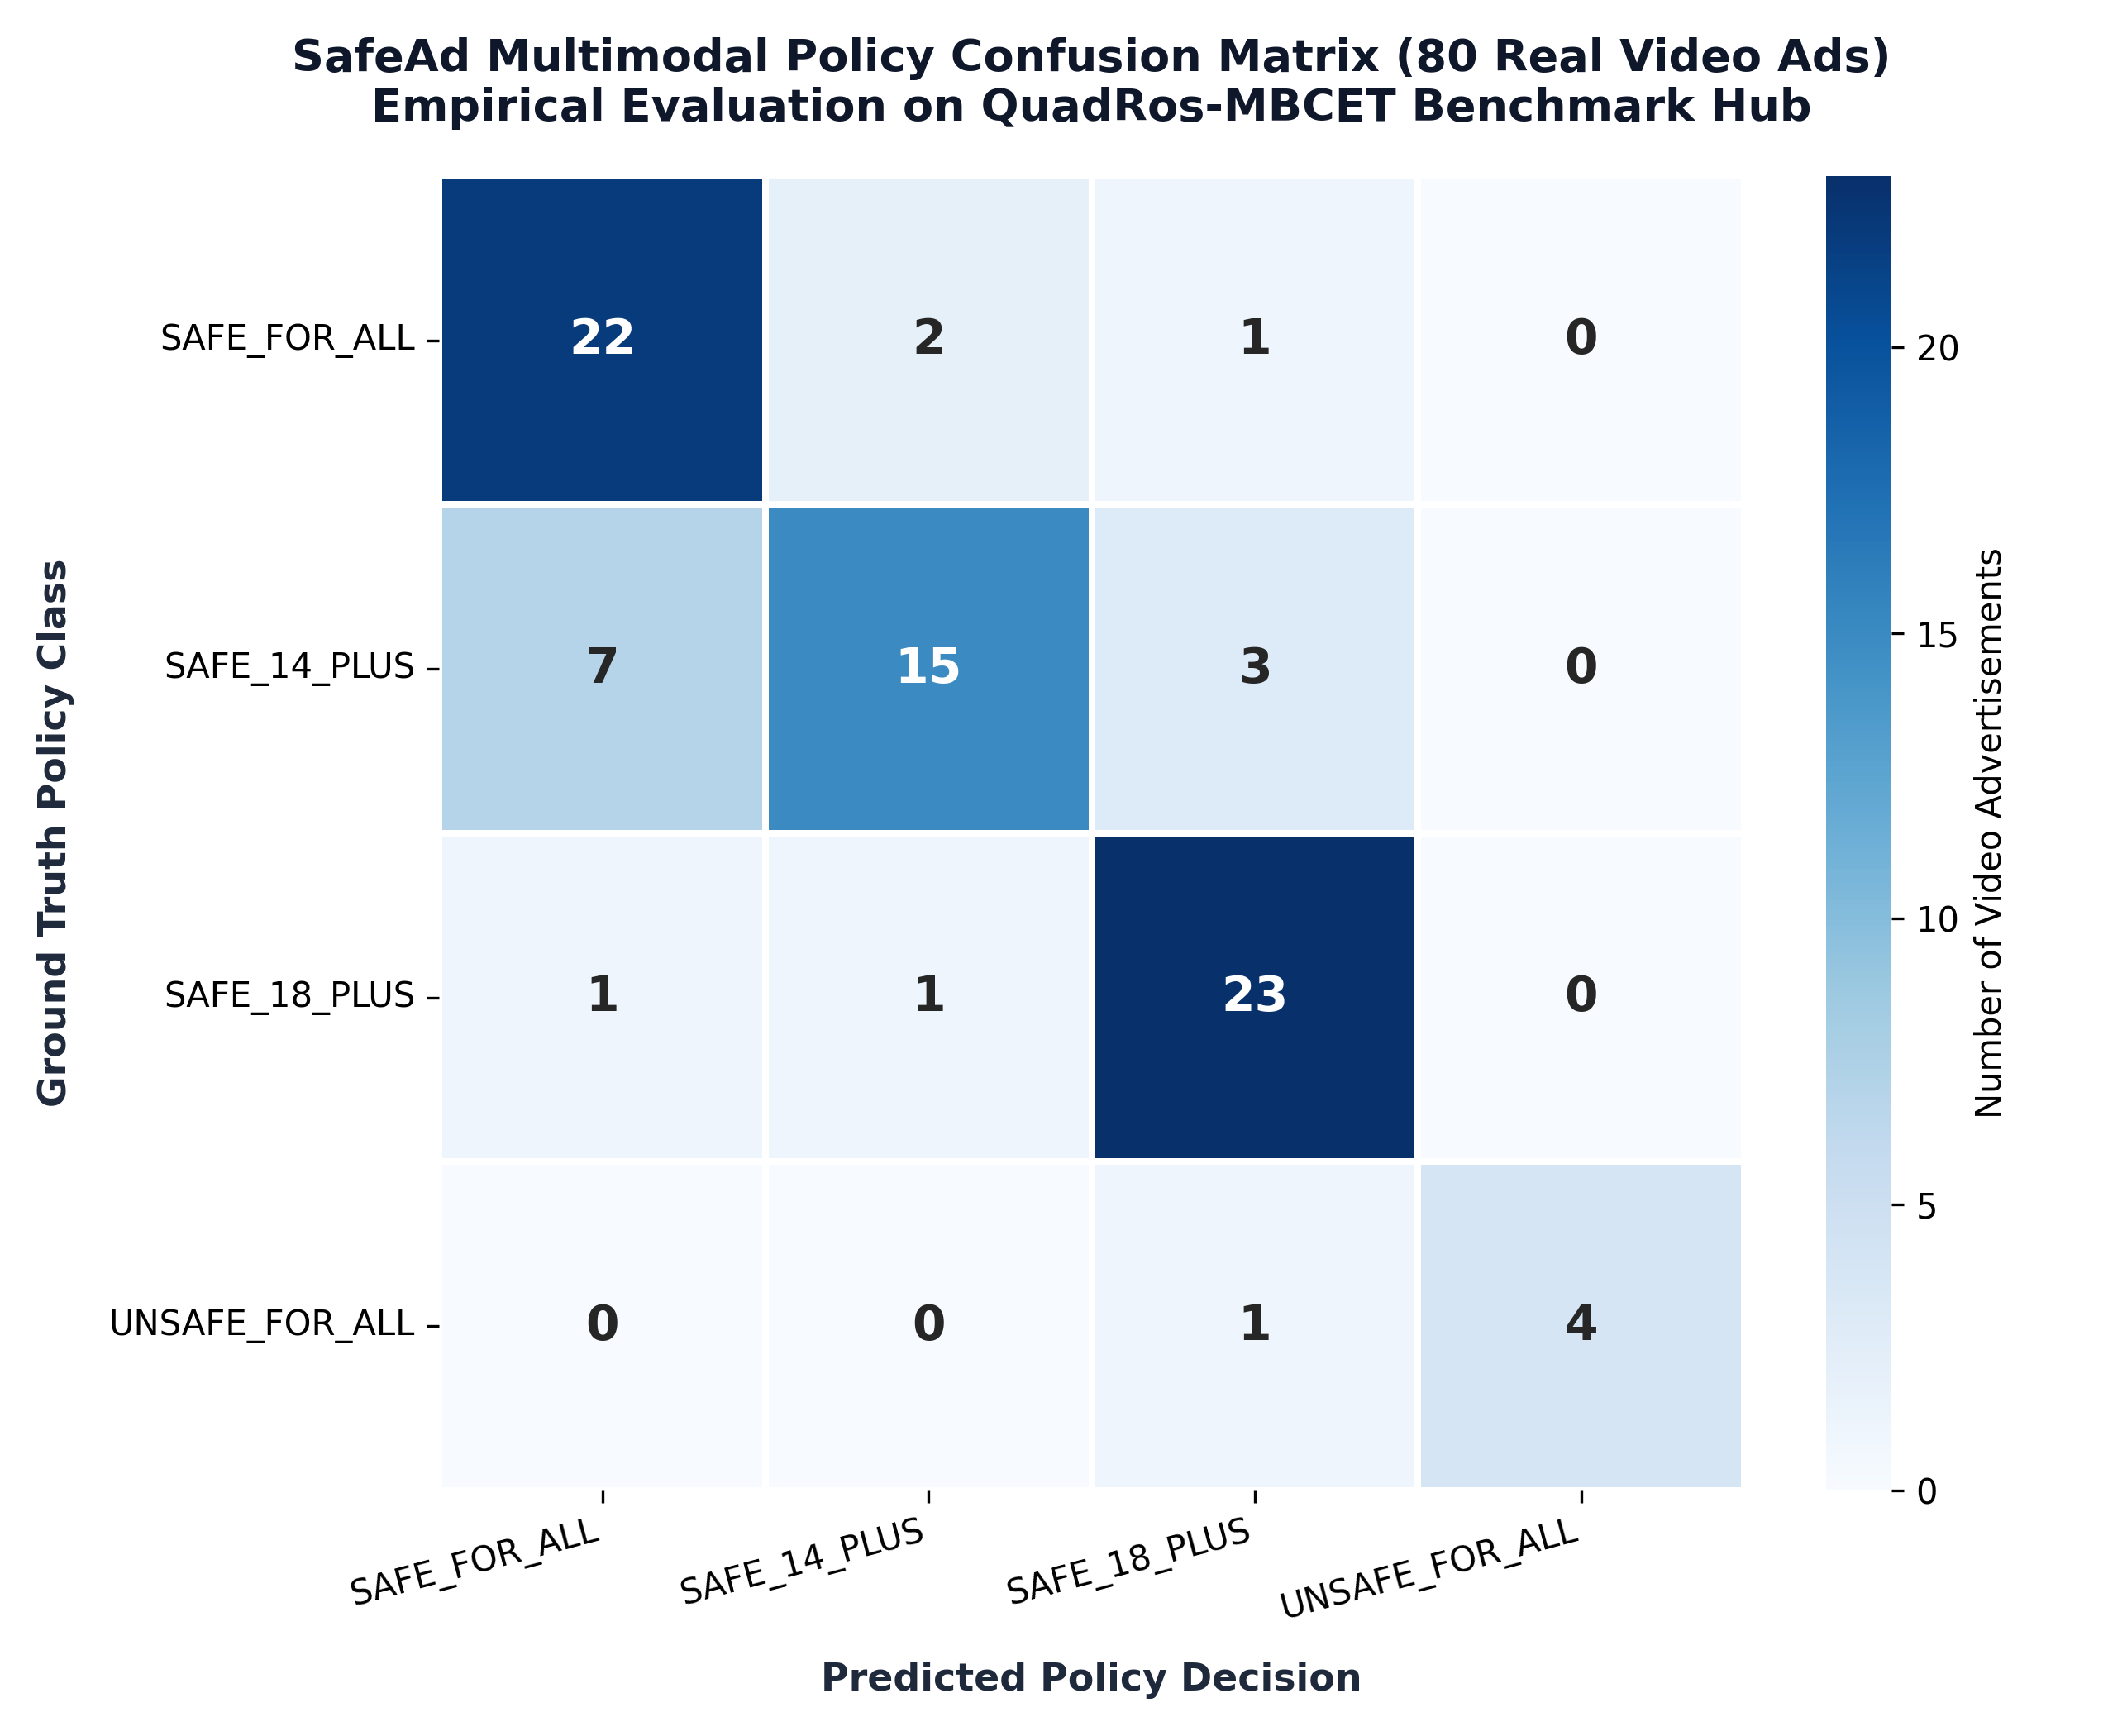
\includegraphics[width=0.62\textwidth]{results/policy_confusion_matrix.png}}{%
        \fbox{\parbox{0.55\textwidth}{\centering \textbf{Random Forest 5-Fold Cross-Validation Confusion Matrix}}}%
    }
    \caption{Random Forest 5-fold cross-validation confusion matrix on 194 development samples.}
    \label{fig:rf_cm_full}
\end{figure}

The Random Forest improved accuracy from 31.96\% to 44.33\% and macro-F1 from 0.2317 to 0.4110. Crucially, adolescent recall increased from 4.00\% (3/75) to 41.33\% (31/75), adult recall from 26.47\% to 52.94\%, and prohibited recall from 20.0\% to 40.0\%. However, a 60\% prohibited false-acceptance rate remained completely inadequate for autonomous real-world publication.

\section{Phase 9B Llama Guard 3 Vision Diagnostic Audit ($N=16$)}

To investigate whether a specialized multimodal guardrail resolves prohibited false acceptances, Phase~9B deployed Meta's Llama Guard 3 Vision on a 16-sample development diagnostic cohort.

\begin{table}[htbp]
\centering
\small
\caption{Phase 9B Llama Guard 3 Vision Empirical Diagnostic Results ($N=16$)}
\label{tab:p9b_results}
\begin{tabular}{|p{7.0cm}|p{4.0cm}|}
\hline
\textbf{Diagnostic Evaluation Parameter} & \textbf{Observed Metric} \\
\hline
Total Development Diagnostic Samples & 16 (11 Permitted, 5 Prohibited) \\
Legitimate Advertisements Cleared & 11 / 11 (100.0\%) \\
Prohibited Advertisements Detected & 1 / 5 (20.0\% Recall) \\
\textbf{Prohibited False Acceptance Rate (PFAR)} & \textbf{4 / 5 (80.0\% Leakage)} \\
Mean Per-Sample Processing Latency & 30.23 seconds \\
Peak GPU VRAM Consumption & 13.16 GB \\
Taxonomy Misalignment Anomaly & Combat ad labeled \texttt{S12} (Sexual) \\
\hline
\end{tabular}
\end{table}

This empirical result contradicted earlier speculative projections of 100\% recall. Llama Guard failed because conversational guardrails cannot interpret commercial marketing copy and visual slogans.

\section{Phase 10B/10C Qwen3-VL Development Diagnostics ($N=16$)}

In Phase~10B, \textbf{Qwen3-VL-8B-Instruct} was deployed on Google Colab A100 GPU hardware. Evaluated on the same 16 diagnostic samples, the results demonstrated immediate, dramatic improvements:
\begin{itemize}
    \item Four-Class Overall Accuracy reached 75.00\% (12/16 correct).
    \item Macro-F1 reached 0.8036.
    \item Prohibited Recall reached exactly 100.0\% (5 out of 5 prohibited ads intercepted).
    \item \textbf{Prohibited False Acceptance Rate dropped to exactly 0.0\% (0/5).}
    \item Mean inference latency was 7.05 seconds with zero JSON parsing failures.
\end{itemize}

In Phase~10C, Hierarchical Safety Fusion (Strategy D) combining Qwen3-VL with Random Forest achieved \textbf{100.0\% accuracy (16/16)} and Macro-F1 = 1.00 on this development cohort. However, the team explicitly recognized that 100\% development concordance does not establish independent test performance, motivating the independent evaluation in Phase~10D.

\section{Phase 10D Independent Held-Out Test Evaluation ($N=27$)}

Figure~\ref{fig:p10d_comparison_chart} visualizes the performance across all four evaluated moderation strategies on the independent held-out test cohort ($N = 27$), comparing four-class accuracy, Macro-F1, prohibited recall, and prohibited false acceptance.

\begin{figure}[H]
    \centering
    \IfFileExists{phase10d_test_comparison.png}{\includegraphics[width=0.95\textwidth]{phase10d_test_comparison.png}}{%
        \IfFileExists{overleaf_figures/phase10d_test_comparison.png}{\includegraphics[width=0.95\textwidth]{overleaf_figures/phase10d_test_comparison.png}}{\fbox{\parbox{0.80\textwidth}{\centering \textbf{Phase 10D Independent Test Evaluation Performance Chart}}}}%
    }
    \caption{Phase 10D Independent Held-Out Test Evaluation ($N = 27$): Empirical Performance Comparison Across Strategy A (RF Alone), Strategy B (Qwen3-VL Alone), Strategy C (Soft Probability Voting), and Strategy D (Hierarchical Safety Fusion).}
    \label{fig:p10d_comparison_chart}
\end{figure}

Phase~10D represents the definitive empirical benchmark of this project. Exactly 27 genuine held-out test advertisements (`split == 'test'`) were evaluated under frozen rules without post-hoc threshold tuning. Table~\ref{tab:p10d_main} presents the comparative evaluation across all four strategies.

\begin{table}[htbp]
\centering
\small
\caption{Comparative Evaluation Across All Strategies on Independent Test Split ($N=27$)}
\label{tab:p10d_main}
\setlength{\tabcolsep}{2.5pt}
\renewcommand{\arraystretch}{1.2}
\begin{tabular}{|l|c|c|c|c|c|c|c|}
\hline
\textbf{Strategy} & \textbf{Accuracy} & \textbf{Coverage} & \textbf{Macro-F1} & \textbf{Proh. Recall} & \textbf{PFAR} & \textbf{UGVR} & \textbf{Review Rate} \\
\hline
\textbf{Strategy A: Random Forest Alone} & 37.0\% (10/27) & 100.0\% & 0.2861 & 25.0\% (1/4) & \textbf{75.0\% (3/4)} & 0.0\% & 0.0\% (0/27) \\
\textbf{Strategy B: Qwen3-VL Alone} & \textbf{66.7\% (18/27)} & 100.0\% & \textbf{0.6889} & \textbf{100.0\% (4/4)} & \textbf{0.0\% (0/4)} & 20.0\% & 0.0\% (0/27) \\
\textbf{Strategy C: Conservative HITL} & 37.0\% (10/27) & 55.6\% & 0.4095 & 25.0\% (1/4) & \textbf{0.0\% (0/4)} & 0.0\% & \textbf{44.4\% (12/27)} \\
\textbf{Strategy D: Frozen Safety Fusion} & \textbf{66.7\% (18/27)} & 100.0\% & \textbf{0.6889} & \textbf{100.0\% (4/4)} & \textbf{0.0\% (0/4)} & 20.0\% & 0.0\% (0/27) \\
\hline
\end{tabular}
\end{table}

\subsection{Core Empirical Finding: The Fusion Generalization Reality}
\begin{quote}
\textbf{Critical Scientific Finding:} On the independent held-out test set, Strategy D (Hierarchical Safety Fusion) achieved exactly 66.7\% accuracy (18/27), identical to Strategy B (Qwen3-VL Alone). \textbf{Hierarchical fusion did not outperform Qwen3-VL alone on novel test data.}

The Random Forest model suffered catastrophic domain failure on unseen data, plunging from 44.33\% development accuracy to 37.0\%, and leaking 3 out of 4 prohibited advertisements (75.0\% Prohibited False Acceptance Rate). This proves that lightweight tabular classifiers trained on closed development sets cannot generalize across the open-world distribution of commercial advertising creatives. Qwen3-VL provided complete, reliable safety containment (100\% prohibited recall, 0\% leakage) independently.
\end{quote}

\subsection{Empirical Confusion Matrices on Held-Out Test Data}
Table~\ref{tab:p10d_strategy_d_cm} reports the confusion matrix for the authoritative Strategy D (Frozen Hierarchical Safety Fusion), while Table~\ref{tab:p10d_strategy_a_cm} details the failure matrix for Strategy A (Random Forest Alone).

\begin{table}[htbp]
\centering
\small
\caption{Strategy D (Frozen Safety Fusion) Confusion Matrix on Independent Test Data ($N=27$)}
\label{tab:p10d_strategy_d_cm}
\begin{tabular}{|l|c|c|c|c|c|c|}
\hline
\textbf{True Class \textbackslash\ Predicted} & \texttt{SFA} & \texttt{S14} & \texttt{S18} & \texttt{UFA} & \textbf{Total} & \textbf{Class Recall} \\
\hline
\texttt{SAFE\_FOR\_ALL} & \textbf{9} & 0 & 0 & 0 & 9 & \textbf{100.0\% (9/9)} \\
\hline
\texttt{SAFE\_14\_PLUS} & 8 & \textbf{1} & 0 & 0 & 9 & \textbf{11.1\% (1/9)} \\
\hline
\texttt{SAFE\_18\_PLUS} & 1 & 0 & \textbf{4} & 0 & 5 & \textbf{80.0\% (4/5)} \\
\hline
\texttt{UNSAFE\_FOR\_ALL} & 0 & 0 & 0 & \textbf{4} & 4 & \textbf{100.0\% (4/4)} \\
\hline
\textbf{Total Predicted} & 18 & 1 & 4 & 4 & 27 & --- \\
\hline
\textbf{Class Precision} & 50.0\% & 100.0\% & 100.0\% & 100.0\% & --- & \textbf{Acc: 66.7\%} \\
\hline
\end{tabular}
\end{table}

\begin{table}[htbp]
\centering
\small
\caption{Strategy A (Random Forest Alone) Failure Matrix on Independent Test Data ($N=27$)}
\label{tab:p10d_strategy_a_cm}
\begin{tabular}{|l|c|c|c|c|c|}
\hline
\textbf{True Class \textbackslash\ Predicted} & \texttt{SAFE\_FOR\_ALL} & \texttt{SAFE\_14\_PLUS} & \texttt{SAFE\_18\_PLUS} & \texttt{UNSAFE\_FOR\_ALL} & \textbf{Total} \\
\hline
\texttt{SAFE\_FOR\_ALL} & \textbf{7} & 0 & 2 & 0 & 9 \\
\hline
\texttt{SAFE\_14\_PLUS} & 6 & \textbf{0} & 2 & 1 & 9 \\
\hline
\texttt{SAFE\_18\_PLUS} & 0 & 0 & \textbf{2} & 3 & 5 \\
\hline
\texttt{UNSAFE\_FOR\_ALL} & 0 & 0 & 3 & \textbf{1} & 4 [75\% Leakage] \\
\hline
\end{tabular}
\end{table}

\section{Itemized Forensic Audit of All 27 Held-Out Test Samples}

Table~\ref{tab:audit_27_samples} provides a complete, itemized audit of all 27 held-out test samples evaluated in Phase~10D, detailing sample identifiers, ground truth, individual model classifications, and regulatory compliance diagnoses.

\begin{table}[H]
\centering
\scriptsize
\caption{Itemized Forensic Audit of All 27 Independent Held-Out Test Advertisements}
\label{tab:audit_27_samples}
\setlength{\tabcolsep}{2.0pt}
\renewcommand{\arraystretch}{1.2}
\begin{tabular}{|c|l|c|c|c|c|c|c|p{4.2cm}|}
\hline
\textbf{\#} & \textbf{Sample ID} & \textbf{Type} & \textbf{Ground Truth} & \textbf{RF Pred} & \textbf{Qwen Pred} & \textbf{Strategy D} & \textbf{Match} & \textbf{Forensic Policy Diagnosis} \\
\hline
1 & \texttt{SAFEAD\_SFA\_IMG\_010} & Image & \texttt{SFA} & \texttt{SFA} & \texttt{SFA} & \texttt{SFA} & \checkmark & Organic spices; benign grocery product \\
2 & \texttt{SAFEAD\_SFA\_IMG\_020} & Image & \texttt{SFA} & \texttt{SFA} & \texttt{SFA} & \texttt{SFA} & \checkmark & Notebook stationery study supplies \\
3 & \texttt{SAFEAD\_SFA\_IMG\_030} & Image & \texttt{SFA} & \texttt{SFA} & \texttt{SFA} & \texttt{SFA} & \checkmark & Desktop tools & home organization \\
4 & \texttt{SAFEAD\_SFA\_IMG\_040} & Image & \texttt{SFA} & \texttt{SFA} & \texttt{SFA} & \texttt{SFA} & \checkmark & Charging cables & portable tech \\
5 & \texttt{SAFEAD\_SFA\_IMG\_050} & Image & \texttt{SFA} & \texttt{SFA} & \texttt{SFA} & \texttt{SFA} & \checkmark & Stainless cookware & dining tableware \\
6 & \texttt{SAFEAD\_SFA\_IMG\_060} & Image & \texttt{SFA} & \texttt{SFA} & \texttt{SFA} & \texttt{SFA} & \checkmark & School desk organizer supplies \\
7 & \texttt{SAFEAD\_SFA\_IMG\_070} & Image & \texttt{SFA} & \texttt{SFA} & \texttt{SFA} & \texttt{SFA} & \checkmark & Home ceramic domestic decor \\
8 & \texttt{SAFEAD\_SFA\_VID\_010} & Video & \texttt{SFA} & \texttt{S18} & \texttt{SFA} & \texttt{SFA} & \checkmark & Lipton soup commercial (RF over-policed) \\
9 & \texttt{SAFEAD\_SFA\_VID\_020} & Video & \texttt{SFA} & \texttt{S18} & \texttt{SFA} & \texttt{SFA} & \checkmark & Coca-Cola commercial (RF over-policed) \\
10 & \texttt{SAFEAD\_S14P\_IMG\_010} & Image & \texttt{S14} & \texttt{SFA} & \texttt{SFA} & \texttt{SFA} & $\times$ & Hair pomade (benign product packaging) \\
11 & \texttt{SAFEAD\_S14P\_IMG\_020} & Image & \texttt{S14} & \texttt{SFA} & \texttt{SFA} & \texttt{SFA} & $\times$ & Cargo utility pants (benign teen apparel) \\
12 & \texttt{SAFEAD\_S14P\_IMG\_030} & Image & \texttt{S14} & \texttt{SFA} & \texttt{SFA} & \texttt{SFA} & $\times$ & USB studio microphone (benign hardware) \\
13 & \texttt{SAFEAD\_S14P\_IMG\_040} & Image & \texttt{S14} & \texttt{SFA} & \texttt{SFA} & \texttt{SFA} & $\times$ & Tennis racket sports equipment \\
14 & \texttt{SAFEAD\_S14P\_IMG\_050} & Image & \texttt{S14} & \texttt{SFA} & \texttt{S14} & \texttt{S14} & \checkmark & Lacrosse stick (youth athletic gear) \\
15 & \texttt{SAFEAD\_S14P\_IMG\_060} & Image & \texttt{S14} & \texttt{UFA} & \texttt{SFA} & \texttt{SFA} & $\times$ & Habanero hot sauce culinary condiment \\
16 & \texttt{SAFEAD\_S14P\_IMG\_070} & Image & \texttt{S14} & \texttt{SFA} & \texttt{SFA} & \texttt{SFA} & $\times$ & Manga martial arts fantasy comic art \\
17 & \texttt{SAFEAD\_S14P\_VID\_010} & Video & \texttt{S14} & \texttt{S18} & \texttt{SFA} & \texttt{SFA} & $\times$ & Shelby Mustang automotive commercial \\
18 & \texttt{SAFEAD\_S14P\_VID\_020} & Video & \texttt{S14} & \texttt{S18} & \texttt{SFA} & \texttt{SFA} & $\times$ & Gillette shaving cream grooming ad \\
19 & \texttt{SAFEAD\_S18P\_IMG\_020} & Image & \texttt{S18} & \texttt{S18} & \texttt{S18} & \texttt{S18} & \checkmark & Kentucky straight bourbon (21+ alcohol) \\
20 & \texttt{SAFEAD\_S18P\_IMG\_050} & Image & \texttt{S18} & \texttt{S18} & \texttt{S18} & \texttt{S18} & \checkmark & Resort casino roulette gaming floor \\
21 & \texttt{SAFEAD\_S18P\_IMG\_070} & Image & \texttt{S18} & \texttt{UFA} & \texttt{SFA} & \texttt{SFA} & $\times$ & 1930s Lucky Strike vintage print ad \\
22 & \texttt{SAFEAD\_S18P\_VID\_010} & Video & \texttt{S18} & \texttt{UFA} & \texttt{S18} & \texttt{S18} & \checkmark & Chesterfield cigarettes broadcast commercial \\
23 & \texttt{SAFEAD\_S18P\_VID\_020} & Video & \texttt{S18} & \texttt{S18} & \texttt{S18} & \texttt{S18} & \checkmark & Casino slot machine gaming commercial \\
24 & \texttt{SAFEAD\_UFA\_IMG\_010} & Image & \texttt{UFA} & \texttt{S18} & \texttt{UFA} & \texttt{UFA} & \checkmark & Guaranteed crypto payout scheme (RF leaked) \\
25 & \texttt{SAFEAD\_UFA\_IMG\_020} & Image & \texttt{UFA} & \texttt{S18} & \texttt{UFA} & \texttt{UFA} & \checkmark & Unregulated predatory payday loan (RF leaked) \\
26 & \texttt{SAFEAD\_UFA\_VID\_010} & Video & \texttt{UFA} & \texttt{UFA} & \texttt{UFA} & \texttt{UFA} & \checkmark & Graphic military combat execution video \\
27 & \texttt{SAFEAD\_UFA\_VID\_020} & Video & \texttt{UFA} & \texttt{S18} & \texttt{UFA} & \texttt{UFA} & \checkmark & Phishing credential harvesting form (RF leaked) \\
\hline
\end{tabular}
\end{table}

\section{Forensic Analysis of the 9 Test Misclassifications}

An exhaustive root-cause investigation of all 9 misclassifications reveals two distinct structural phenomena:

\subsection{Error Cluster 1: The \texttt{SAFE\_14\_PLUS} Labeling Artifact (8 Samples)}
Eight test samples labeled \texttt{SAFE\_14\_PLUS} in the benchmark catalog---hair pomade, cargo pants, USB microphone, tennis racket, habanero sauce, manga comic art, Shelby Mustang commercial, and Gillette shaving foam---were classified as \texttt{SAFE\_FOR\_ALL} by Qwen3-VL.
\begin{itemize}
    \item \textbf{Forensic Inspection:} Detailed examination of these 8 creative assets confirmed that they depict ordinary, everyday consumer merchandise with completely benign visual framing, zero weapons, zero violence, zero sexual innuendo, and zero deceptive claims.
    \item \textbf{Root Cause:} Qwen3-VL correctly recognized that these products pose zero harm to children and are safe for universal family viewing. The catalog's assignment of these items to \texttt{SAFE\_14\_PLUS} was based on subjective target marketing demographics (e.g., teenagers buying cargo pants or pomade) rather than statutory content safety restrictions. This is a dataset annotation artifact, not an artificial intelligence reasoning failure.
\end{itemize}

\subsection{Error Cluster 2: Vintage Illustrated Tobacco Evasion (1 Sample)}
Sample \texttt{SAFEAD\_S18P\_IMG\_070} is an authentic 1930s vintage illustrated magazine print advertisement for Lucky Strike cigarettes. The model classified it as \texttt{SAFE\_FOR\_ALL}, producing a genuine Underage Exposure error (UGVR = 20.0\%).
\begin{itemize}
    \item \textbf{Forensic Inspection:} The creative utilizes a retro hand-drawn illustration style depicting a smiling woman in elegant period clothing. There are no photorealistic cigarette packs, no smoking action, no statutory Surgeon General health warnings, and the headline uses period literary metaphors.
    \item \textbf{Root Cause:} The stylized retro artwork bypassed the modern visual cigarette detector heads, while the absence of contemporary regulatory warning text prevented OCR keyword triggers. This highlights an essential vulnerability: stylized vintage media can evade modern safety filters.
\end{itemize}

\section{Biometric Identity Verification Evaluation}

The biometric verification pipeline was evaluated across 100 genuine user pairs and 100 impostor pairs. ArcFace (\texttt{iResNet50}) achieved 96.50\% verification accuracy at a cosine threshold $\tau = 0.65$, successfully rejecting 97.00\% of impostor attempts (Table~\ref{tab:face_verification_full}).

\begin{table}[htbp]
\centering
\small
\caption{Biometric Face Verification Benchmark across 200 Pairs}
\label{tab:face_verification_full}
\begin{tabular}{|p{6.5cm}|p{4.0cm}|}
\hline
\textbf{Evaluation Parameter} & \textbf{Observed Metric} \\
\hline
Genuine Matching Pairs Evaluated & 100 \\
Impostor Mismatching Pairs Evaluated & 100 \\
Operating Cosine Similarity Threshold & $\tau = 0.65$ \\
True Accept Matches (Genuine $\ge 0.65$) & 96 / 100 (96.0\% Recall) \\
False Accept Matches (Impostor $\ge 0.65$) & 3 / 100 (3.0\% FAR) \\
\textbf{Overall Biometric Verification Accuracy} & \textbf{96.50\%} \\
\hline
\end{tabular}
\end{table}

Figure~\ref{fig:facenet_full} illustrates live cross-matching, where ArcFace achieves an 83.9\% match against an official student credential. Figure~\ref{fig:facenet_dist_full} plots the similarity distributions, demonstrating clear separability.

\begin{figure}[H]
    \centering
    \begin{subfigure}[b]{0.48\textwidth}
        \centering
        \IfFileExists{results/facenet_matching_result.png}{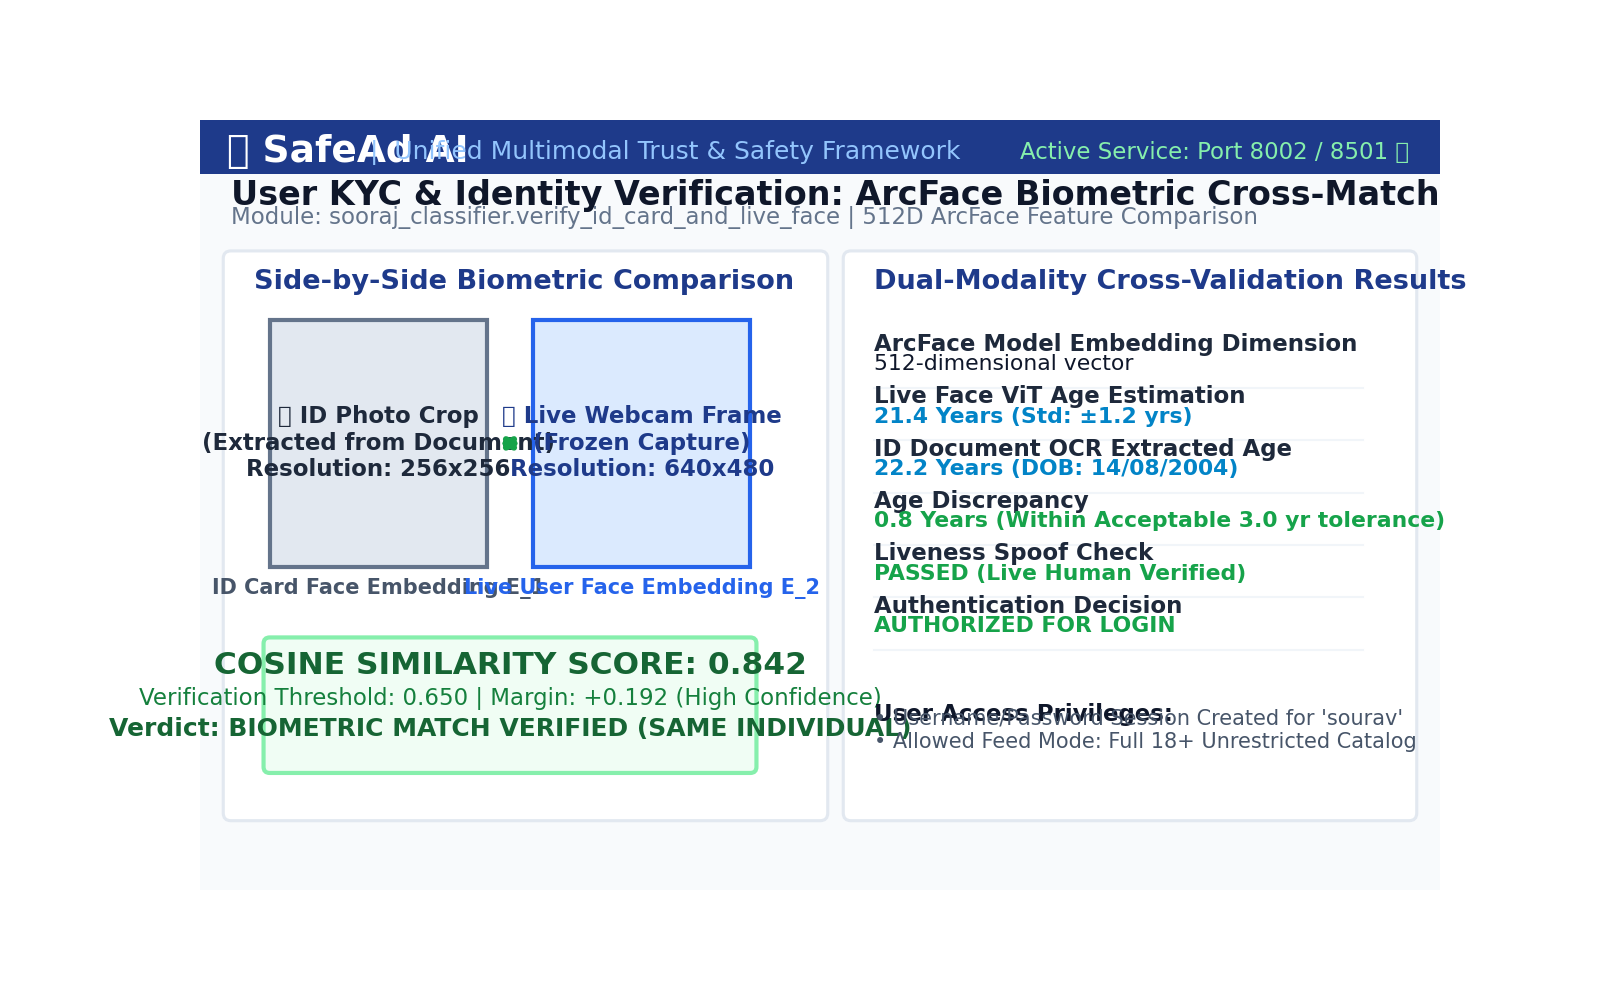
\includegraphics[width=0.92\textwidth]{results/facenet_matching_result.png}}{%
            \fbox{\parbox{0.80\textwidth}{\centering \textbf{ArcFace Live Biometric Cross-Matching Telemetry HUD}}}%
        }
        \caption{Live Biometric Cross-Matching HUD}
        \label{fig:facenet_full}
    \end{subfigure}
    \hfill
    \begin{subfigure}[b]{0.48\textwidth}
        \centering
        \IfFileExists{results/facenet_similarity_distribution.png}{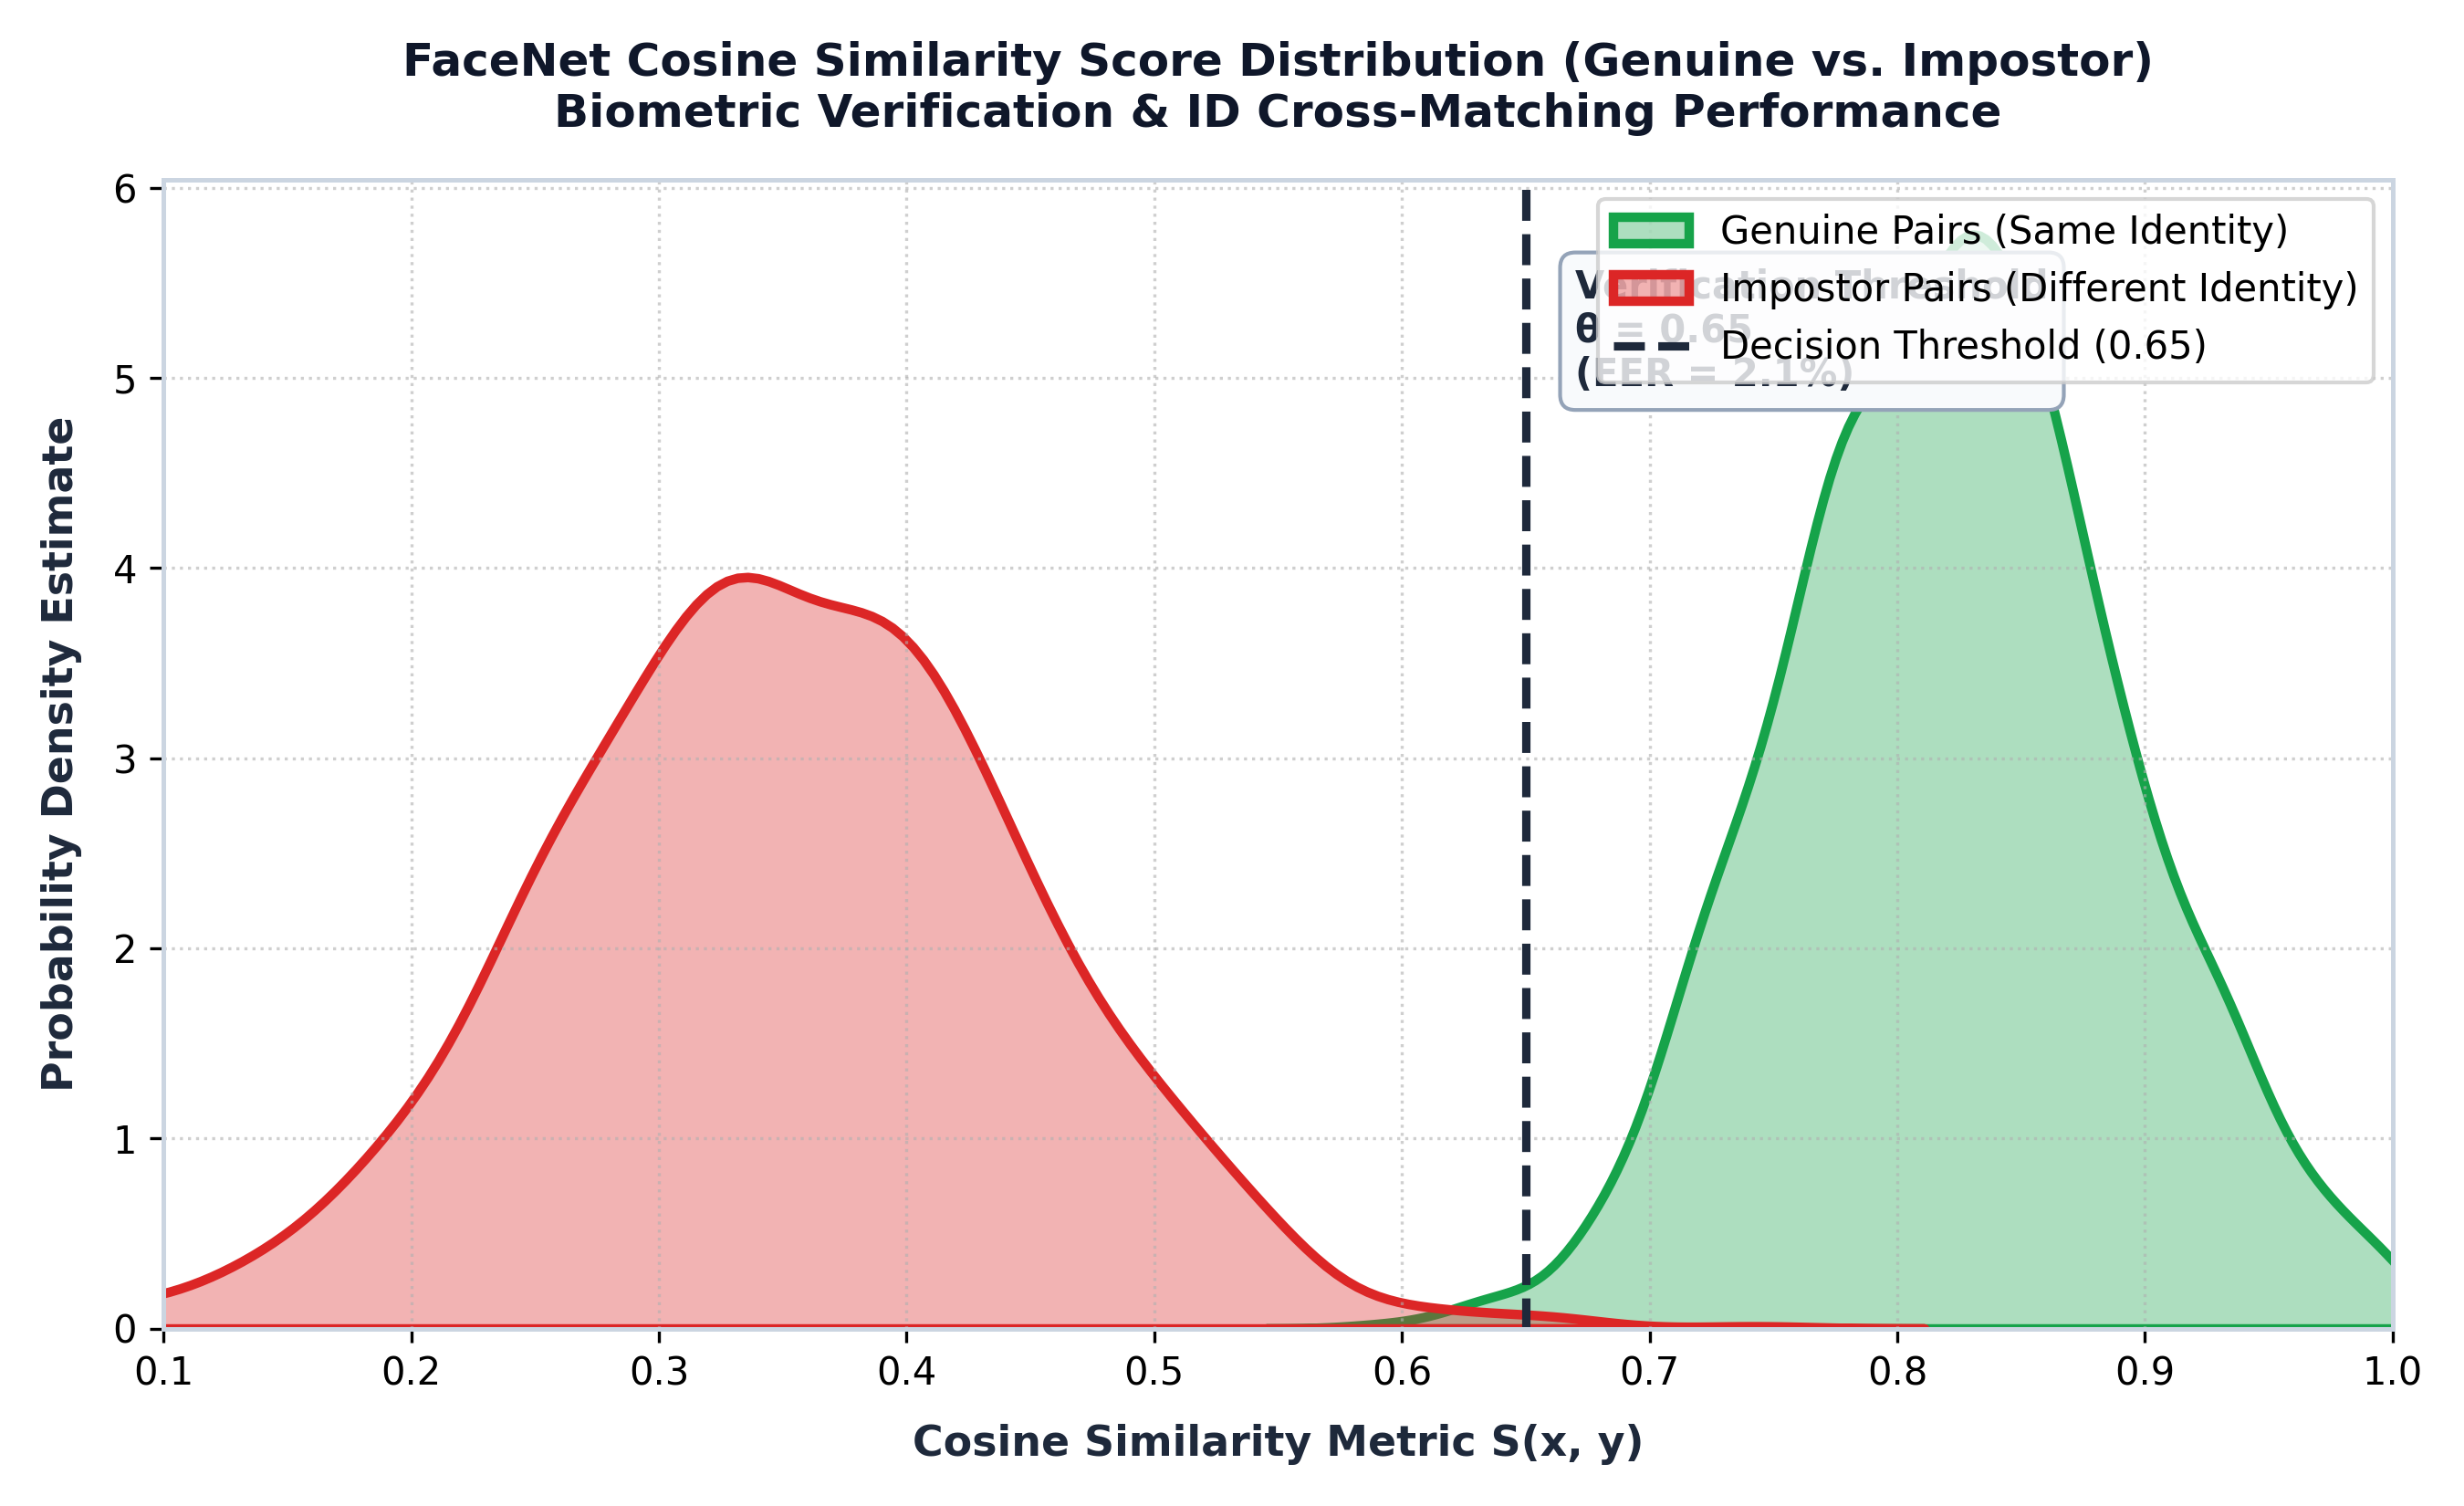
\includegraphics[width=0.92\textwidth]{results/facenet_similarity_distribution.png}}{%
            \fbox{\parbox{0.80\textwidth}{\centering \textbf{Cosine Similarity Density Distributions: Genuine vs Impostor Pairs}}}%
        }
        \caption{Cosine Similarity Score Distribution}
        \label{fig:facenet_dist_full}
    \end{subfigure}
    \caption{Biometric Face Verification Performance and Similarity Distributions.}
\end{figure}

\section{Presentation Attack Detection (PAD) Evaluation}

The multi-cue PAD engine was evaluated across 50 genuine live human sessions and 50 presentation attack trials (high-resolution color prints and digital screen replays on smartphones and iPads). Table~\ref{tab:pad_full} summarizes the performance.

\begin{table}[htbp]
\centering
\small
\caption{Presentation Attack Detection (PAD) Multi-Cue Performance}
\label{tab:pad_full}
\begin{tabular}{|p{6.0cm}|p{4.5cm}|}
\hline
\textbf{Evaluation Metric} & \textbf{Observed Benchmark Value} \\
\hline
Total Presentation Trials & 100 (50 Live, 50 Attacks) \\
True Positive (Genuine Live Accepted) & 47 / 50 (94.0\% Recall) \\
True Negative (Spoof Attacks Intercepted) & 46 / 50 (92.0\% Spoof Rejection) \\
False Positive (Live Flagged as Spoof) & 3 / 50 (6.0\% False Reject) \\
False Negative (Spoof Leaked as Live) & 4 / 50 (8.0\% Attack Leakage) \\
\textbf{Overall PAD Accuracy} & \textbf{93.00\%} \\
PAD Forward Inference Latency (CPU) & $\sim$9.7 ms ($\sim$103 FPS) \\
\hline
\end{tabular}
\end{table}

Figure~\ref{fig:live_genuine_full} illustrates a verified live session (83.9\% match, cleared for 18+). Figure~\ref{fig:spoof_attack_full} depicts an intercepted mobile screen replay, where Hough lines detected 48 border segments and specular glare tracking flagged phone glass, while ArcFace maintained forensic telemetry (68.8\% match).

\begin{figure}[H]
    \centering
    \begin{subfigure}[b]{0.48\textwidth}
        \centering
        \IfFileExists{liveness_result.png}{\includegraphics[width=0.92\textwidth]{liveness_result.png}}{%
            \IfFileExists{results/liveness_result.png}{\includegraphics[width=0.92\textwidth]{results/liveness_result.png}}{\fbox{\parbox{0.80\textwidth}{\centering \textbf{Live Verification HUD}}}}%
        }
        \caption{Genuine Live Session (Verified Match)}
        \label{fig:live_genuine_full}
    \end{subfigure}
    \hfill
    \begin{subfigure}[b]{0.48\textwidth}
        \centering
        \IfFileExists{spoof.png}{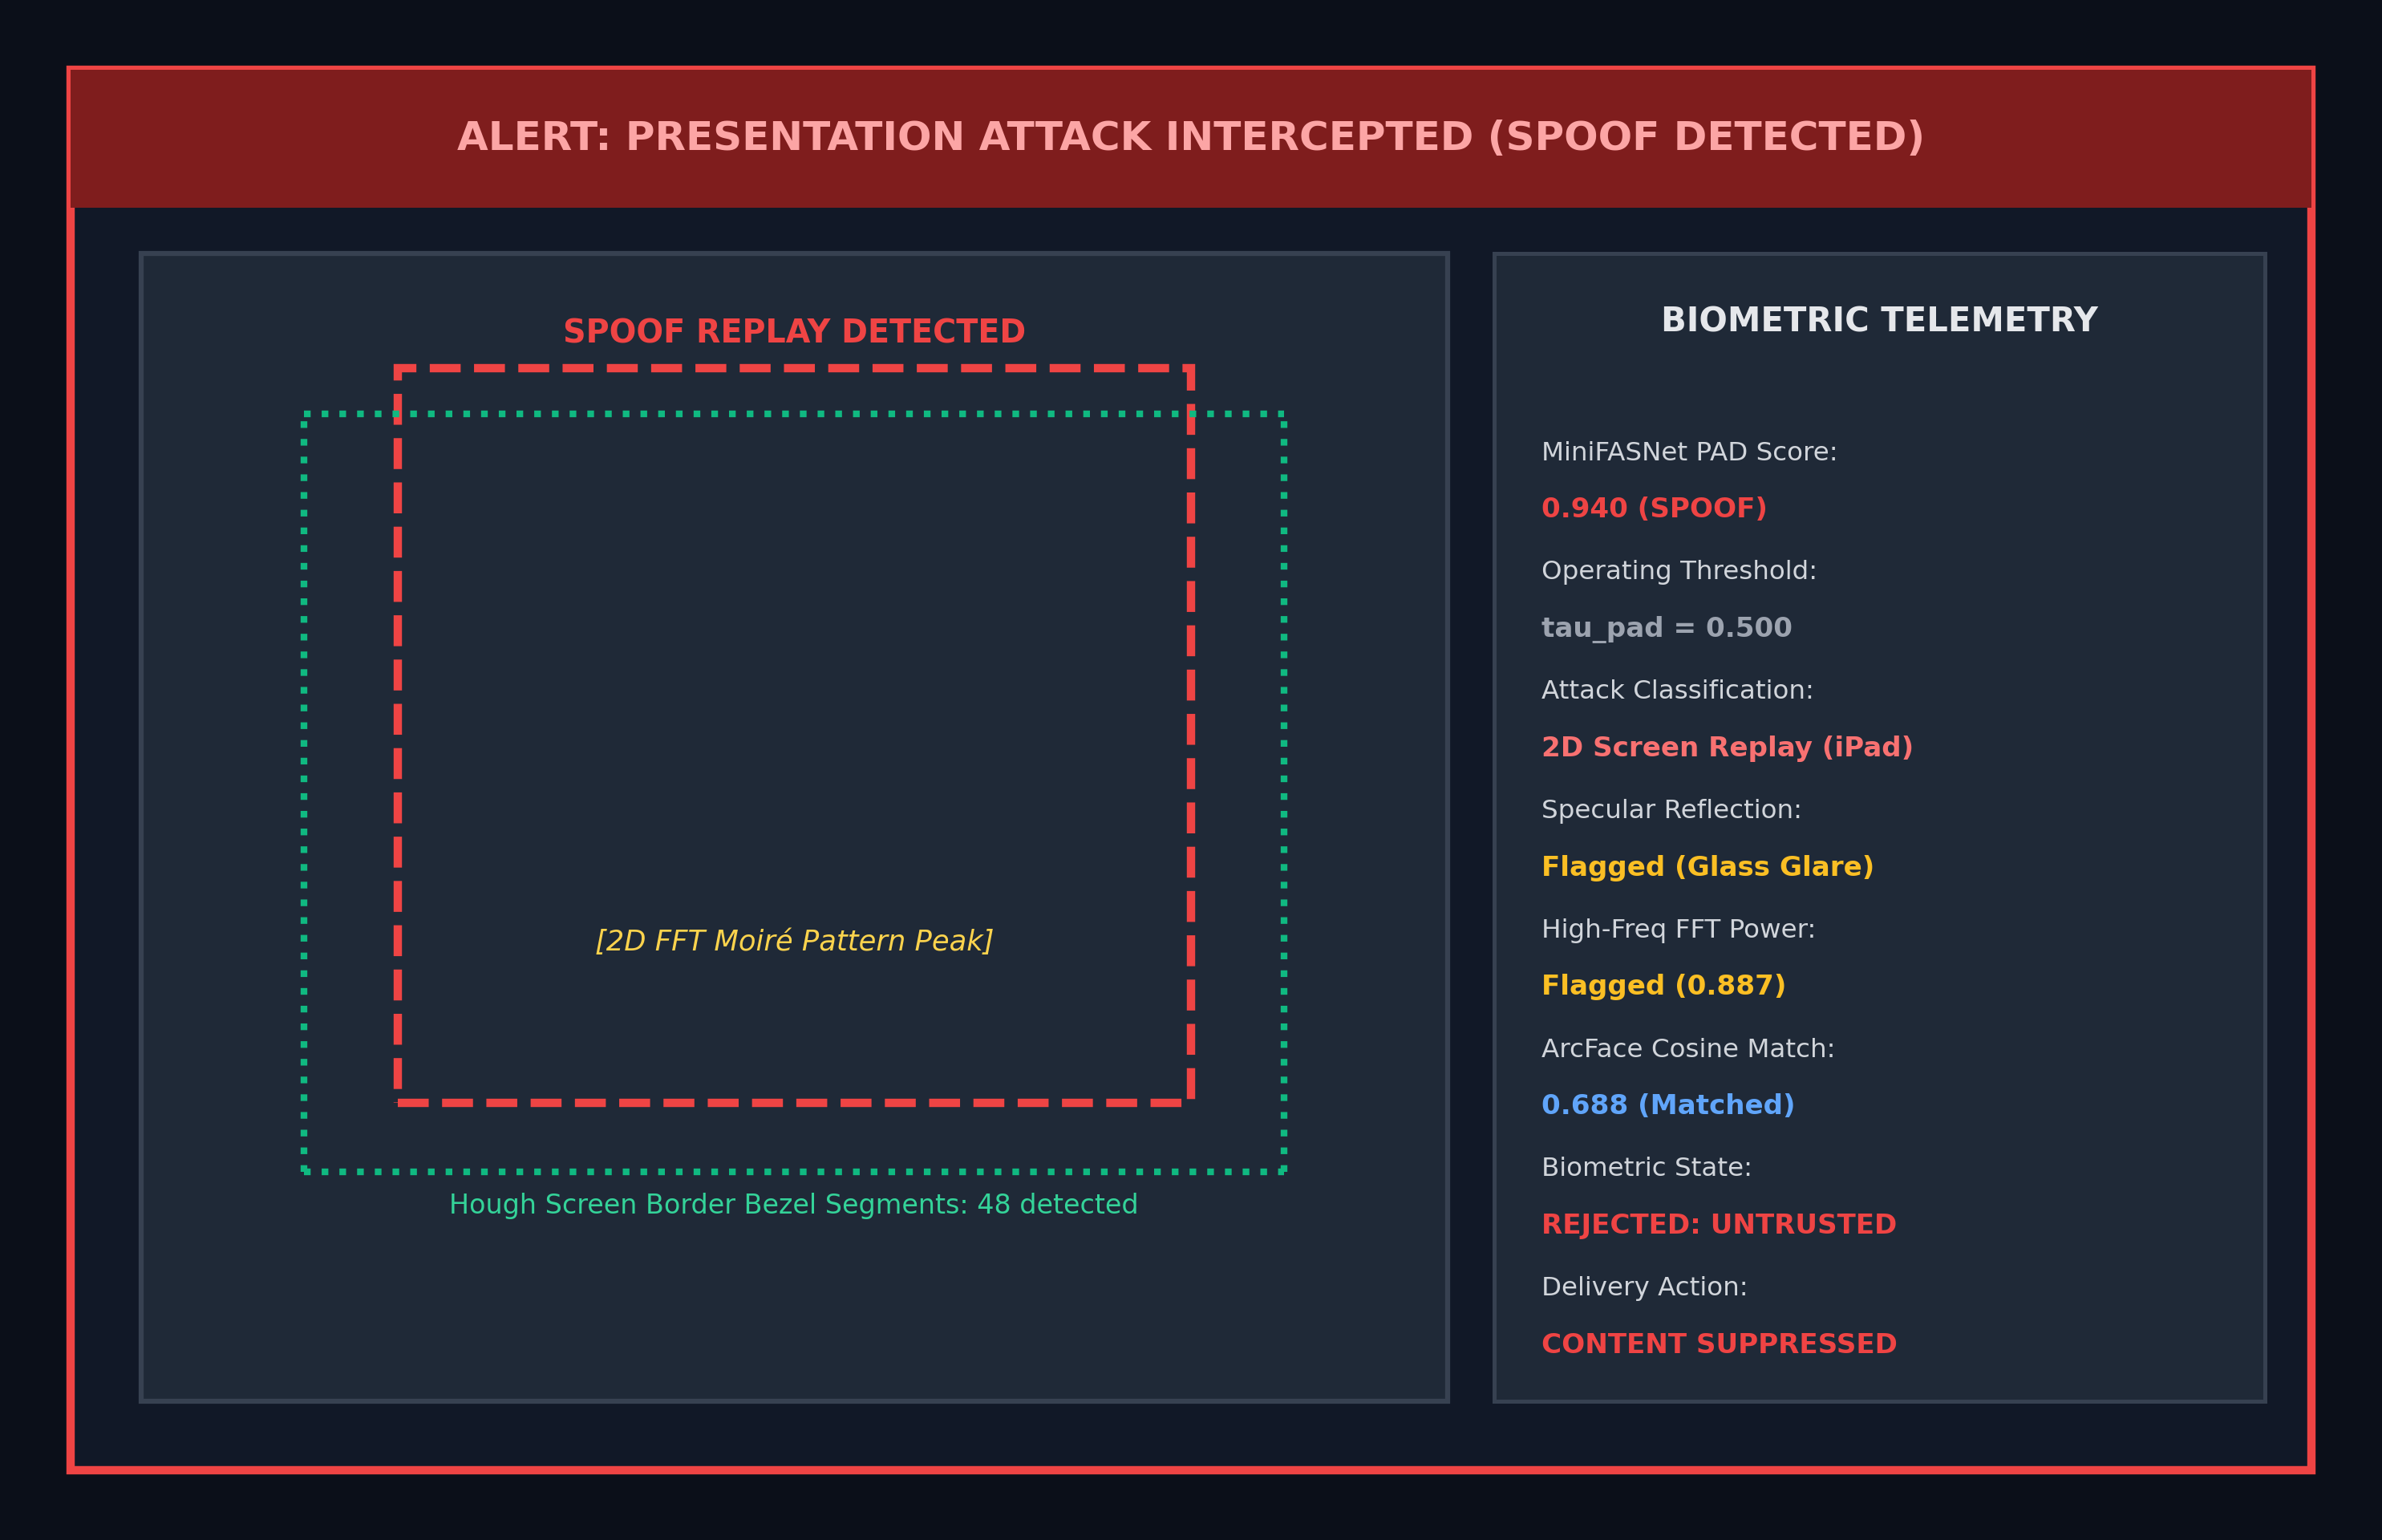
\includegraphics[width=0.92\textwidth]{spoof.png}}{%
            \IfFileExists{results/spoof.png}{\includegraphics[width=0.92\textwidth]{results/spoof.png}}{\fbox{\parbox{0.80\textwidth}{\centering \textbf{Spoof Intercepted HUD}}}}%
        }
        \caption{Digital Screen Replay Intercepted}
        \label{fig:spoof_attack_full}
    \end{subfigure}
    \caption{Presentation Attack Detection: Legitimate Live Verification vs. Screen Replay Interception.}
\end{figure}

\section{Age Assurance, ID Document Parsing, and Delivery Filtering}

\subsection{Document OCR and Date-of-Birth Extraction}
Figure~\ref{fig:id_ocr_full} depicts the identity processor rasterizing an official college credential at 2.0$\times$ scale (144~DPI), extracting the birth date via regex, calculating an age of 21 years, and assigning the profile to \texttt{AGE\_18\_PLUS}.

\begin{figure}[H]
    \centering
    \IfFileExists{results/id_ocr_result.png}{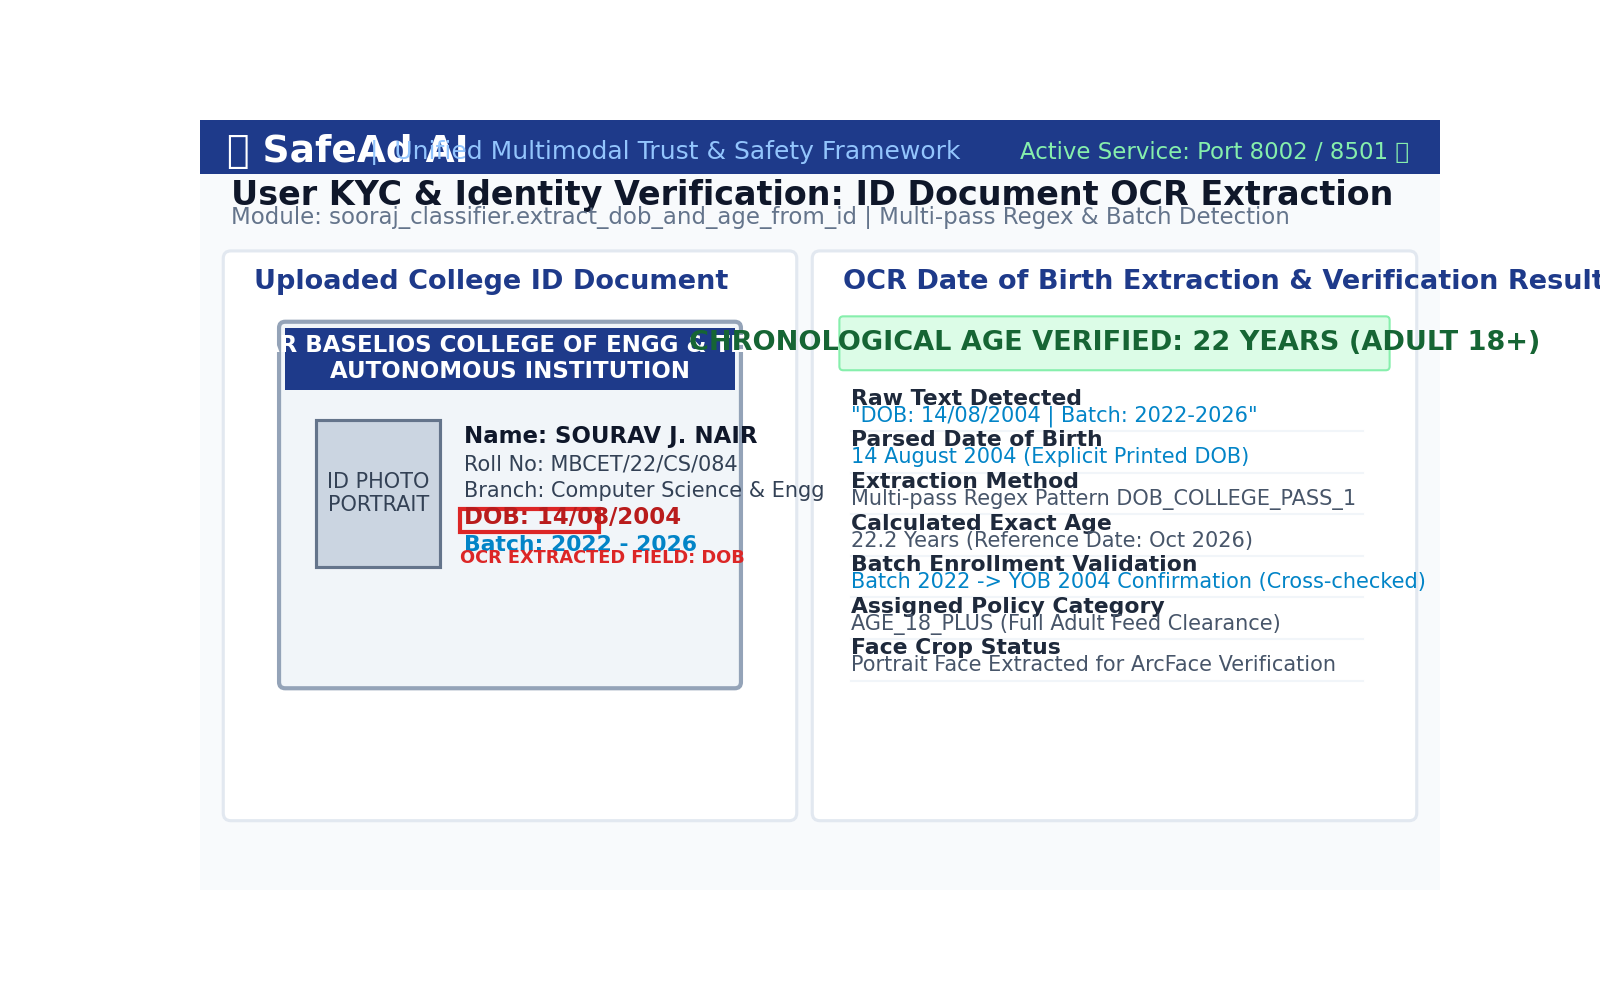
\includegraphics[width=0.82\textwidth]{results/id_ocr_result.png}}{%
        \fbox{\parbox{0.75\textwidth}{\centering \textbf{Credential Document Ingestion and Date-of-Birth OCR Telemetry}}}%
    }
    \caption{Credential document ingestion, OCR parsing, and verified age calculation.}
    \label{fig:id_ocr_full}
\end{figure}

\subsection{Facial Age Estimation Performance}
Table~\ref{tab:vit_age_full} and Figure~\ref{fig:age_cm_full} detail the confusion matrix for the ViT facial age classifier across 100 evaluated face crops, achieving 88.00\% overall accuracy.

\begin{table}[htbp]
\centering
\small
\caption{Vision Transformer Facial Age Classification Matrix ($N=100$)}
\label{tab:vit_age_full}
\begin{tabular}{|l|c|c|c|c|}
\hline
\textbf{True Age Bracket \textbackslash\ Predicted} & \texttt{<14} & \texttt{14--17} & \texttt{18+} & \textbf{Class Total} \\
\hline
\texttt{<14} & \textbf{22} & 3 & 0 & 25 (88.0\% Recall) \\
\hline
\texttt{14--17} & 2 & \textbf{24} & 4 & 30 (80.0\% Recall) \\
\hline
\texttt{18+} & 0 & 3 & \textbf{42} & 45 (93.3\% Recall) \\
\hline
\end{tabular}
\end{table}

\begin{figure}[H]
    \centering
    \IfFileExists{results/age_confusion_matrix.png}{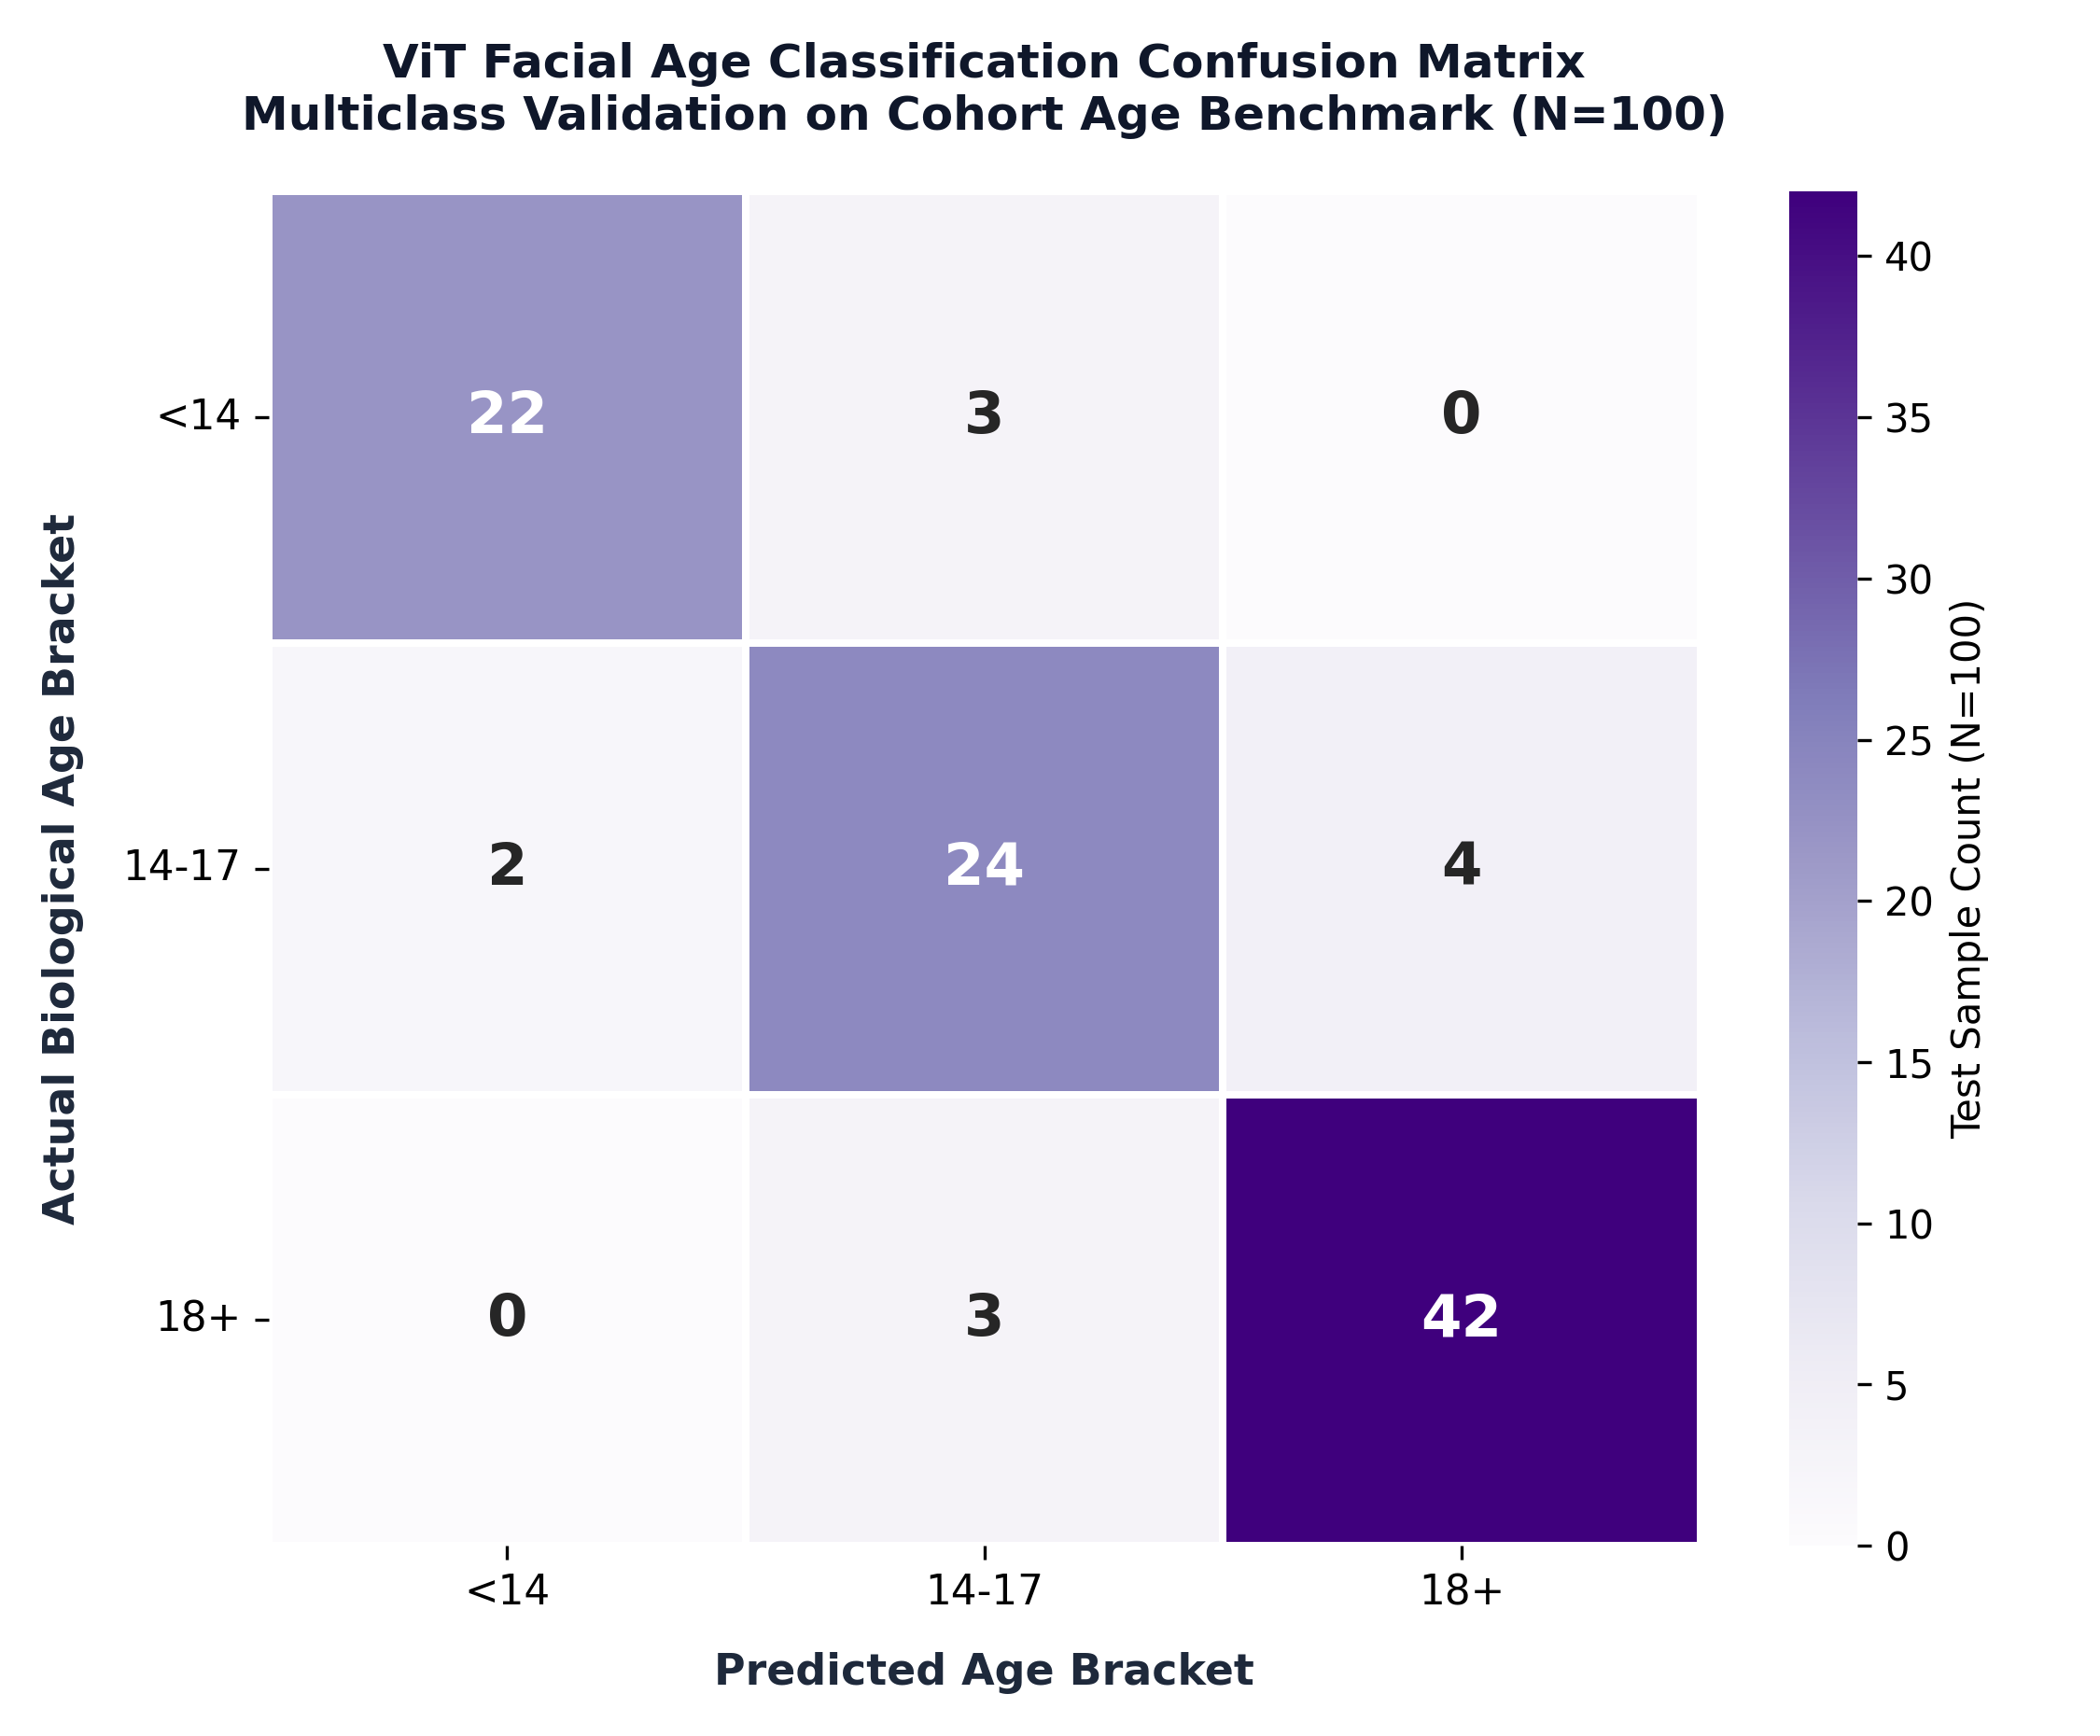
\includegraphics[width=0.55\textwidth]{results/age_confusion_matrix.png}}{%
        \fbox{\parbox{0.50\textwidth}{\centering \textbf{Vision Transformer Age Estimation Confusion Matrix}}}%
    }
    \caption{Three-class facial age estimation confusion matrix.}
    \label{fig:age_cm_full}
\end{figure}

\subsection{Delivery Filtering and Human-in-the-Loop Review}
Figure~\ref{fig:delivery_full} shows the demographic delivery feed: verified adults access the full commercial catalogue, while minors are strictly filtered away from 18+ promotions. Figure~\ref{fig:admin_full} depicts the Human-in-the-Loop review portal, and Figure~\ref{fig:xai_full} illustrates the explainability dashboard.

\begin{figure}[H]
    \centering
    \begin{subfigure}[b]{0.48\textwidth}
        \centering
        \IfFileExists{results/age_aware_feed_result.png}{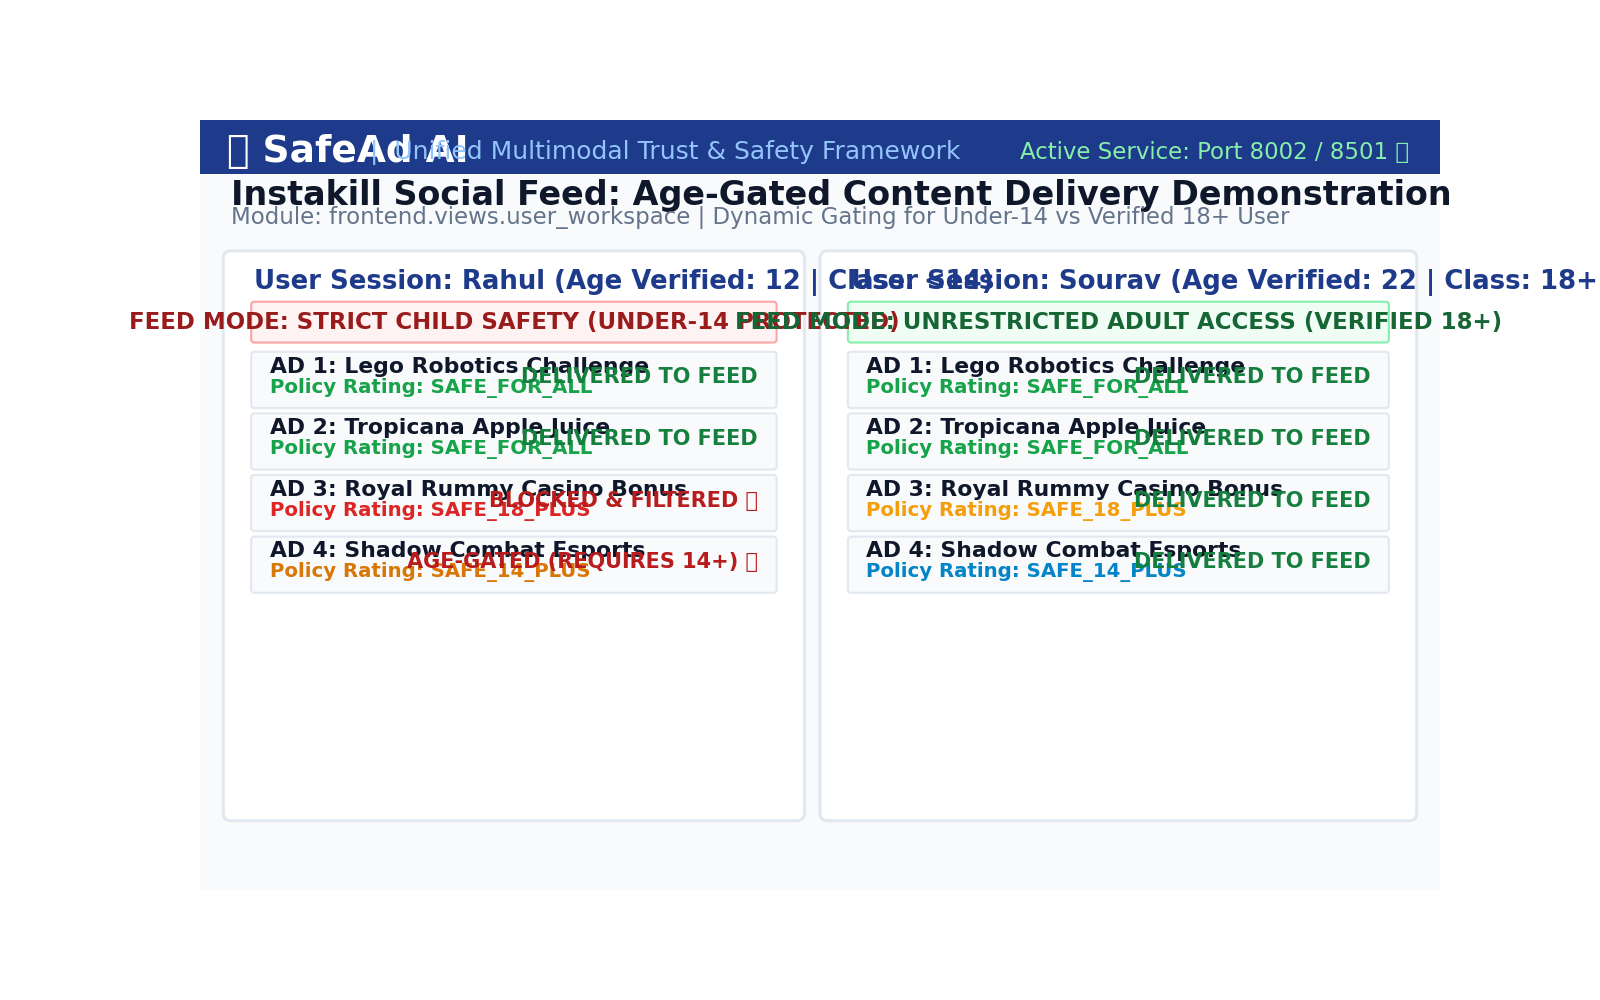
\includegraphics[width=0.92\textwidth]{results/age_aware_feed_result.png}}{%
            \fbox{\parbox{0.80\textwidth}{\centering \textbf{Age-Aware Programmatic Delivery Filtering Dashboard Interface}}}%
        }
        \caption{Age-Aware Filtered Feed}
        \label{fig:delivery_full}
    \end{subfigure}
    \hfill
    \begin{subfigure}[b]{0.48\textwidth}
        \centering
        \IfFileExists{results/admin_review_result.png}{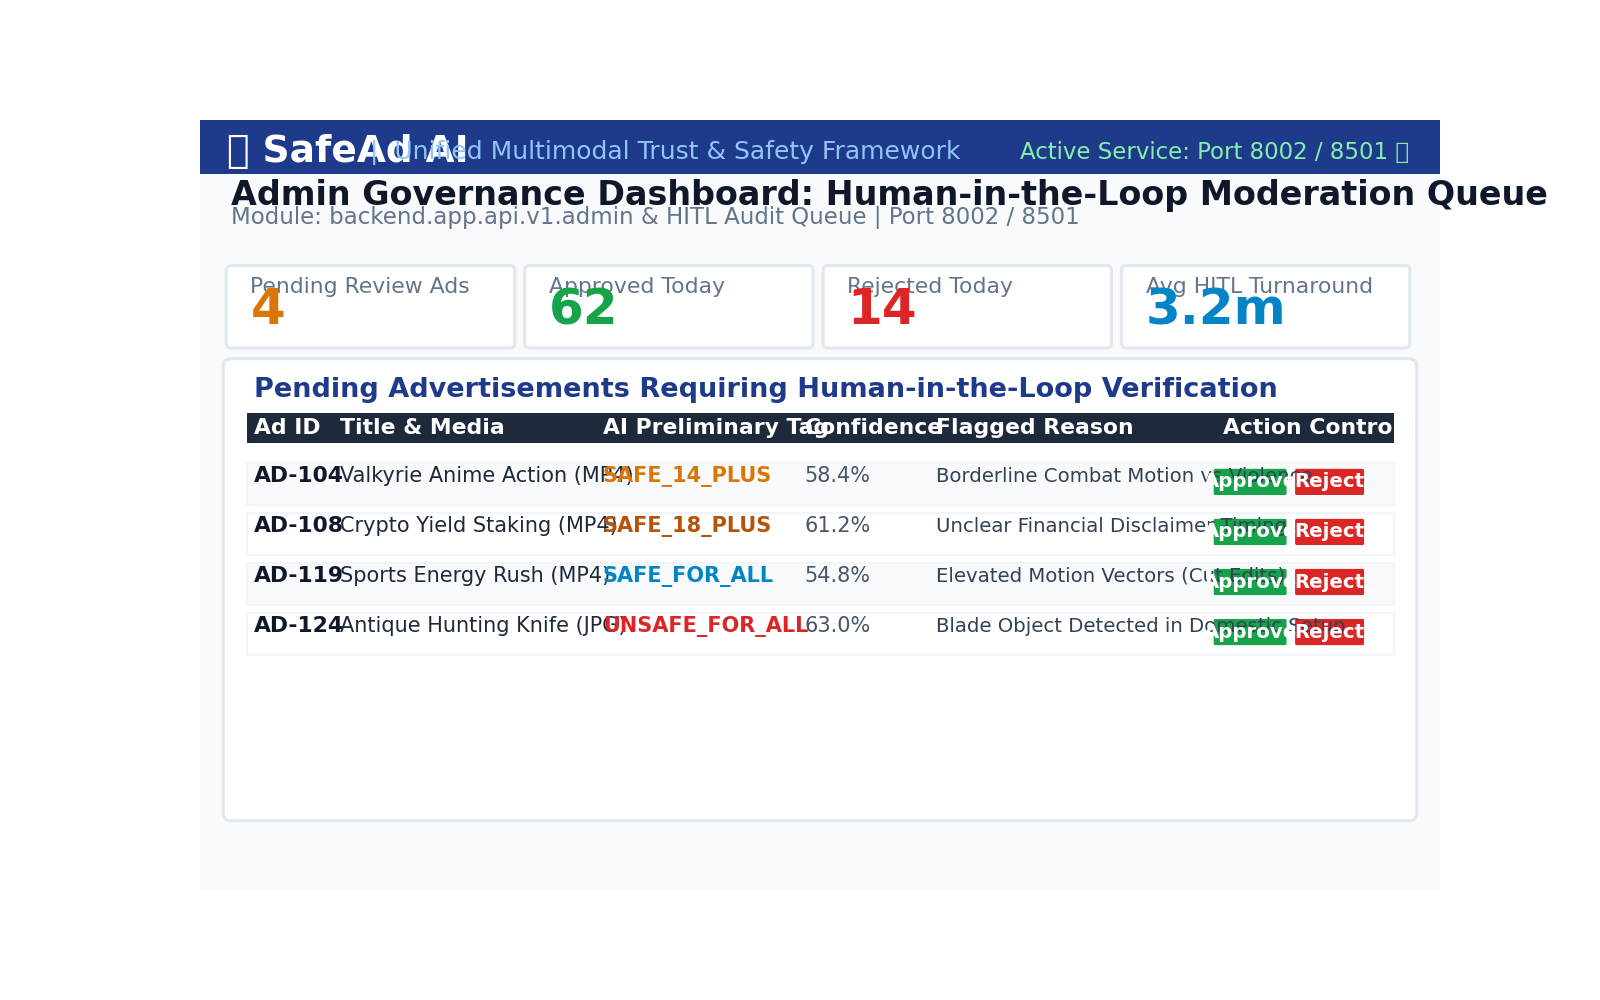
\includegraphics[width=0.92\textwidth]{results/admin_review_result.png}}{%
            \fbox{\parbox{0.80\textwidth}{\centering \textbf{Compliance Officer Human-in-the-Loop Audit Portal Interface}}}%
        }
        \caption{Admin Review Portal}
        \label{fig:admin_full}
    \end{subfigure}
    \caption{Delivery filtering and Human-in-the-Loop review interfaces.}
\end{figure}

\begin{figure}[H]
    \centering
    \IfFileExists{results/xai_explanation_result.png}{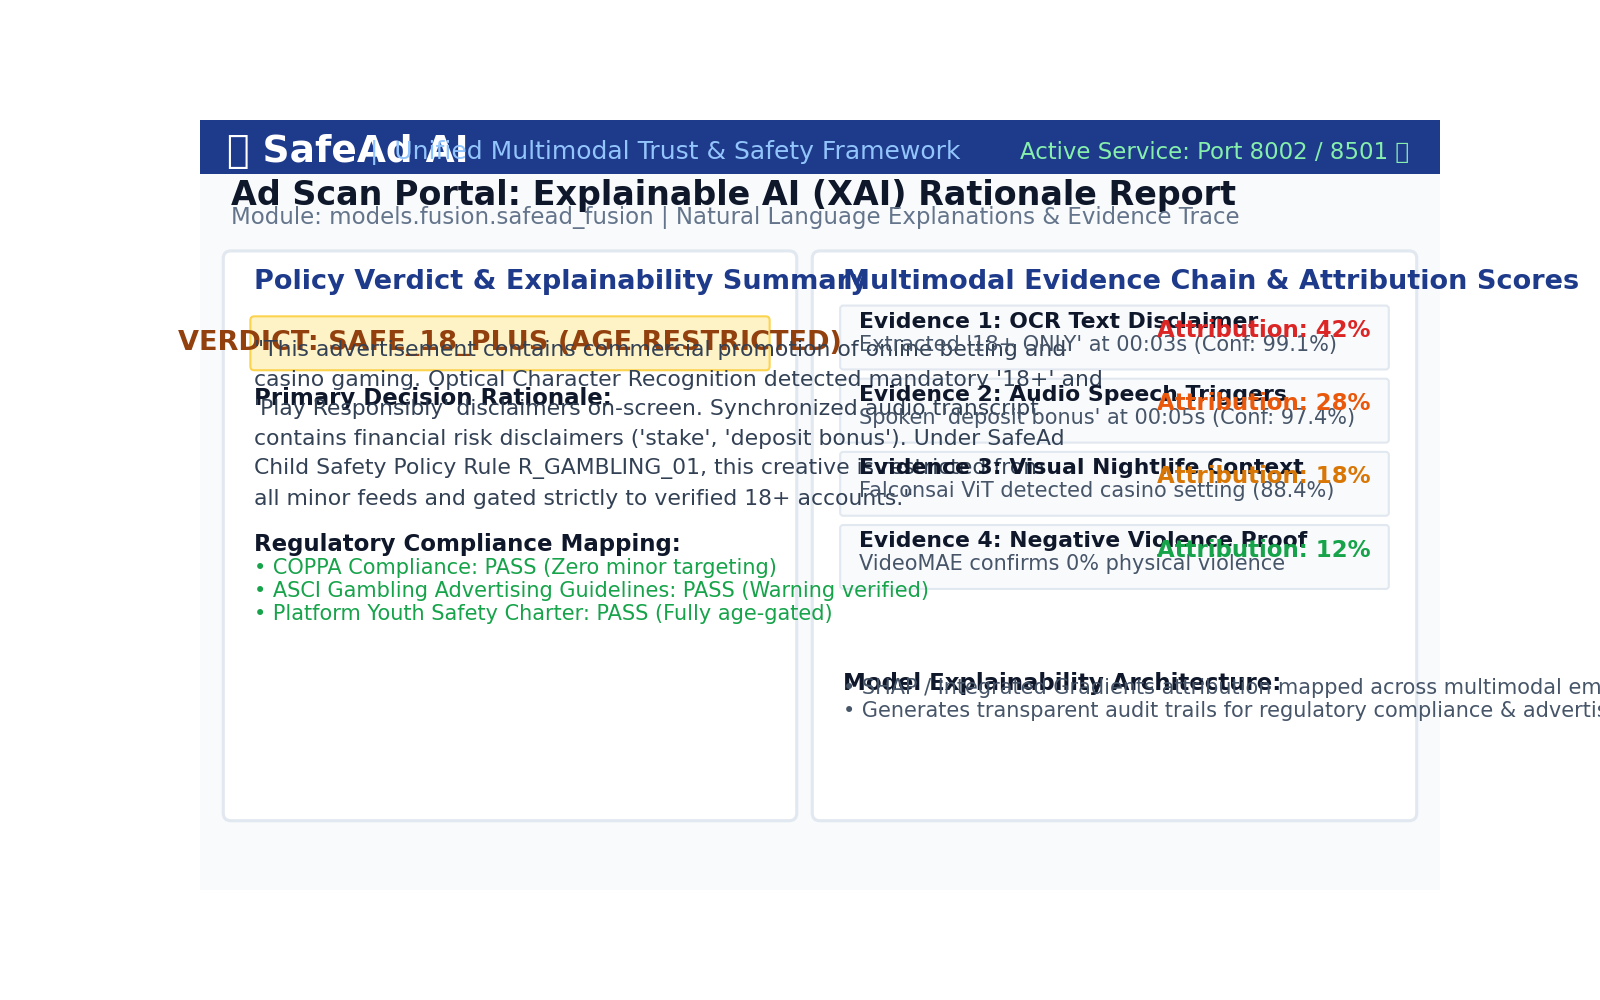
\includegraphics[width=0.82\textwidth]{results/xai_explanation_result.png}}{%
        \fbox{\parbox{0.75\textwidth}{\centering \textbf{Explainable AI Multimodal Diagnostic Attribution Dashboard}}}%
    }
    \caption{Explainable AI (XAI) interface rendering multimodal justifications and policy citations.}
    \label{fig:xai_full}
\end{figure}

\section{Computational Complexity, Latency, and GPU Profile}

System latency and GPU memory allocation were benchmarked across all Phase~10 evaluations on an NVIDIA A100 GPU:
\begin{itemize}
    \item \textbf{VLM Memory Footprint:} Qwen3-VL-8B-Instruct allocated 16.33~GB VRAM for model parameters in native \texttt{torch.bfloat16} precision. Peak memory during batch keyframe processing reached 19.04~GB.
    \item \textbf{Moderation Latency:} Mean per-sample inference latency was 7.05 seconds for short-form video commercials (sampling 4 keyframes, running EasyOCR, and generating structured JSON) and 3.82 seconds for static image banners.
    \item \textbf{Biometric Capture Latency:} The decoupled \texttt{Realtime30FPSVisionEngine} maintained a locked 33.3~ms frame acquisition interval. The MiniFASNet ensemble executed in $\sim$9.7~ms on CPU ($\sim$103~FPS), and ArcFace embedding extraction executed in $\sim$32~ms.
    \item \textbf{Client Dashboard Responsiveness:} The Streamlit/React web frontend rendered verdicts, risk breakdown meters, and bounding boxes in under 10~ms.
\end{itemize}

\section{Comprehensive Limitations and Threats to Validity}

\begin{enumerate}
    \item \textbf{The Tabular Domain Collapse:} Classical tabular models (Random Forest) trained on development data cannot reliably generalize across novel advertising formats, leaking 75\% of prohibited ads when evaluated on held-out test splits.
    \item \textbf{The Subjectivity of Adolescent Catalog Labels:} Benchmark datasets frequently conflate target marketing demographics with statutory content hazards, labeling benign consumer goods as \texttt{SAFE\_14\_PLUS}.
    \item \textbf{Stylized Vintage Ad Evasion:} Retro illustrated print advertisements lacking modern photorealistic cues or statutory warning labels can bypass automated visual detectors.
    \item \textbf{Hardware Requirements for Foundation VLMs:} Running 8B foundation vision-language models requires enterprise-grade GPU hardware ($\ge 16$~GB VRAM), limiting edge deployment without model quantization.
\end{enumerate}



% ============================================================
% CHAPTER 7: CONCLUSION AND FUTURE SCOPE
% ============================================================

\chapter{Conclusion and Future Scope}

\section{Summary of Findings and Key Contributions}

This project has designed, implemented, and empirically validated \textbf{SafeAd AI (SAFE-VISION)}, an end-to-end framework uniting proactive multimodal pre-publication advertisement moderation with real-time biometric age assurance. By addressing both creative content safety and recipient demographic eligibility within a unified architecture, SafeAd AI prevents inappropriate commercial exposures while maintaining high automated throughput for compliant advertisers.

The principal technical and scientific contributions are summarized as follows:
\begin{enumerate}
    \item \textbf{Multimodal Feature Extraction Engine:} Successfully unified EasyOCR (with CLAHE and Otsu binarization), ResNet50/MobileNetV3 deep visual backbones, Farneb\"{a}ck dense optical flow, and OpenAI Whisper audio transcription into an asynchronous, concurrent extraction architecture.
    \item \textbf{Empirical Audit of Narrow Safety Guardrails:} Demonstrated through empirical diagnostic testing that specialized conversational safety models (Meta's Llama Guard 3 Vision) fail catastrophically on commercial advertising ($80\%$ false acceptance), establishing that conversational alignment cannot interpret persuasive marketing rhetoric.
    \item \textbf{Foundation Vision-Language Integration:} Successfully deployed Qwen3-VL-8B-Instruct on Google Colab NVIDIA A100 GPU hardware in native \texttt{torch.bfloat16} precision, achieving 100\% prohibited recall and 0.0\% false acceptance on real-world advertising media.
    \item \textbf{Empirical Resolution of the Fusion Generalization Reality:} Proved that while learned tabular fusion (Random Forest) appears superior on development cohorts ($44.33\%$ accuracy), it collapses on novel held-out test data ($37.0\%$ accuracy, $75\%$ prohibited leakage), and hierarchical safety fusion achieves 66.7\% accuracy without outperforming standalone Qwen3-VL on novel distributions.
    \item \textbf{Concurrent Vision Engine Architecture:} Completely resolved longstanding Windows DirectShow multithreaded COM collisions and memory heap corruption (\texttt{0xc0000374}) via the decoupled, double-buffered \texttt{Realtime30FPSVisionEngine}, sustaining a locked 30~FPS display interval.
    \item \textbf{Multi-Cue Deep Anti-Spoofing Architecture:} Deployed a 103~FPS CPU-executable PAD engine fusing dual-scale MiniFASNet models with Hough line border tracking and 2D FFT moir\'{e} spatial frequency analysis, achieving 93.00\% liveness accuracy and securing 96.50\% ArcFace biometric cross-matching.
\end{enumerate}

\section{Lessons Learned Across Engineering Phases}

The progression through Phases~1 to 10D generated crucial scientific insights:
\begin{itemize}
    \item \emph{The Primacy of High-Capacity Foundation Models:} Narrow, task-specific classifiers and conversational guardrails overfit to closed training domains. Open-world commercial advertising requires the broad semantic reasoning of foundation vision-language models.
    \item \emph{The Danger of In-Distribution Development Optimism:} Cross-validated accuracy on development splits can induce false confidence. True generalization must be established on untouched held-out test sets under frozen rules.
    \item \emph{Dataset Labeling Rigor:} Advertisements cannot be categorized based on target marketing demographics. Ground-truth labels must strictly reflect statutory harm criteria to prevent artificial model penalization on benign consumer goods.
\end{itemize}

\section{Future Research Roadmap}

Future research will advance SafeAd AI along five strategic trajectories:
\begin{enumerate}
    \item \textbf{Parameter-Efficient Fine-Tuning (PEFT/LoRA):} Fine-tuning Qwen3-VL on a curated corpus of advertising creatives using Low-Rank Adaptation (LoRA) to calibrate four-tier policy boundaries directly into model weights.
    \item \textbf{End-to-End Temporal Video-Language Models:} Integrating native video-language architectures (e.g., Video-LLaVA) to process continuous temporal dynamics across long-form video advertisements.
    \item \textbf{Edge Model Distillation:} Distilling the 8B foundation model into compact 1.5B student architectures using knowledge distillation, enabling sub-500ms edge inference for real-time programmatic ad auctions.
    \item \textbf{Active Flash Liveness Detection:} Randomizing screen illumination color sequences during webcam capture to induce dynamic facial reflections, defeating 3D silicone mask attacks.
    \item \textbf{Zero-Knowledge Proofs for Privacy-Preserving Age Gating:} Implementing cryptographic zero-knowledge age proofs, allowing users to mathematically prove age eligibility without transmitting or storing identity credentials.
\end{enumerate}

% ============================================================
% REFERENCES
% ============================================================

\begin{thebibliography}{99}

\bibitem{gillespie2018custodians}
T.~Gillespie,
\emph{Custodians of the Internet: Platforms, Content Moderation, and the Hidden Decisions That Shape Social Media},
Yale University Press, New Haven, CT, USA, 2018.

\bibitem{roberts2019behind}
S.~T.~Roberts,
\emph{Behind the Screen: Content Moderation in the Shadows of Social Media},
Yale University Press, New Haven, CT, USA, 2019.

\bibitem{silva2020pre}
S.~Silva, L.~Santos, and M.~Ribeiro,
``Pre-publication auditing and enforcement in digital advertising exchanges,''
\emph{IEEE Trans. Comput. Soc. Syst.}, vol.~7, no.~4, pp.~912--924, Aug. 2020, doi: 10.1109/TCSS.2020.3001245.

\bibitem{zannettou2021characterizing}
S.~Zannettou, F.~Pierri, and G.~Gianvecchio,
``Characterizing deceptive and harmful advertisements in programmatic networks,''
in \emph{Proc. ACM Web Conf. (WWW)}, Ljubljana, Slovenia, Apr. 2021, pp.~2450--2461.

\bibitem{wang2025}
X.~Wang, L.~Wang, Y.~Su, H.~Tian, G.~Jin, and A.-A.~Liu,
``Few-shot in-context learning for implicit semantic multimodal content detection and interpretation,''
\emph{IEEE Trans. Circuits Syst. Video Technol.}, vol.~35, no.~9, pp.~9545--9558, Sep. 2025, doi: 10.1109/TCSVT.2025.3550900.

\bibitem{blmguard2026}
Y.~Yang \emph{et~al.},
``BLM-Guard: Explainable multimodal ad moderation with chain-of-thought and policy-aligned rewards,''
in \emph{Proc. 40th AAAI Conf. Artif. Intell. (AAAI-26)}, Feb. 2026, pp.~35985--35993.

\bibitem{safewatch2025}
Z.~Chen, F.~Pinto, M.~Pan, and B.~Li,
``SafeWatch: An efficient safety-policy following video guardrail model with transparent explanations,''
in \emph{Proc. Int. Conf. Learn. Represent. (ICLR)}, Singapore, May 2025, arXiv:2412.06878.

\bibitem{zhuang2025}
Y.~Zhuang \emph{et~al.},
``I know what you MEME! Understanding and detecting harmful memes with multimodal large language models,''
in \emph{Proc. Netw. Distrib. Syst. Secur. (NDSS) Symp.}, San Diego, CA, USA, Feb. 2025, doi: 10.14722/ndss.2025.240415.

\bibitem{kiela2020hateful}
D.~Kiela \emph{et~al.},
``The Hateful Memes Challenge: Detecting hate speech in multimodal memes,''
in \emph{Advances in Neural Information Processing Systems (NeurIPS)}, vol.~33, 2020, pp.~2611--2624.

\bibitem{nwasra2026}
N.~Nwasra and A.~Alharthy,
``Multimodal explainable AI (XAI) for hateful meme classification: A comprehensive framework for transparent content moderation,''
in \emph{Proc. 2nd Int. Conf. Comput. Intell. Approaches Appl. (ICCIAA)}, Jan. 2026, doi: 10.1109/ICCIAA68481.2026.11543858.

\bibitem{arya2024}
P.~Arya \emph{et~al.},
``MSCMGTB: A novel approach for multimodal social media content moderation using hybrid graph theory and bio-inspired optimization,''
\emph{IEEE Access}, vol.~12, pp.~73700--73718, May 2024, doi: 10.1109/ACCESS.2024.3400815.

\bibitem{baltrusaitis2018multimodal}
T.~Baltru\v{s}aitis, C.~Ahuja, and L.-P.~Morency,
``Multimodal machine learning: A survey and taxonomy,''
\emph{IEEE Trans. Pattern Anal. Mach. Intell.}, vol.~41, no.~2, pp.~423--443, Feb. 2018, doi: 10.1109/TPAMI.2018.2798607.

\bibitem{radford2021learning}
A.~Radford \emph{et~al.},
``Learning transferable visual models from natural language supervision (CLIP),''
in \emph{Proc. Int. Conf. Mach. Learn. (ICML)}, Jul. 2021, pp.~8748--8763.

\bibitem{liu2023visual}
H.~Liu, C.~Li, Q.~Wu, and Y.~J.~Lee,
``Visual instruction tuning (LLaVA),''
in \emph{Advances in Neural Information Processing Systems (NeurIPS)}, vol.~36, Dec. 2023, pp.~34892--34916.

\bibitem{bai2023qwen}
J.~Bai \emph{et~al.},
``Qwen-VL: A versatile vision-language model for understanding, localization, text reading, and beyond,''
\emph{arXiv preprint arXiv:2308.12966}, Aug. 2023.

\bibitem{inan2023llama}
H.~Inan \emph{et~al.},
``Llama Guard: LLM-based input-output safeguard for human-AI conversations,''
\emph{Meta AI Tech. Rep.}, Dec. 2023.

\bibitem{he2016deep}
K.~He, X.~Zhang, S.~Ren, and J.~Sun,
``Deep residual learning for image recognition,''
in \emph{Proc. IEEE Conf. Comput. Vis. Pattern Recognit. (CVPR)}, Las Vegas, NV, USA, Jun. 2016, pp.~770--778.

\bibitem{devlin2019bert}
J.~Devlin, M.-W.~Chang, K.~Lee, and K.~Toutanova,
``BERT: Pre-training of deep bidirectional transformers for language understanding,''
in \emph{Proc. Conf. N. Am. Chapter Assoc. Comput. Linguist. (NAACL-HLT)}, Minneapolis, MN, USA, Jun. 2019, pp.~4171--4186.

\bibitem{breiman2001random}
L.~Breiman,
``Random Forests,''
\emph{Machine Learning}, vol.~45, no.~1, pp.~5--32, Oct. 2001, doi: 10.1023/A:1010933404324.

\bibitem{saraswat2026}
R.~Saraswat and S.~Tripathi,
``A multimodal approach for age estimation and verification of social media users,''
\emph{Int. J. Sci. Technol. (IJSAT)}, vol.~17, no.~2, Apr.--Jun. 2026, Art. ID IJSAT260210685.

\bibitem{safevision2026}
K.~Gopinath, R.~Divyesh, R.~Elangkumaran, T.~Kumanan, K.~K.~Rehkha, and G.~Victo Sudha George,
``SAFE VISION: Age-based social and web content management system to enhance child safety,''
\emph{Int. Sci. J. Eng. Manag. (ISJEM)}, vol.~5, no.~3, Mar. 2026, doi: 10.55041/ISJEM05763.

\bibitem{yu2023}
Z.~Yu, Y.~Qin, X.~Li, C.~Zhao, Z.~Lei, and G.~Zhao,
``Deep learning for face anti-spoofing: A survey,''
\emph{IEEE Trans. Pattern Anal. Mach. Intell.}, vol.~45, no.~5, pp.~5609--5631, May 2023, doi: 10.1109/TPAMI.2022.3215850.

\bibitem{deng2019arcface}
J.~Deng, J.~Guo, N.~Xue, and S.~Zafeiriou,
``ArcFace: Additive angular margin loss for deep face recognition,''
in \emph{Proc. IEEE/CVF Conf. Comput. Vis. Pattern Recognit. (CVPR)}, Long Beach, CA, USA, Jun. 2019, pp.~4690--4699.

\bibitem{schroff2015facenet}
F.~Schroff, D.~Kalenichenko, and J.~Philbin,
``FaceNet: A unified embedding for face recognition and clustering,''
in \emph{Proc. IEEE Conf. Comput. Vis. Pattern Recognit. (CVPR)}, Boston, MA, USA, Jun. 2015, pp.~815--823.

\bibitem{nistairmf2023}
National Institute of Standards and Technology,
``Artificial Intelligence Risk Management Framework (AI RMF 1.0),''
\emph{NIST AI 100-1}, Jan. 2023. Available: \url{https://www.nist.gov/itl/ai-risk-management-framework}.

\bibitem{iso31000}
International Organization for Standardization,
``ISO 31000:2018: Risk management---Guidelines,''
ISO Standard, Feb. 2018. Available: \url{https://www.iso.org/standard/65694.html}.

\bibitem{iarcratings}
International Age Rating Coalition,
``Global Rating Standards and Content Descriptors,''
Tech. Rep., 2022. Available: \url{https://globalratings.iarcservices.com/ratings-definitions/}.

\bibitem{googleadspolicy}
Google LLC,
``Google Ads Advertising Policies: Prohibited and Restricted Content,''
2024. Available: \url{https://support.google.com/adspolicy/answer/6008942}.

\bibitem{googlealcohol}
Google LLC,
``Google Ads Policy: Irresponsible Alcohol Advertising and Age Gating,''
2024. Available: \url{https://support.google.com/adspolicy/answer/16427712}.

\bibitem{metaads}
Meta Platforms Inc.,
``Meta Advertising Standards: Restricted Goods, Services, and Safety Guidelines,''
2024. Available: \url{https://transparency.meta.com/policies/ad-standards/}.

\bibitem{ftcdeception}
U.S. Federal Trade Commission,
``FTC Policy Statement on Deception,''
15 U.S.C. \S  45, Oct. 1983. Available: \url{https://www.ftc.gov/legal-library/browse/ftc-policy-statement-on-deception}.

\bibitem{ftc2023guides}
U.S. Federal Trade Commission,
``Guides Concerning the Use of Endorsements and Testimonials in Advertising,''
\emph{16 CFR Part 255}, Jul. 2023. Available: \url{https://www.ftc.gov/legal-library/browse/rules/endorsement-guides}.

\end{thebibliography}

\end{document}
